% Settings
\ifEMBED
    \setcounter{tocdepth}{4}   %= Aufnahme in das Inhaltsverzeichnis *
    \setcounter{secnumdepth}{4}  % = Nummerierung vertiefen *
\fi

% title page
\ifSTANDALONE
    \ifDC
        \begin{titlepage}

\begin{center}

% Oberer Teil der Titelseite:
%\includegraphics[width=0.15\textwidth]{./logo}\\[1cm]    
\textsc{\LARGE Produktentwicklung 2}\\[1.5cm]

\textsc{\Large Hochschule Luzern\\
    ~\\
    Technik \& Architektur}\\[0.5cm]

\vfill{}

% Title
\newcommand{\HRule}{\rule{\linewidth}{0.5mm}}
\HRule \\[0.4cm]
{   \Huge \bfseries DC Treiber\\
        ~\\
        \large Konzeptbeschreibung}\\[0.4cm]

\HRule \\[1.5cm]

% Author and supervisor
\begin{minipage}[t]{0.4\textwidth}
    \begin{flushleft} \large
        \emph{Autoren:}\\
        Ervin \textsc{Mazlagi\'c}\\
        Flavio \textsc{Kreiliger}\\
    \end{flushleft}
\end{minipage}
\hfill
\begin{minipage}[t]{0.4\textwidth}
    \begin{flushright} \large
        \emph{Projektgruppe:} \\
        PREN-ET
    \end{flushright}
\end{minipage}

\vfill{}
\vfill{}
\vfill{}

% Unterer Teil der Seite
{\large Horw\\ \today}

\end{center}

\end{titlepage}

    \fi
    \ifBLDC
        \begin{titlepage}

\begin{center}

% Oberer Teil der Titelseite:
%\includegraphics[width=0.15\textwidth]{./logo}\\[1cm]    
\textsc{\LARGE Produktentwicklung 1}\\[1.5cm]

\textsc{\Large Hochschule Luzern\\
    ~\\
    Technik \& Architektur}\\[0.5cm]

\vfill{}

% Title
\newcommand{\HRule}{\rule{\linewidth}{0.5mm}}
\HRule \\[0.4cm]
{   \Huge \bfseries Brushless DC Treiber\\
        ~\\
        \large Konzeptbeschreibung}\\[0.4cm]

\HRule \\[1.5cm]

% Author and supervisor
\begin{minipage}{0.4\textwidth}
    \begin{flushleft} \large
        \emph{Autoren:}\\
        Yves \textsc{Studer}\\
        Daniel \textsc{Winz}\\
        Ervin \textsc{Mazlagi\'c}\\
    \end{flushleft}
\end{minipage}
\hfill
\begin{minipage}{0.4\textwidth}
    \begin{flushright} \large
        \emph{Projektgruppe:} \\
        PREN-ET
    \end{flushright}
\end{minipage}

\vfill{}
\vfill{}
\vfill{}

% Unterer Teil der Seite
{\large Horw\\ \today}

\end{center}

\end{titlepage}

    \fi
    \ifSTEPPER
        \begin{titlepage}

\begin{center}

% Oberer Teil der Titelseite:
%\includegraphics[width=0.15\textwidth]{./logo}\\[1cm]    
\textsc{\LARGE Produktentwicklung 1}\\[1.5cm]

\textsc{\Large Hochschule Luzern\\
    ~\\
    Technik \& Architektur}\\[0.5cm]

\vfill{}

% Title
\newcommand{\HRule}{\rule{\linewidth}{0.5mm}}
\HRule \\[0.4cm]
{   \Huge \bfseries Stepper Treiber\\
        ~\\
        \large Konzeptbeschreibung}\\[0.4cm]

\HRule \\[1.5cm]

% Author and supervisor
\begin{minipage}{0.4\textwidth}
    \begin{flushleft} \large
        \emph{Autorin:}\\
        Bettina \textsc{Wyss}\\
    \end{flushleft}
\end{minipage}
\hfill
\begin{minipage}{0.4\textwidth}
    \begin{flushright} \large
        \emph{Projektgruppe:} \\
        PREN-ET
    \end{flushright}
\end{minipage}

\vfill{}
\vfill{}
\vfill{}

% Unterer Teil der Seite
{\large Horw\\ \today}

\end{center}

\end{titlepage}

    \fi    
    \ifREVIEW
        \begin{titlepage}

\begin{center}

% Oberer Teil der Titelseite:
%\includegraphics[width=0.15\textwidth]{./logo}\\[1cm]    
\textsc{\LARGE Produktentwicklung 2}\\[1.5cm]

\textsc{\Large Hochschule Luzern\\
    ~\\
    Technik \& Architektur}\\[0.5cm]

\vfill{}

% Title
\newcommand{\HRule}{\rule{\linewidth}{0.5mm}}
\HRule \\[0.4cm]
{   \Huge \bfseries Review ET-Gruppe\\
        ~\\
        \large Rückblick auf die ET-Zusammenarbeit}\\[0.4cm]

\HRule \\[1.5cm]

% Author and supervisor
\begin{minipage}[t]{0.4\textwidth}
    \begin{flushleft} \large
        \emph{Autoren:}\\
        Ervin \textsc{Mazlagi\'c}\\
        Flavio \textsc{Kreiliger}\\
        Bettina \textsc{Wyss}\\
        Daniel \textsc{Winz}\\
        Yves \textsc{Studer}\\
    \end{flushleft}
\end{minipage}
\hfill
\begin{minipage}[t]{0.4\textwidth}
    \begin{flushright} \large
        \emph{Projektgruppe:} \\
        PREN-ET
    \end{flushright}
\end{minipage}

\vfill{}
\vfill{}
\vfill{}

% Unterer Teil der Seite
{\large Horw\\ \today}

\end{center}

\end{titlepage}

    \fi
\else
    \author{PREN-ET}
    \maketitle
\fi

% Content
\tableofcontents
\clearpage
\ifSTANDALONE
\section{Fachgruppe Elektrotechnik}
\fi
\ifEMBED
\subsection{Fachgruppe Elektrotechnik}
\label{chap:Fachgruppe Elektrotechnik}
\fi
Elektrotechnik-Studierende aus mehreren Gruppen schliessen sich
zusammen, um gemeinsame Probleme anzugehen. Dabei handelt es sich
um die benötigte Hard- und Software, um Motoren anzusteuern
und gegebenenfalls zu regeln. In diesem Zusammenschluss werden drei Gruppen
gebildet, um Lösungen für DC-, Stepper- und Brushless-Motoren auszuarbeiten.
Die Idee besteht darin, dass nicht jede Gruppe für dasselbe Problem womöglich 
denselben Lösungsansatz verfolgt, sondern die Ressourcen kombiniert,
Synergien nutzt, um eine bessere Lösung zu erarbeiten. Auf diese Weise kann
das teamübergreifende Arbeiten im Rahmen des PREN erlernt und
geübt werden. Somit wird die Idee der Interdisziplinarität im erweiterten Sinn
Rechnung getragen. Die Gruppen und deren Mitglieder sind in 
\autoref{tab:pren-et-members} aufgeführt.
\begin{table}[h!]
    \centering
    \begin{zebratabular}{lllccc}
        \rowcolor{gray} 
        Team & Mitglied         & Github-Name & DC          & BLDC        & Stepper     \\
        27   & Daniel Winz      & daniw       &             & \textbullet & \textbullet \\
        32   & Yves Studer      & ystuder     &             & \textbullet &             \\
        33   & Flavio Kreiliger & Flavinsky   & \textbullet &             & \textbullet \\
        38   & Bettina Wyss     & BettyET     &             &             & \textbullet \\
        39   & Ervin Mazlagi\'c & ninux       & \textbullet &             &             \\
    \end{zebratabular}
    \caption{Übersicht der PREN-ET Projektgruppen}
    \label{tab:pren-et-members}
\end{table}

\noindent
Für den Austausch und die Ablage von Daten und Unterlagen wird die Plattform 
Github ausgewählt, da damit via Git\footnote{Verteiltes 
Versionskontrollsystem} versioniert werden kann. Dazu wird auf Github die 
Organisation PREN-ET gegründet. Diese ist unter 
\url{https://github.com/PREN-ET} einsehbar. für die einzelnen Projekte werden 
Repositorys angelegt. Diese sind in \autoref{tab:pren-et-repos} aufgeführt. 
\begin{table}[h!]
    \centering
    \begin{zebratabular}{p{0.09\textwidth}p{0.37\textwidth}p{0.4\textwidth}}
        \rowcolor{gray} 
        Repository  & Link         & Beschreibung \\
        info        & \url{https://github.com/PREN-ET/info}    & Allgemeine Informationen zur Organisation von PREN-ET \\
        doc         & \url{https://github.com/PREN-ET/doc}     & Dokumentation \\
        dc          & \url{https://github.com/PREN-ET/dc}      & Treiber für Gleichstrommotoren \\
        bldc        & \url{https://github.com/PREN-ET/bldc}    & Treiber für Brushless Motoren \\
        stepper     & \url{https://github.com/PREN-ET/stepper} & Treiber für Schrittmotoren \\
        frdm        & \url{https://github.com/PREN-ET/frdm}    & Beispiele zur Ansteuerung mittels FRDM-KL25Z \\
    \end{zebratabular}
    \caption{Übersicht der PREN-ET Repositorys}
    \label{tab:pren-et-repos}
\end{table}

\ifDC
    \renewcommand{\EtPath}{src/dc}
    \ifSTANDALONE
\section{Konzept}
\fi
\ifEMBED
\subsection{Konzept}
\fi

Das Stellen eines fremderregten Gleichstrommotors erfolgt über die
angelegte Ankerspannung. Eine variable Ankerspannung kann mittels einer 
zeitlichen Mittelung der anliegenden Spannung realisert werden. Somit
ist es möglich eine fremderregte Gleichstrommaschine mittels einer
konstanten Gleichspannung einzustellen. Die Mittelung der Ankerspannung
bildet die Basis des vorliegenden Konzepts für den DC-Motor Treiber.

\ifSTANDALONE
\subsection{Annahmen und Abschätzungen}\label{sec:annahmen}
\fi
\ifEMBED
\subsubsection{Annahmen und Abschätzungen}\label{sec:annahmen}
\fi
Für das vorliegende Konzept gilt die Annahme, dass das Erregerfeld mittels
Permanentmagneten realisiert ist und das Erregerfeld konstant ist. Diese
Annahme ist gewählt, da fremderregte Gleichstrommaschinen ohne
Permanentmagneten einen Erregerstrom benötigen, welcher das Erregerfeld
erzeugt. Im einfachsten Fall ist dies eine Kosntantstromquelle. Eine solche
Maschine benötigt mehr elektrische Energie und erfordert zusätzlichen
Hardwareaufwand.

Die Drehzahl einer idealen fremderregten Gleichstrommaschine mit konstantem
Erregerfeld korreliert mit $-1$ zum Strom. Der Strom einer solchen Maschine
korreliert widerum mit der Belastung \cite[p.163]{smps}. Dieses Verahalten
zwischen Belastung und Drehzahl ist in Abbildung \ref{fig:ideal-dc-curve}
dargestellt.

\begin{figure}[h!]
    \centering
    \begin{tikzpicture}
        % Achsen
        \draw[->] (-0.5,0) -- (8,0) node[anchor=north] {$I, M$};
        \draw[->] (0,-0.5) -- (0,4) node[anchor=east] {$\omega_m$};
        % Klemmenspannung
        \draw[blue, thick] (0,3) -- (7,3) node[anchor=west] {$U_K$};
        % induzierte Spannung
        \draw[red, thick] 
            (0,3) node[anchor=east] {$\omega_0$} -- 
            (7,0) node[midway, above right] {$\omega \sim U_i$};
        
    \end{tikzpicture}
    \caption{Winkelgeschwindigkeit einer idealen fremderregten 
        Gleichstrommaschine}
    \label{fig:ideal-dc-curve}
\end{figure}

\ifSTANDALONE
\subsection{Ziel}
\fi
\ifEMBED
\subsubsection{Ziel}
\fi
Es ist eine Hardware zu entwicklen, welche es ermöglicht, die
Winkelgeschwindigkeit einer fremerregten Gleichstrommaschine mit
Permanentmagneten zu regeln.

\ifSTANDALONE
\subsection{Funktionsweise}
\fi
\ifEMBED
\subsubsection{Funktionsweise}
\fi
Um die Klemmenspannung der Gleichstrommaschine zu stellen, wird eine
H-Brücke verwendet. Diese kann je nach Bedarf individuell ausgelegt
werden. Die Ansteuerung der H-Brücke erfolgt mittels des Treiberschips
A3941 von Allegro Microsystems. Das Interfaces, welches der
Treiberchip zur Verfügung stellt, wird mittels eines Mikrocontrollers
bedient, welcher ebenfalls individuell gewählt ist.

\begin{figure}[h!]
    \centering
    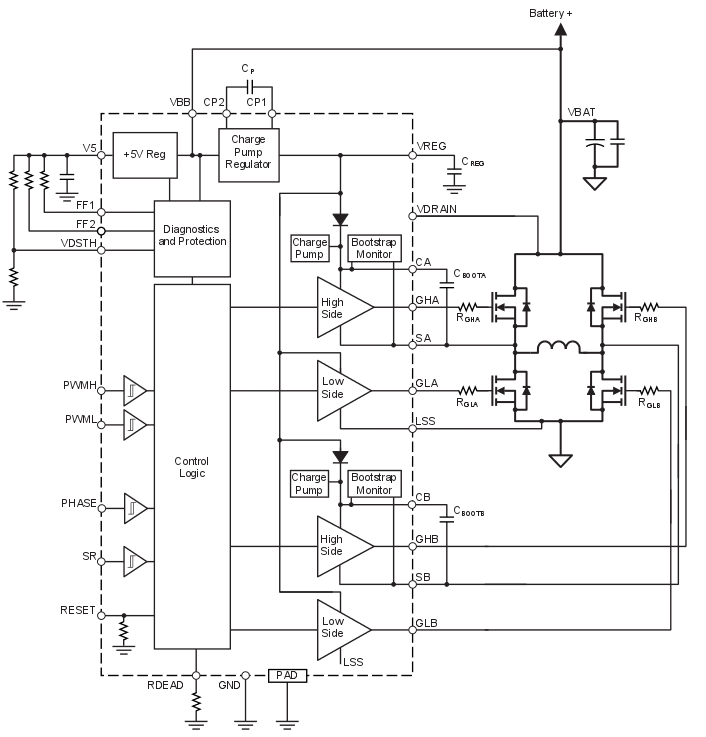
\includegraphics[width=0.75\textwidth]{\DCPath/fig/a3941-functional.png}
    \caption[Blockschaltbild des A3941]{Blockschaltbild des A3941 \cite{Datasheet:A3941}}
    \label{fig:a3941-functional}
\end{figure}

Die Regelung der Winkelgeschwindigkeit eines angeschlossenen Motors kann
mit verschiedenen Ansätzen realisert werden. Gemeinsam ist dabei stets die
Stellgrösse, welche durch das PWM Signal gegeben ist, als auch die
Winkelgeschwindigkeit der Maschine, welche die Regelgrösse darstellt.

Die Regelung muss auf einem Feedback der Winkelgeschwindigkeit basieren.
Wird von einer idealen Maschine ausgegangen, muss dieses Feedback nicht
zwingend durch einen Encoder generiert werden, sondern kann implizit durch
den Strom gegeben sein, wie in der Abbildung \ref{fig:ideal-dc-curve}
dargestellt. Mit den getroffenen Annahmen aus dem Abschnitt
\ref{sec:annahmen} kann somit auf ein explizites Feedback der
Winkelgeschwindigkeit verzichtet werden. 

\ifSTANDALONE
\subsection{Regelung}
\fi
\ifEMBED
\subsubsection{Regelung}
\fi
Für die Ansteuerung der H-Brücke bzw. des Treiberchips A3941 wird ein PWM
Signal benötigt. Dieses kann in Hardware auf dem Treiberboard implementiert
werden mittels eines Sägezahngenerators und einem Komparator. Der zweite
Komparatoreingang wird dazu an das Feedback des Stromes angeschlossen, was
ein zur Winkelgeschwindigkeit angepasstes PWM Signal generiert.

Alternativ zu dieser Regelung kann das Feedback des Stromes auch zum
Mikrocontroller geführt werden, welcher dieses auswertet und ein passendes
PWM Signal generiert.

\begin{figure}[h!]
    \centering
    \begin{subfigure}[b]{0.45\textwidth}
        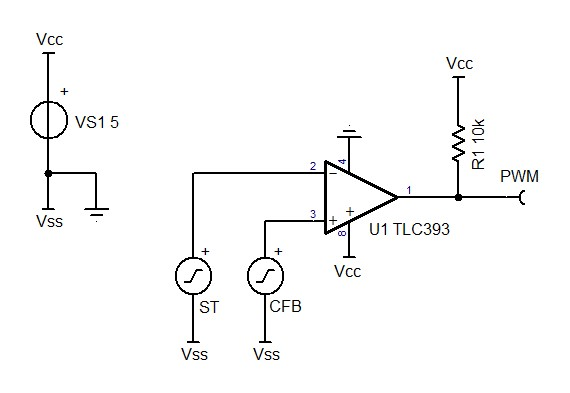
\includegraphics[width=\textwidth]{\DCPath/sim/sch-pwm-01.jpg}
        \caption{Prinzipschema mit dem Komparator TLC393}
    \end{subfigure}
    \begin{subfigure}[b]{0.45\textwidth}
        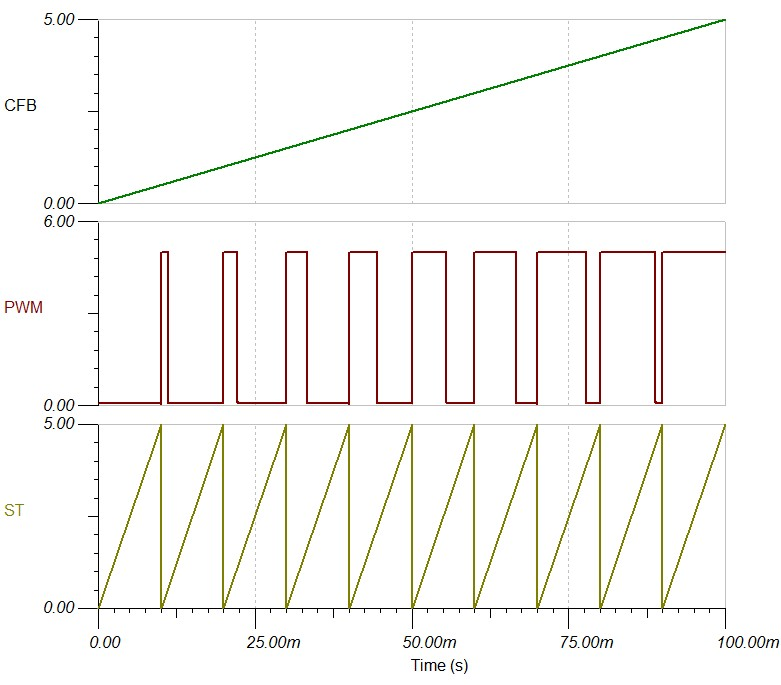
\includegraphics[width=\textwidth]{\DCPath/sim/pwm-01.jpg}
        \caption{Simulationsergebnisse für lineares Feedback}
    \end{subfigure}
    \caption{Simulation eines PWM-Generator mit Komparator}
\end{figure}

\begin{figure}[h!]
    \centering
    \begin{subfigure}[b]{0.45\textwidth}
        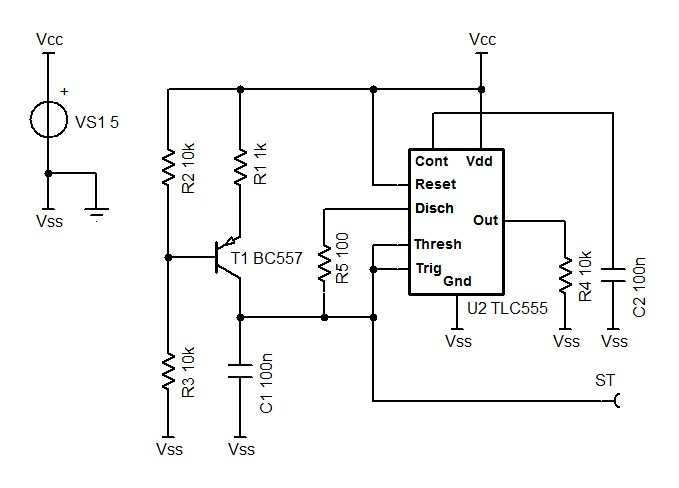
\includegraphics[width=\textwidth]{\DCPath/sim/sch-sawtooth-01.jpg}
        \caption{Sägezahntgenerator mit Timer TLC555}
    \end{subfigure}
    \begin{subfigure}[b]{0.45\textwidth}
        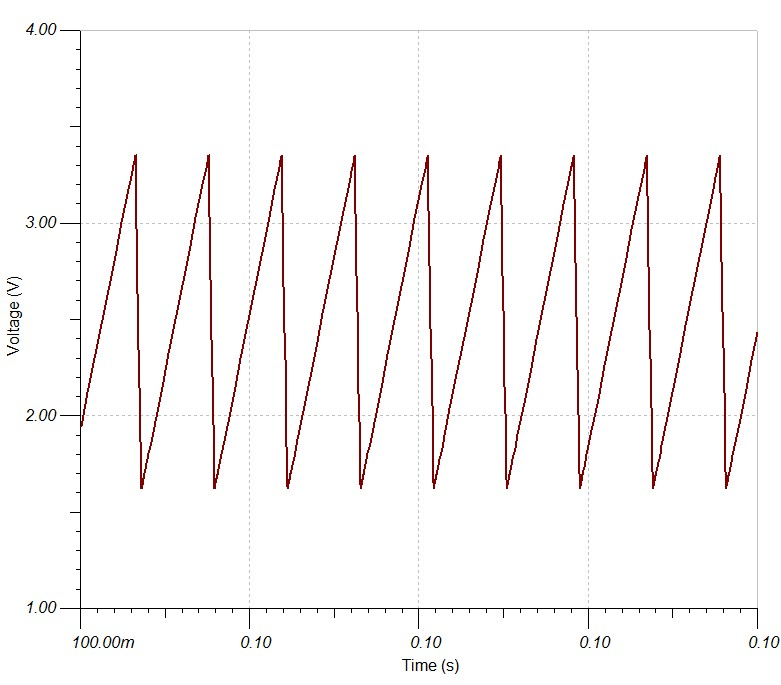
\includegraphics[width=\textwidth]{\DCPath/sim/sawtooth-01.jpg}
        \caption{Simulationsergebnisse ($f_{ST} \approx 9.3$kHz)}
    \end{subfigure}
    \caption{Simulation eines Sägezahngenerators}
    \label{fig:sawtooth}
\end{figure}

Ein passender Baustein zur Erzeugung ist der Timer TLC555, wie in der
Abbildung \ref{fig:sawtooth} dargestellt. Das Feedback des Stromes kann
dabei auf verschiedene Weise implementiert werden. Einerseits gibt es eine
kostengünstige Variante mittels dem Einsatz eines Shunt-Widerstands. Dieser
bietet im Idealfall ein lineares Varhalten. In der Realität führt der
Einfluss der Temperatur zu einer deutlichen nichtlinearität dieses
Messmittels. Eine Alternative zum Shunt-Widerstands bietet der Einsatz von
Hall-Effekt-Stromwandlern, welche den Strom linearisiert als Spannungssignal
ausgeben. Ein solcher Baustein ist der ACS712 der Allegro Microsystems,
welcher im SMD Format verfügbar ist bis zu einem Strom von 30A.

Ist eine genaue Drehzahl nicht von Bedeutung kann auf die Regelung der
Winkelgeschwindigkeit verzichtet werden. Dies gilt insbesondere, wenn eine
hohe Übersetzung vorliegt, welche verhindert, dass die Winkelgeschwindigkeit
der Gleichstrommaschine einbricht bei entsprechender Belastung. Für diesen
Fall kann das PWM fix eingestellt werden und lediglich mit einem Enable
Signal gearbeitet werden. Dies lässt sich mit einer logischen AND Funktion
realisieren für das PWM Signal. Eine mögliche Implementation ist in der
Abbildung \ref{fig:and} dargestellt.

\begin{figure}[h!]
    \centering
    \begin{subfigure}[b]{0.45\textwidth}
        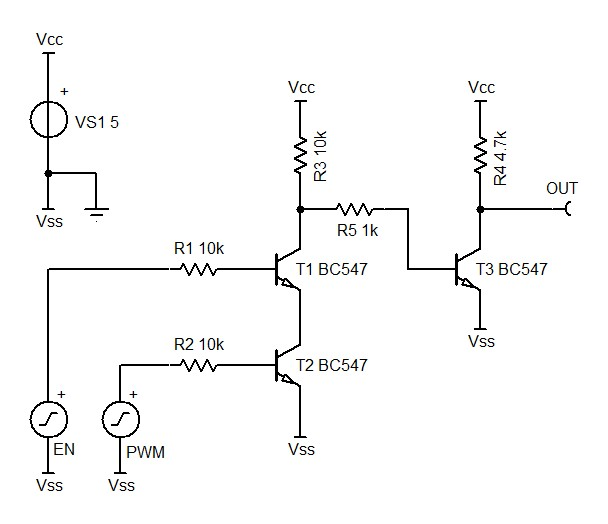
\includegraphics[width=\textwidth]{\DCPath/sim/sch-and-01.jpg}
        \caption{AND-Schaltung mit NPN-Transistoren}
    \end{subfigure}
    \begin{subfigure}[b]{0.45\textwidth}
        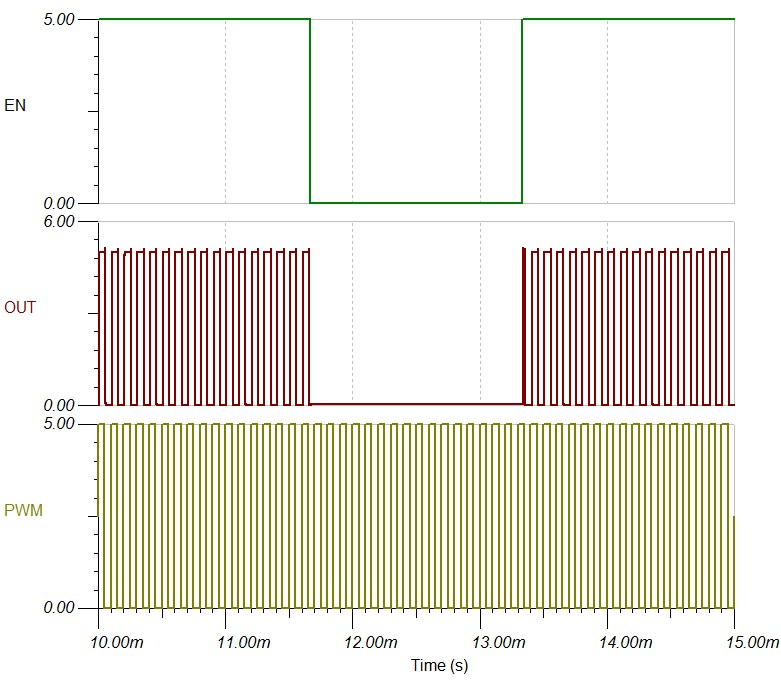
\includegraphics[width=\textwidth]{\DCPath/sim/and-01.jpg}
        \caption{Simulationsergebnisse}
    \end{subfigure}
    \caption{Simulation einer AND-Schaltung realisiert mit
        Bipolartransistoren}
    \label{fig:and}
\end{figure}


    \newpage
\section{Implementierung}

\subsection{Treiber}
Als Treiber für die H-Brücke wird der A3941 von Allegro verwendet. Dieser
Chip ist auf Farnell für ca. 8 CHF verfügbar und bietet eine einfache
DC-Motorenansteuerung mittels PWM-Signal und Richtungsangabe.

\subsubsection*{Eckdaten zum A3941 Treiberchip}
\begin{itemize}
	\item Spannung: 5.5 – 50V
	\item Geschwindigkeitseinstellung mittels PWM
	\item Richtungsbestimmung
	\item Preis: ca. 8 SFR
	\item Externe H-Brücke
\end{itemize}

\subsection{Timer}
Dieser Teil der Schaltung erzeugt das interne PWM-Signal. Mithilfe des
NE555 wird ein Sägezahnsignal erzeugt, welches auf den Komparator in IC1
geführt wird. Dieser Vergleicht diesen Sägezahn mit dem Schwellwert,
welcher mit dem Potentiometer R7 oder den beiden Widerständen R22 und R23
eingestellt werden kann (R22 und R23 sind eine Bestückungsvariante). 
Sobald er Sägezahn über dem Schwellwert ist, gibt der Komparator 15V aus.
Wenn der Sägezahn tiefer ist zieht er seinen Ausgang auf Ground. Da er
einen Open-Drain Ausgang hat, benötigt er einen Pull-UP Widerstand am
Ausgang.

\begin{figure}[h!]
	\centering
	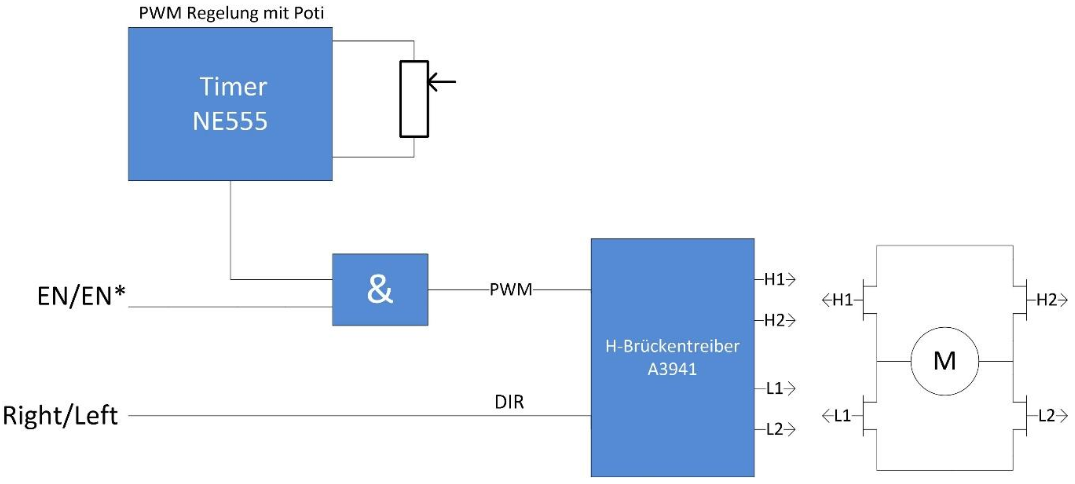
\includegraphics[width=0.75\textwidth]{src/dc/fig/timer_block.png}
	\caption{Blockschaltbild der Timerschaltung}
\end{figure}

\begin{figure}[h!]
	\centering
	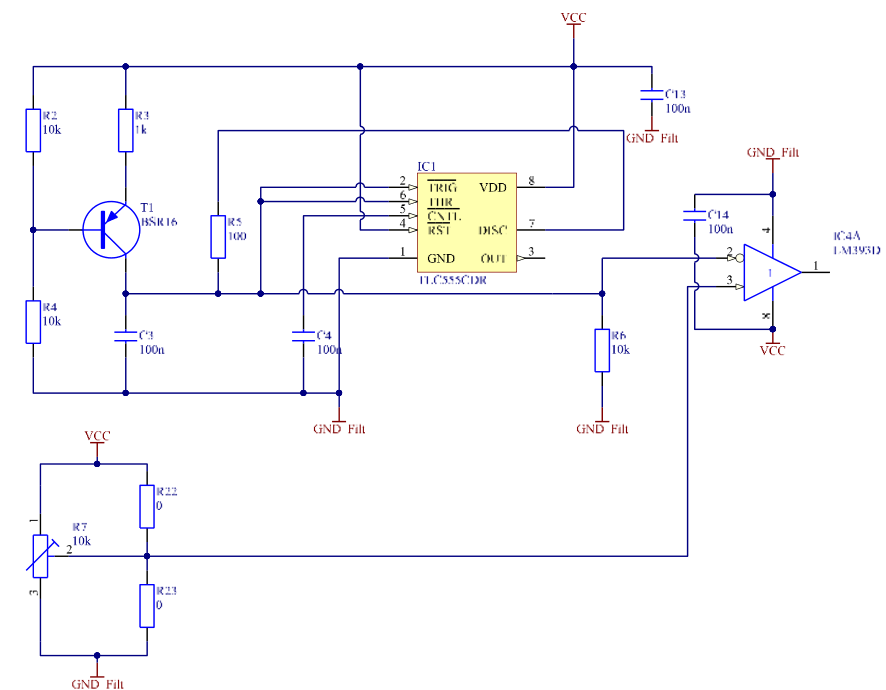
\includegraphics[width=0.75\textwidth]{src/dc/fig/timer_schematic.png}
	\caption{Timerschaltung}
\end{figure}

\newpage
\subsection{PWM-Logik}
Mit dieser Logik kann eingestellt werden, ob das interne oder ein externes
PWM Signal verwendet werden kann. Wird auf das Switch-Signal eine Logische
0 gelegt, wird das interne PWM verwendet, bei einer Logischen 1 das externe
PWM. Das Switch Signal kann auch als ON/OFF Signal für das interne PWM
verwendet werden. Dazu muss nur das externe PWM Signal dauerhaft auf Ground
geschaltet werden. Auf diese Art kann zwischen internem PWM und keinem PWM
umgeschaltet werden. Diese Betriebsart wird im Moment verwendet.

Die Zehnerdiode am Ausgang wird benötigt, um das Ausgangssignal auf den
Logikpegel des A3941 zu senken. Die 400x IC Reihe kann mit bis zu 18V
betrieben werden und gibt auch annähernd diese Spannung wieder aus. Da der
A3941 maximal einen Logikpegel von 6.5V verträgt, muss die Spannung
gesenkt werden.

\begin{figure}[h!]
	\centering
	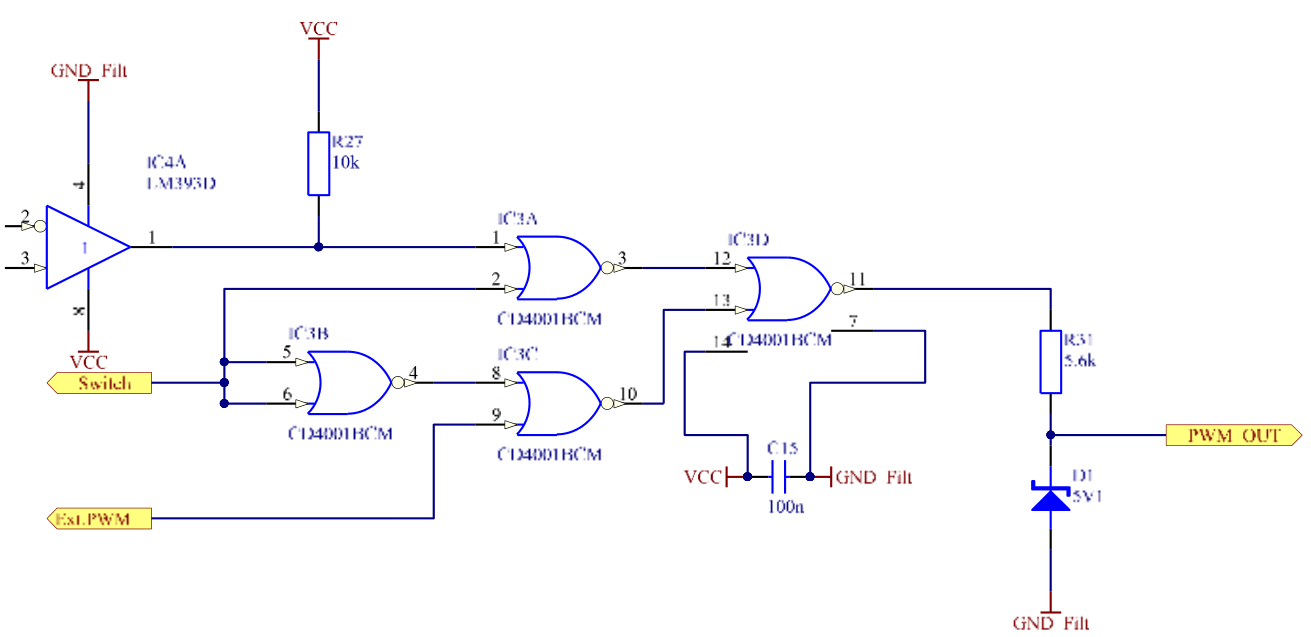
\includegraphics[width=0.75\textwidth]{src/dc/fig/pwm_schematic.png}
	\caption{PWM-Logik}
\end{figure}

\subsection{Ansteuerung}

\begin{figure}[h!]
	\centering
	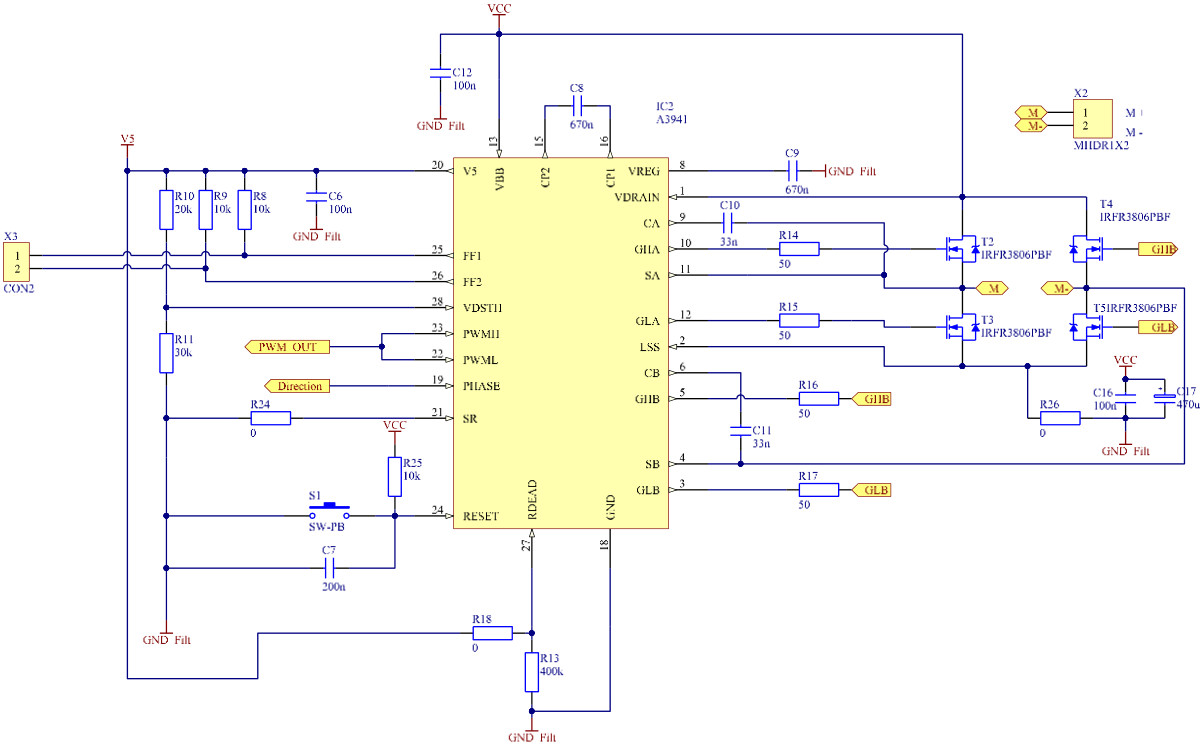
\includegraphics[width=0.75\textwidth]{src/dc/fig/driver_schematic.png}
	\caption{Treiberschaltung}
\end{figure}

Mit dem Phase-Eingang kann die Richtung eingestellt werden. Bei PWMH und
PWML wird das PWM Signal angeschlossen. Der Motorentreiber wird im
Fast-Decay Modus betrieben. Das heisst, die Spule des Motor wird beim
Abbremsen über die Dioden der H-Brücke entladen.

\begin{figure}[h!]
	\centering
	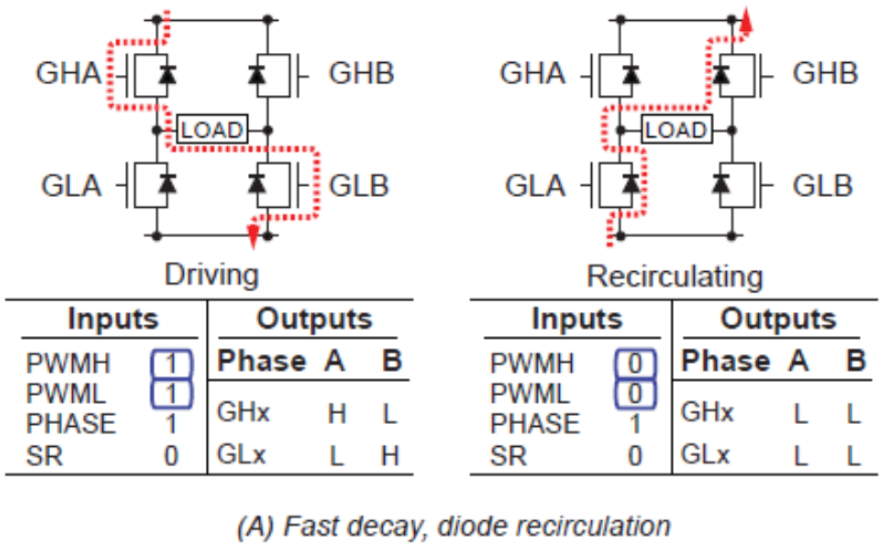
\includegraphics[width=0.5\textwidth]{src/dc/fig/decay.png}
	\caption{Fast Decay Illustation}
\end{figure}

\subsubsection{Ladungspumpe}
Die Ladungspumpe (Charge-Pump) wurde anhand des Datenblattes des A3941
und der eingesetzten MOSFET berechnet und eingesetzt. Die dazu notwendige
Kapazität ist wie folgt berechnet.

\[  
	C_{BOOT}
		= \frac{20 \cdot Q_{GATE}}{V_{BOOT}}
		= \frac{20 \cdot 30\mathrm{nC}}{10\mathrm{V}}
		= 33.3\mathrm{nF} 
		\xrightarrow{E6} 33\mathrm{nF}
\]

\noindent
Die Stützkapazität ist mit dem 20-fachen Wert zu belegen, also mit
\[
	C_{REG}
		\approx 20 \cdot C_{BOOT}
		= 20 \cdot 33\mathrm{nF}
		= 660\mathrm{nF}
\]

    \clearpage
\fi

\ifBLDC
    \renewcommand{\EtPath}{src/bldc}
    \ifSTANDALONE
\section{Brushless Motoransteuerung}
\fi
\ifEMBED
\subsubsection{Brushless Motoransteuerung}
\fi

\ifEMBED
    % Dieses Kapitel ist eine Zusammenarbeit der Gruppen \BLDCTeams. 
    \BLDCcollab
\fi
\ifSTANDALONE
    \subsection{Theorie der Ansteuerung}
    \fi
\ifEMBED
    \paragraph{Theorie der Ansteuerung}$~~$\\
    \fi
    \ifEMBED
        \begin{wrapfigure}{r}{0.50\textwidth}
           	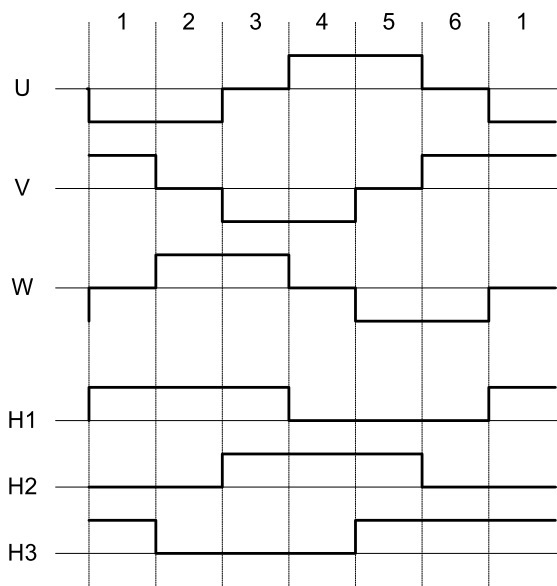
\includegraphics[scale=0.45]{\BLDCPath/Bilder/ZeitlicheHallSensorAnsteuerung.jpg}
         	\centering
           	\caption[Zeitliche Darstellung der Ansteuerung mit Hall-Sensoren]
           	{Zeitliche Darstellung der Ansteuerung mit Hall-Sensoren \cite{AppNote:BrushlessuC}}
            \label{abb:ZeitlicheAnsteuerungBrushlessMotor}
        \end{wrapfigure}
    \fi
        Brushless-Motoren (BLDC-Motoren) sind Synchron-Drehstrom-Motoren. Das 
        bedeutet, sie werden mittels eines kontinuierlichen magnetischen 
        Drehfeldes in Bewegung gesetzt.  Dabei ist darauf zu achten, dass der 
        Läufer dem Drehfeld synchron folgen kann, daher auch die 
        Namensbezeichnung des Motors. Falls der Läufer dem Drehfeld nicht 
        folgen kann, wird keine Spannung vom Rotor in die Statorwicklung 
        induziert, die der Erregerspannung entgegenwirkt. Daraus folgt, dass 
        ein immenser Strom fliesst, der nur von der Wicklungsimpedanz des 
        Motors begrenzt wird. Das Drehmoment ist abhängig vom Polradwinkel und 
        erreicht sein Maximum bei einem Polradwinkel von 90$^\circ$. Die 
        Kommutierung wird entweder als Sinuskommutierung oder als 
        Blockkommutierung ausgeführt. Die Sinuskommutierung bildet die 
        Sinusform eines dreiphasigen Netzes nach. Die Sinusform kann mit einem 
        Rechtecksignal angenähert werden. Dabei spricht man von einer 
        Blockkommutierung. Diese ist einfacher zu realisieren, aber erreicht 
        nicht das selbe Drehmoment wie eine Sinuskommutierung. In diesem 
        Projekt wird aufgrund der einfacheren Implementierung eine 
        Blockkommutierung realisiert. \\
    \ifSTANDALONE
        \begin{figure}[h!]
            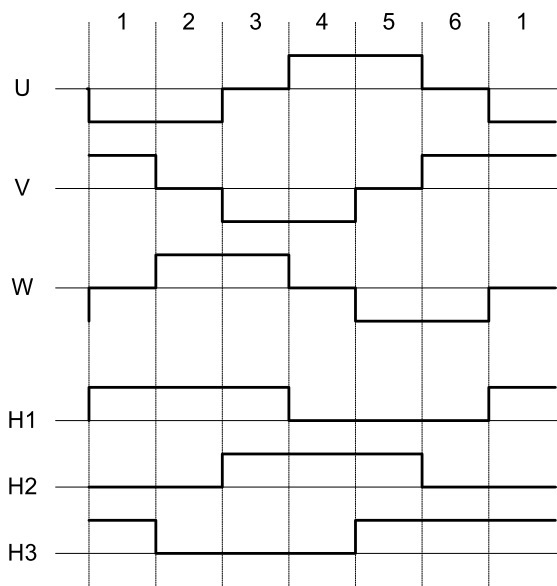
\includegraphics[scale=0.45]{\BLDCPath/Bilder/ZeitlicheHallSensorAnsteuerung.jpg}
            \centering
            \caption[Zeitliche Darstellung der Ansteuerung mit Hall-Sensoren]
            {Zeitliche Darstellung der Ansteuerung mit Hall-Sensoren \cite{AppNote:BrushlessuC}}
            \label{abb:ZeitlicheAnsteuerungBrushlessMotor}
        \end{figure}
    \fi
        \\
        Es gibt hauptsächlich drei Methoden das Drehfeld zu generieren und zu 
        regeln. Die einfachste Methode ist die Zwangskommutierung: 
        Dabei wird ein Drehfeld erzeugt und dem Motor aufgezwungen. Der Läufer 
        muss dem Drehfeld folgen, der maximal zulässige Winkel von 90$^\circ$
        zwischen dem Feld und dem Läufer muss eingehalten werden. Wird dieser 
        Winkel überschritten, kommt der Motor zum Stillstand.\\
        \\
        Die zweite Methode zur Regelung des Motors verwendet drei Hallsensoren, die im 
        Motor integriert sind. Dies macht den Motor aufwändiger und 
        dementsprechend teurer. Die Regelung mit Hallsensoren ist 
        verhältnismässig einfach, da nach den Signalen die einzelnen Spulen 
        direkt angesteuert werden können. Der Zusammenhang zwischen der 
        Ansteuerung und den Hallsensor-Signalen ist in Abbildung 
        \ref{abb:ZeitlicheAnsteuerungBrushlessMotor} ersichtlich. Dabei stehen 
        $U$, $V$ und $W$ für die Phasenströme und $H_1$, $H_2$ und $H_3$ für die 
        entsprechenden Signale der Hallsensoren. Aus dieser Darstellung ist 
        ersichtlich, dass wenn ein Hallsensor eine Änderung anzeigt, 
        ein Nulldurchgang im entsprechenden Stromverlauf stattgefunden hat. 
        Dies ist der Zeitpunkt, zu dem die Kommutierung durchgeführt werden 
        muss.\\
        \\
        Für die dritte Möglichkeit bildet man einen virtuellen Sternpunkt 
        und detektiert mit Komparatoren die Sternpunktdurchgänge. 
        In der Controller-Logik muss der Zeitunterschied der Kommutierung 
        bis zum Durchschreiten des Sternpunktes gemessen werden. Diese Zeit 
        muss noch einmal abgewartet werden, bevor die Kommutierung durchgeführt 
        wird. Falls der Motor über einen Anschluss für den Sternpunkt 
        verfügt, kann auch dieser verwendet werden. Da die Position des Rotors 
        auf diese Weise beim Stillstand nicht ermittelt werden kann, muss der 
        Motor mit einer Zwangskommutierung gestartet werden. 
\ifSTANDALONE
    \subsection{Neuer Ansatz}
\fi
\ifEMBED
    \paragraph{Neuer Ansatz}$~~$\\
\fi
    \ifEMBED
        \begin{wrapfigure}{r}{0.46\textwidth}
            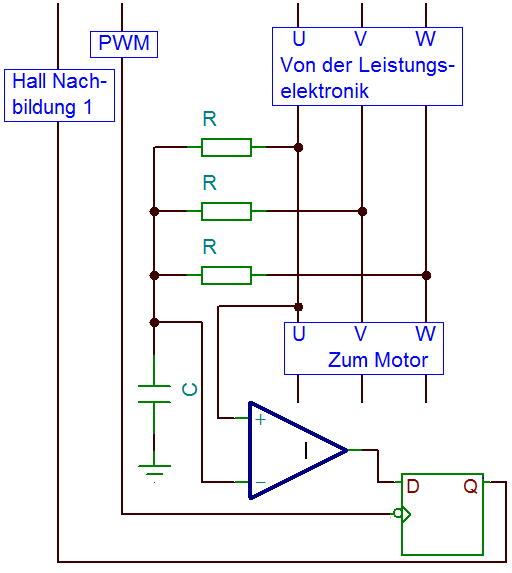
\includegraphics[scale=0.46]{\BLDCPath/Bilder/PrinzipDerRekonstruktion.png}
            \centering
            \caption[Schema des Rekonstruktionsprinzip]{Schema des Rekonstruktionsprinzip \cite{HSLU:Pluess}}
            \label{abb:PrinzipRekonstruktion}
        \end{wrapfigure}
    \fi
        In einem modifizierten Ansatz wird versucht, die Hallsensor-Signale 
        aus den Ansteuerungen des Motors zu gewinnen. Hierzu wird 
        eine Schaltung pro Phase benötigt, um die Nulldurchgänge beim 
        virtuellen Sternpunkt detektieren zu können. Die Abbildung 
        \ref{abb:PrinzipRekonstruktion} zeigt die Schaltung, mit der dieser Ansatz 
        realisiert werden kann. 
    \ifSTANDALONE
    	\begin{figure}[h!]
            \centering
            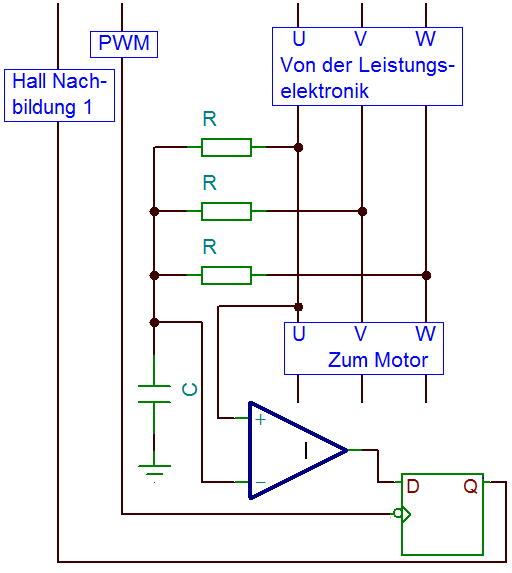
\includegraphics[scale=0.46]{\BLDCPath/Bilder/PrinzipDerRekonstruktion.png}
           	\caption{Schema des Rekonstruktionsprinzip \protect\cite{HSLU:Pluess}}
            \label{abb:PrinzipRekonstruktion}
        \end{figure}
    \fi
        Mit dem Flip-Flop aus Abbildung \ref{abb:PrinzipRekonstruktion} kann die PWM aus dem 
        Sensorsignal unterdrückt werden. Diese rekonstruierten 
        Hallsensor-Signale können direkt logisch verknüpft und genutzt 
        werden, um den Motor mit einer Dreiphasen-H-Brücke anzusteuern 
        \cite{HSLU:Pluess}. Anhand des zeitlichen Verlaufs, der aus Abbildung 
        \ref{abb:ZeitlicheAnsteuerungBrushlessMotor} zu entnehmen ist und der 
        Ansteuerung einer H-Brücke, ergibt sich die Wahrheitstabelle, die in 
        Tabelle \ref{abb:WahrheitstabelleAnsteuerung} ersichtlich ist. Das 
        Signal $U_h$ symbolisiert den Highside\footnote{Transistor, der gegen 
        die Versorgungsspannung schaltet. Typischerweise aufwendiger 
        anzusteuern, da am Gate eine Spannung von einigen Volt über der 
        Versorgungsspannung angelegt werden muss. }-Transistor der Phase U auf der 
        H-Brücke und die Spalte $U_l$ entspricht dem Lowside-Transistor.\\      
        
        \begin{table}[h!]
            \begin{tabular}{ccc||cc|cc|cc||c}
                 $H_1$ & $H_2$ & $H_3$ & $U_h$ & $U_l$ & $V_h$ & $V_l$ & $W_h$ & $W_l$ & Illegal\\
            \hline 0   &   0   &   0   &   0   &   0   &   0   &   0   &   0   &   0   &   1\\
                   0   &   0   &   1   &   0   &   0   &   0   &   1   &   1   &   0   &   0\\
                   0   &   1   &   0   &   0   &   1   &   1   &   0   &   0   &   0   &   0\\
                   0   &   1   &   1   &   0   &   1   &   0   &   0   &   1   &   0   &   0\\
                   1   &   0   &   0   &   1   &   0   &   0   &   0   &   0   &   1   &   0\\
                   1   &   0   &   1   &   1   &   0   &   0   &   1   &   0   &   0   &   0\\
                   1   &   1   &   0   &   0   &   0   &   1   &   0   &   0   &   1   &   0\\
                   1   &   1   &   1   &   0   &   0   &   0   &   0   &   0   &   0   &   1\\
            \end{tabular}
           	\centering
           	\caption{Wahrheitstabelle der Ansteuerung} 
            \label{abb:WahrheitstabelleAnsteuerung}
        \end{table}
        \parindent 0pt Die Tabelle in Abbildung 
        \ref{abb:WahrheitstabelleAnsteuerung} kann pro Signal zu folgenden 
        logischen Verknüpfung vereinfacht werden\\
        \\
    \ifSTANDALONE
        \begin{table}
            \centering
            \begin{tabular}{ccc}
                $U_h = H_1 \wedge \bar{H_2}$ & $V_h = H_2 \wedge \bar{H_3}$ & $W_h = \bar{H_1} \wedge H_3$\\
                $U_l = \bar{H_1} \wedge H_2$ & $V_l = \bar{H_2} \wedge H_3$ & $W_l = H_1 \wedge \bar{H_3}$
            \end{tabular}
        \end{table}
    \fi
    \ifEMBED
        \begin{tabular}{ccc}
            $U_h = H_1 \wedge \bar{H_2}$ & $V_h = H_2 \wedge \bar{H_3}$ & $W_h = \bar{H_1} \wedge H_3$\\
            $U_l = \bar{H_1} \wedge H_2$ & $V_l = \bar{H_2} \wedge H_3$ & $W_l = H_1 \wedge \bar{H_3}$
        \end{tabular}
    \fi
    \ifSTANDALONE
    \subsection{Ansteuerungshardware}
    \fi
    \ifEMBED
    \paragraph{Ansteuerungshardware}$~~$\vspace{2mm}\\
    \fi
        In Kapitel \ref{chap:VersuchsResultat} zeigten sich einige Punkte, die für ein eigenes Board 
        für die Brushless-Motoransteuerung sprechen. Auf diesem Board wird ein eigener Controller 
        eingesetzt, der als Kommunikationsschnittstelle SPI verwendet. Die benötigten Pins sind in 
        der Tabelle \ref{abb:SchnittstelleBrushlessBoard} ersichtlich. Der Controller wird benötigt, 
        um eine Zwangskommutierung vorzunehmen, um den Motor in eine Initialdrehung zu versetzen. 
        Sobald der Motor dreht, kann der neue Ansatz funktionieren. Weiter wird auf dem Controller eine 
        Regelung implementiert, um die Drehzahl des Motors zu regeln. Zusätzlich kann der Winkel 
        zwischen Detektion und Kommutierung angepasst werden, wenn dies notwendig ist.\\
        \\
        Die Kommunikation mit dem Controller soll über SPI geschehen. Darüber sollen die Solldrehzahl 
        und gegebenenfalls Parameter eingestellt werden können. Alle weiteren Schritte, wie die benötigte 
        Zwangskommutierung am Anfang und die Regelung, werden eigenständig vom Boardcontroller vorgenommen.
        %
        \begin{table}[h!]
            \begin{tabular}{ll}
                Pin     & Funktion \\
            \hline  SCK & Bustakt \\
                MISO    & Master in Slave out \\
                MOSI    & Master out Slave in \\
                CS      & Chip select \\
                Int     & Interrupt \\
                Reset   & Reset \\
            \end{tabular}
           	\centering
           	\caption{Schnittstelle des Brushless-Boards} 
            \label{abb:SchnittstelleBrushlessBoard}
        \end{table}

    \clearpage
    \ifSTANDALONE
\section{Prinziptest}
\fi
\ifEMBED
\subsubsection{Aufbaubeschreibung}
    \BLDCcollab \\
\fi
\ifEMBED
    \begin{wrapfigure}{r}{0.55\textwidth}
       	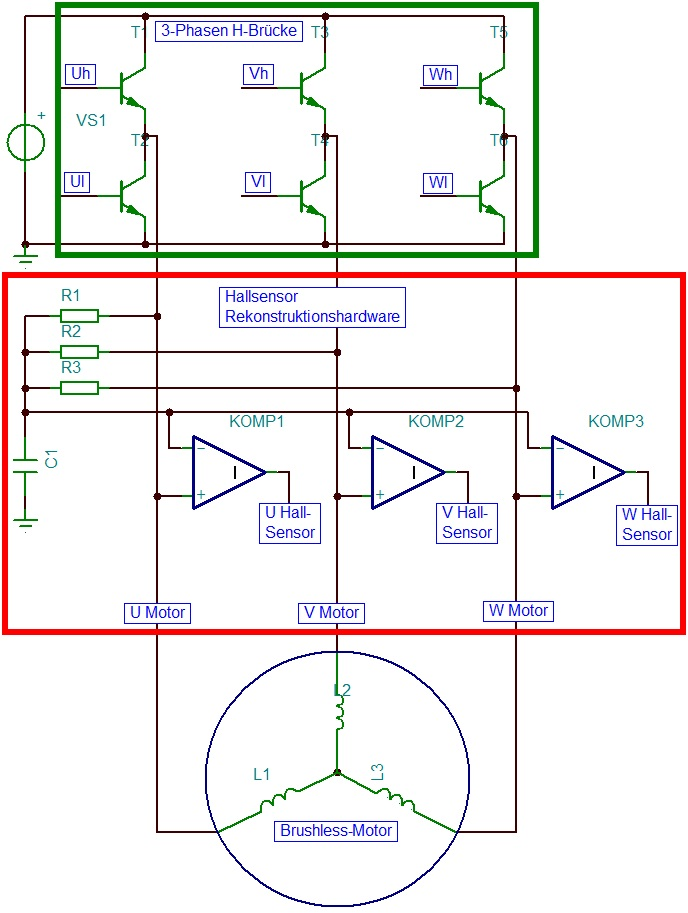
\includegraphics[scale=0.4]{\EtPath/Bilder/MotoransteuerungSchema.jpg}
       	\centering
       	\caption{Schema des Brushless-Versuchsaufbaus}
        \label{abb:MotoransteuerungSchema}
    \end{wrapfigure}
\fi
    Das Schema des Gesamtaufbaus des Tests ist in der Abbildung 
    \ref{abb:MotoransteuerungSchema} ersichtlich. Die 3-Phasen H-Brücke im 
    oberen grünen Rechteck wird direkt vom FPGA 
    \footnote{\textbf{F}ield-\textbf{P}rogrammable \textbf{G}ate 
    \textbf{A}rray} angesteuert. Die Hardware dieser Brücke ermöglicht eine 
    voll galvanisch getrennte Ansteuerung mit $3.3 V$ Logikpegeln. Diese 
    Brücke wurde zur Verfügung gestellt und direkt verwendet. Die 
    Rekonstruktion der Hallsensoren-Signale findet im rot markierten Teil des 
    Aufbaus statt. Dieser Part wird auf einer Laborplatte aufgebaut und 
    gelötet. Die so generierten Signale $U_{Hallsensor}$, $V_{Hallsensor}$, 
    $W_{Hallsensor}$ werden einem FPGA geliefert. Anhand dieser Signale 
    steuert das FPGA die H-Brücken-Transistoren mit den Signalen $U_h$, $U_l$, 
    $V_h$, $V_l$, $W_h$, $W_l$. Die im FPGA enthaltene Konfiguration besteht 
    aus simplen AND-Verknüpfungen, die die anliegenden Signale sehr schnell 
    und effizient verarbeiten können. Auf diese Weise ist es möglich, den 
    Motor sehr schnell anzusteuern.
    \ifSTANDALONE
    \begin{figure}[h!]
    	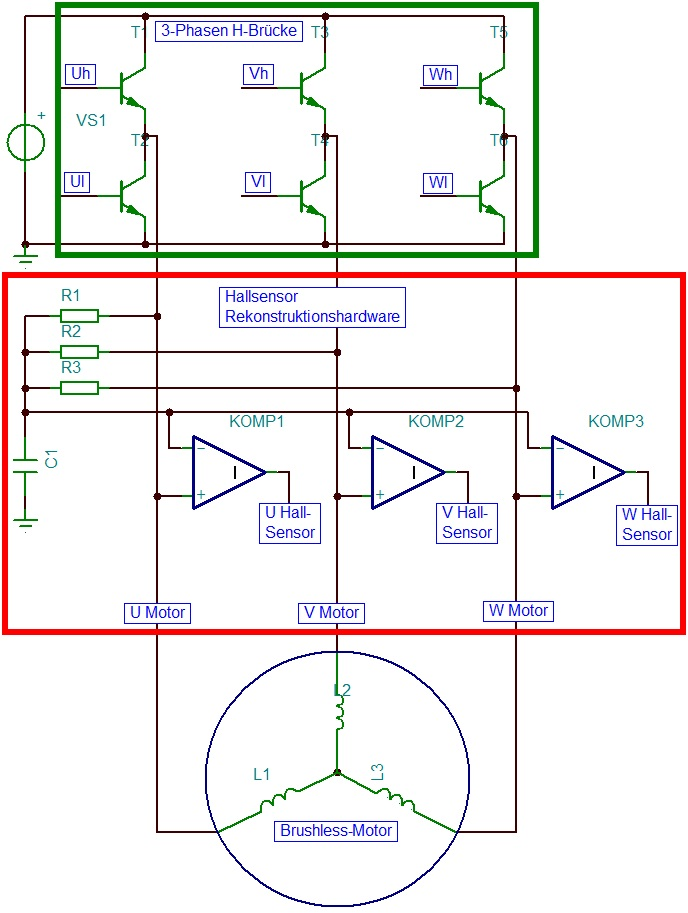
\includegraphics[scale=0.4]{\EtPath/Bilder/MotoransteuerungSchema.jpg}
       	\centering
       	\caption{Schema des Brushless-Versuchsaufbaus}
        \label{abb:MotoransteuerungSchema}
    \end{figure}
    \fi
    In der Abbildung \ref{abb:MessplatzAufbau} ist der gesamte Aufbau 
    abgebildet. Man beachte die markierten Felder. Am linken unteren Rand ist 
    der Motor befestigt. In der Mitte des Bildes ist die Hardware zur 
    Rekonstruktion der Hallsensoren-Signale.  Die generierten Signale werden 
    dem FPGA in der unteren rechten Ecke zugeführt. Diese Signale werden 
    logisch verknüpft und danach die sechs Signale generiert, um die H-Brücke 
    in der rechten oberen Hälfte anzusteuern.  Die H-Brücken wiederum treiben 
    den Motor an.
    \begin{figure}[h!]
    %\vspace{-16pt}
       	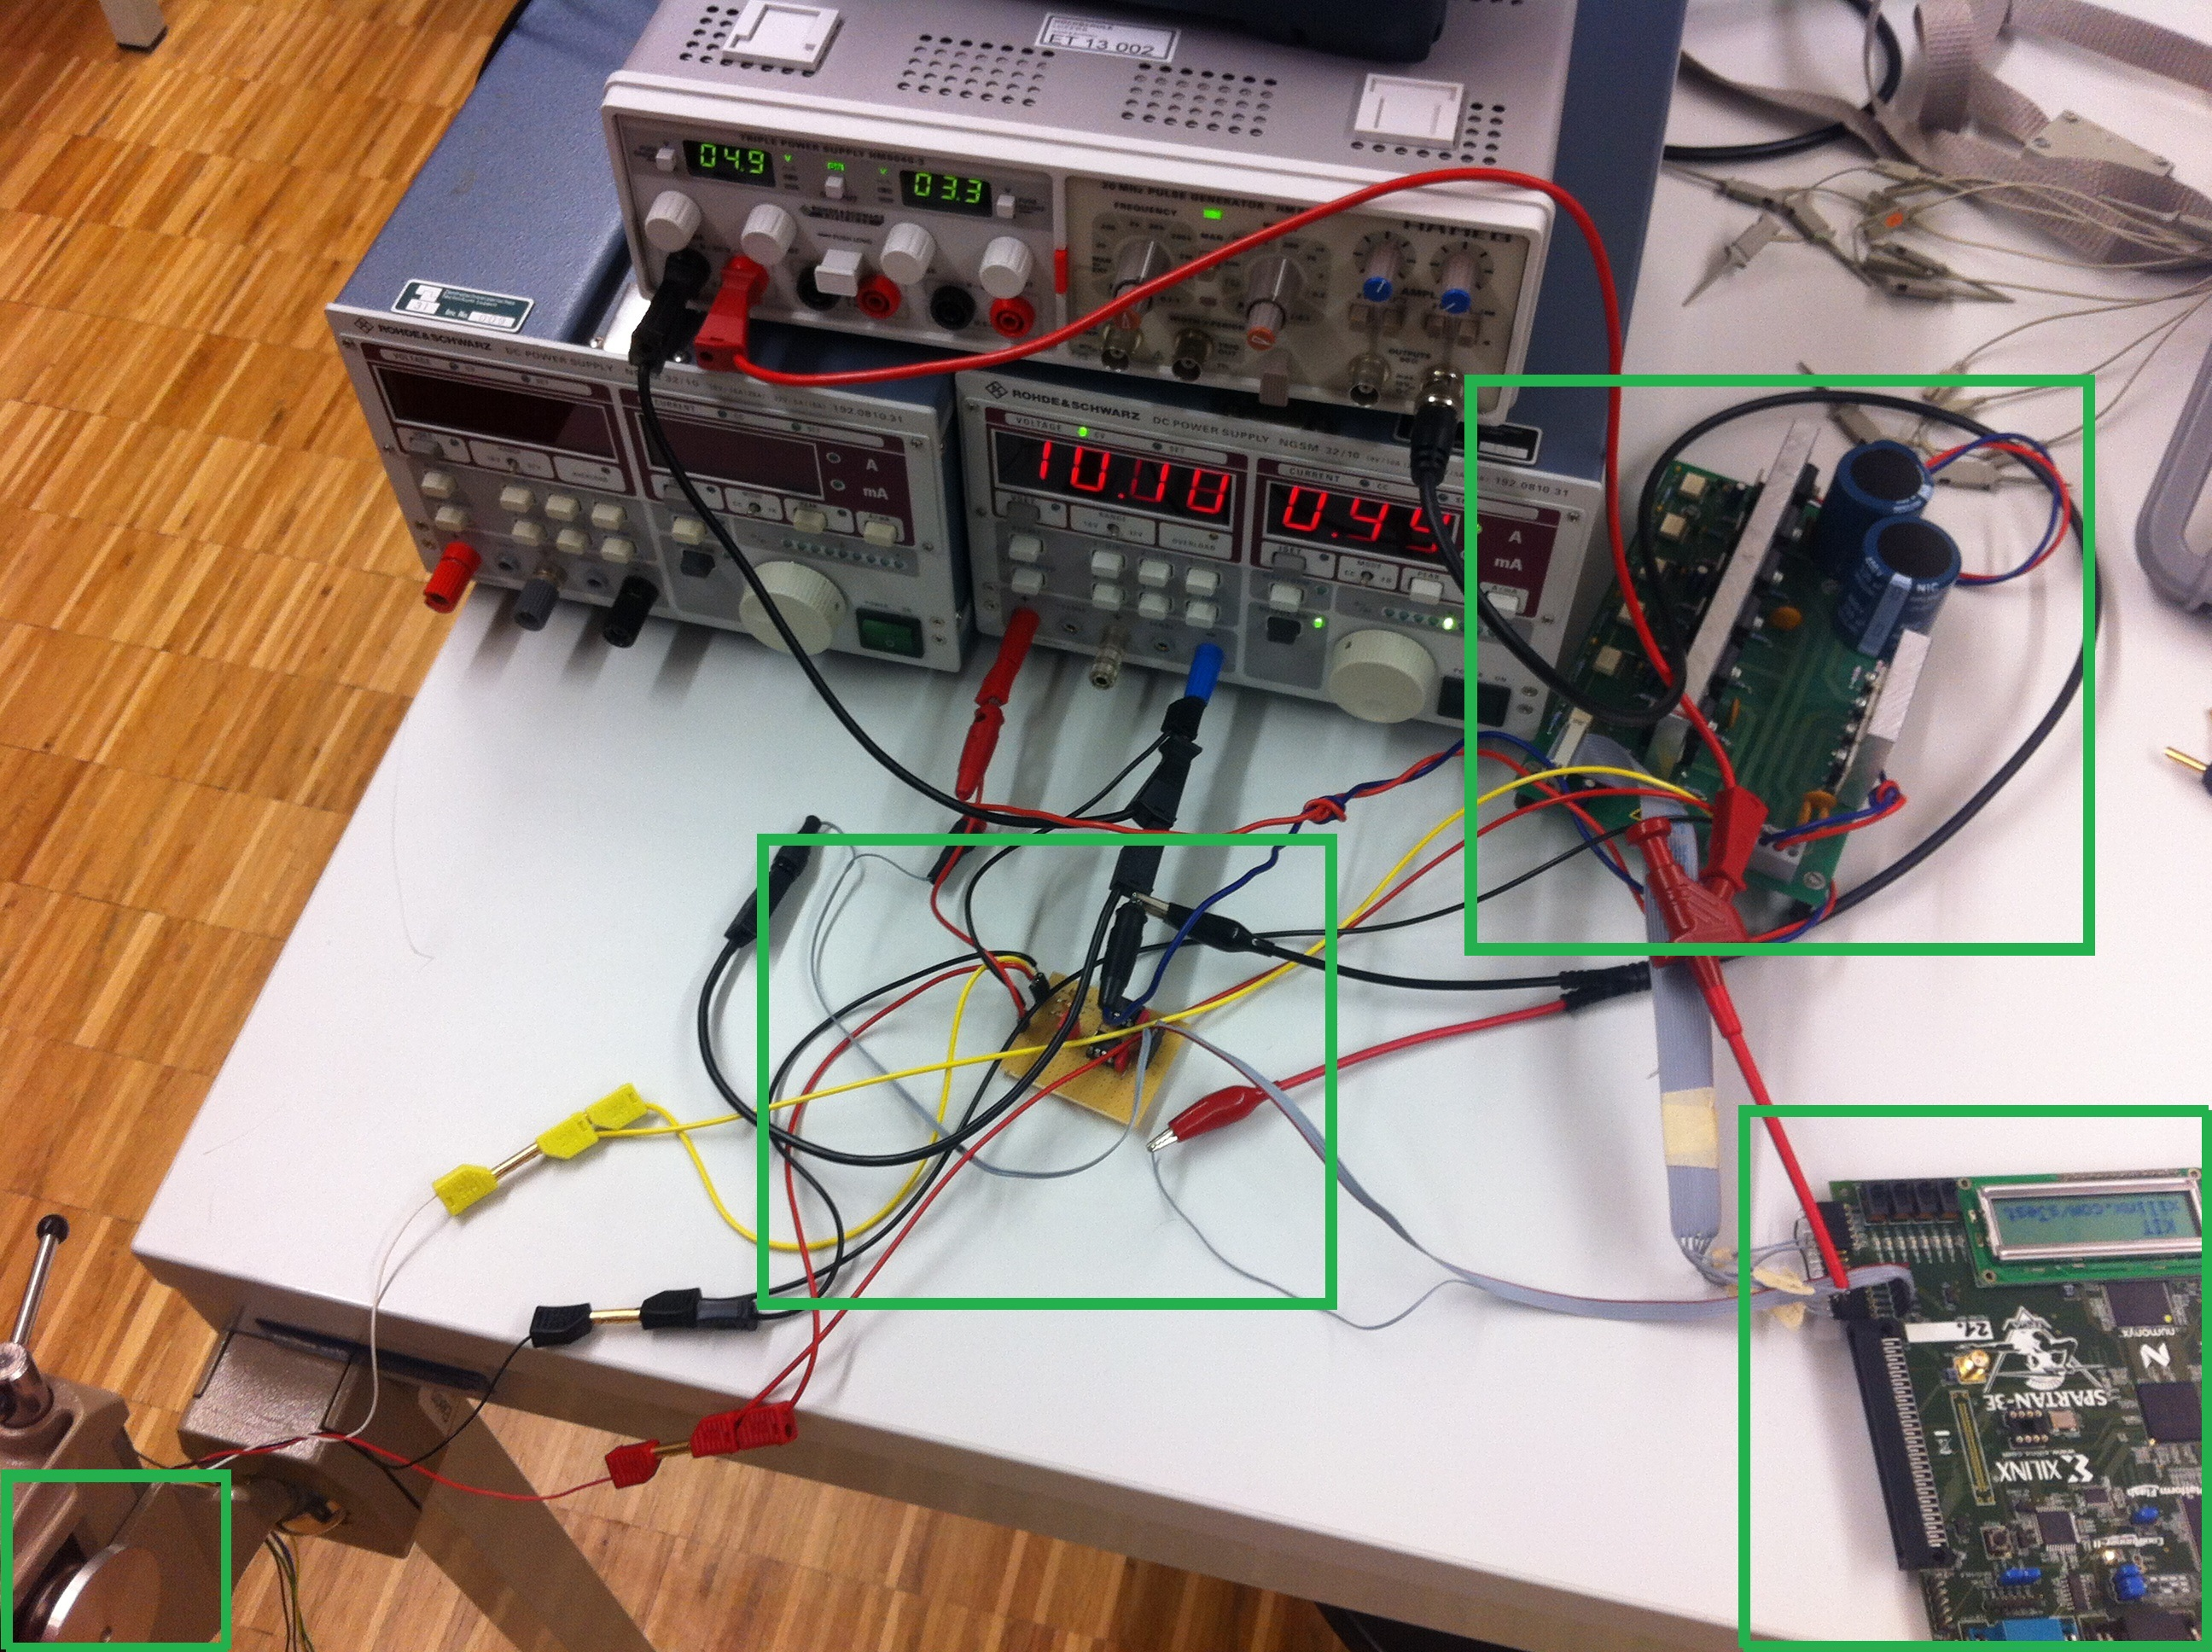
\includegraphics[width=0.9\textwidth]{\EtPath/Bilder/MessplatzAufbau.jpg}
       	\centering
       	\caption{Testaufbau} 
        \label{abb:MessplatzAufbau}
    %\vspace{-10pt}
    \end{figure}
    Die im FPGA enthaltene Logik basiert auf der Wahrheitstabelle, die in 
    Tabelle \ref{abb:WahrheitstabelleAnsteuerung} abgebildet ist.

\ifSTANDALONE
\subsection{Messmittel}
\fi
\ifEMBED
\newpage
\subsubsection{Messmittel}
\fi
    \begin{table}[h!]
        \centering
        \begin{zebratabular}{lll}
            \rowcolor{gray}
            Gerät &
                Typ &
                Nummer \\
            Speisegerät & 
                Rohde \& Schwarz NGSM 32/10 &
                Inv.-Nr. 009 \\
            Oszilloskop &
                Agilent MSO6052A &
                Inv.-Nr. 48; S/N: MY44001903 \\
            Mainframe &
                Hameg HM8001-2 &
                SN: 059520046 \\
            Speisegerät &
                Hameg HM8040-3 &
                SN: 015405014 \\
            Pulsgenerator &
                Hameg HM8035 &
                Inv.-Nr. 44 \\
        \end{zebratabular}
        \caption{Messmittel des Versuchsaufbaus}
    \end{table}

\ifSTANDALONE
\subsection{Resultat}
\label{chap:VersuchsResultat}
\fi
\ifEMBED
\subsubsection{Resultat}
\label{chap:VersuchsResultat}
\fi
Mit dem beschriebenen Aufbau konnte ein BLDC-Motor erfolgreich angesteuert 
werden. Wie in Abbildung \ref{abb:MessplatzAufbau} am linken unteren Rand zu 
erkennen ist, ist an der Motorwelle eine Aluminiumplatte montiert. Mit dieser 
und eines Magneten konnte der Motor mittels einer Wirbelstrombremse belastet 
werden. Auf diese weise konnte rund $120 W$ elektrische Leistung umgesetzt 
werden. Dabei stellte sich heraus, dass die PWM nachgeregelt werden muss, wenn 
eine Last getrieben wird. Weiter bietet der Aufbau, wie er getestet wurde 
keine Möglichkeit den Motor ohne äussere Manipulation zu starten.\\
\\
Diese beiden Tatsachen sprechen dafür, dass das Prinzip grundsätzlich 
funktioniert. Für die Realisierung würde sich ein eigenes Board anbieten, auf 
dem ein eigener Controller die Regelung und die Zwangskommutierung beim 
Starten des Motors übernimmt.

    \clearpage
    \ifSTANDALONE
\section{Hardware}
\fi
\ifEMBED
\subsubsection{Hardware}
\label{sec:ET_Hardware}
\fi
\ifSTANDALONE
\subsection{Übersicht}
\fi
\ifEMBED
\paragraph{Übersicht}$~~$\vspace{2mm}\\
\fi
Der Aufbau der Ansteuerung der BLDC-Motoren ist als Blockschaltbild in Abbildung 
\ref{abb:BlockschaltbildBLDC} ersichtlich.\\
\begin{figure}[h!]
   	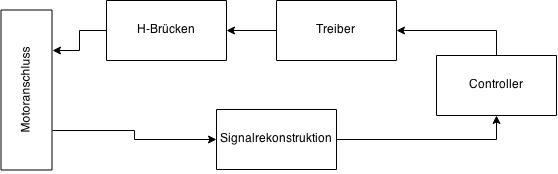
\includegraphics[width=0.8\textwidth,clip,trim=0mm 0mm 0mm 0mm]
   	{\EtPath/Bilder/Blockschaltbild_BLDC.jpg}
   	\centering
   	\caption{Blockschaltbild des BLDC-Boards}
   	\label{abb:BlockschaltbildBLDC}
\end{figure}\\
In der Abbildung \ref{abb:BlockschaltbildBLDCPhoto} ist die Realisierung der Blöcke ersichtlich. 
Dabei ist der erste Kasten der Anschluss des Motors, der zweite die H-Brücken, der dritte der 
Treiber, der vierte die Signalrekonstruktion und der fünfte Teil ist der Controller, auf dem 
die Firmware läuft. Das ganze Schema des Boards ist im Anhang \ref{apx:Schema_BLDC} angefügt.
\begin{figure}[h!]
   	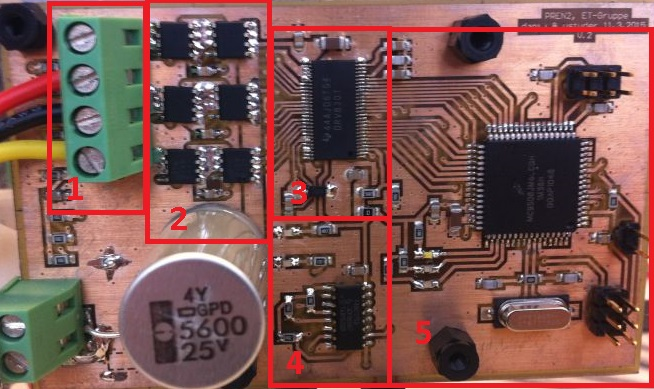
\includegraphics[width=0.8\textwidth,clip,trim=0mm 0mm 0mm 0mm]
   	{\EtPath/Bilder/BLDC-BoardBloecke.jpg}
   	\centering
   	\caption{Blockschaltbild des BLDC-Boards}
   	\label{abb:BlockschaltbildBLDCPhoto}
\end{figure}

\ifSTANDALONE
\subsection{Kommutierung}
\fi
\ifEMBED
\paragraph{Kommutierung}$~~$\vspace{2mm}\\
\fi
\begin{figure}[h!]
   	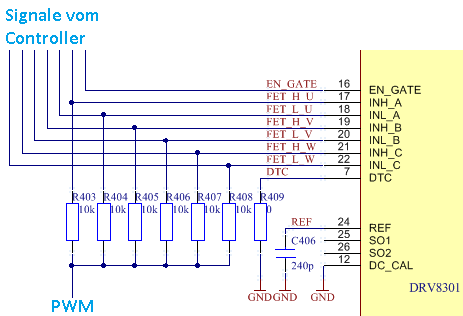
\includegraphics[width=.6\textwidth,clip,trim=0mm 0mm 0mm 0mm]
   	{\EtPath/Bilder/Schema_PWM.png}
   	\centering
   	\caption{Schema-Ausschnitt der PWM-Verteilung}
   	\label{abb:SchemaKommutierung}
\end{figure}
Der Motor wird mit drei Halbbrücken kommutiert. Für die Ansteuerung der 
MOSFET\footnote{\textbf{M}etal \textbf{O}xide \textbf{S}emiconductor 
\textbf{F}ield \textbf{E}ffect \textbf{T}ransistor} 
wird ein Predriver DRV8301 von Texas Instruments eingesetzt. Die Halbbrücken 
werden einzeln vom Controller geschalten. Damit nur ein PWM-Signal erzeugt 
werden muss, sind die Ansteuerleitungen mittels Widerständen mit dem 
PWM-Signal verbunden. (siehe Abbildung \ref{abb:SchemaKommutierung}) 
Sind die Ansteuerungen vom Controller nicht aktiv 
getrieben, liegt die PWM an. Die Konfiguration der Predrivers erfolgt über SPI. 

\ifSTANDALONE
\subsection{Phasendetektion}
\fi
\ifEMBED
\paragraph{Phasendetektion}$~~$\vspace{2mm}\\
\fi
\begin{figure}[h!]
    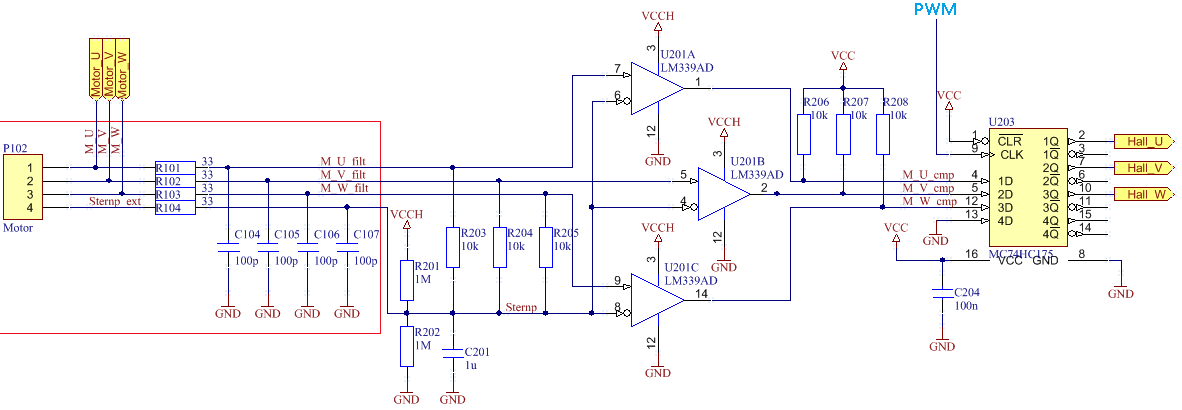
\includegraphics[width=1\textwidth,clip,trim=0mm 0mm 0mm 0mm]
   	{\EtPath/Bilder/Schema_Phasendetektion.png}
   	\centering
   	\caption{Schema-Ausschnitt der Phasendetektion}
   	\label{abb:SchemaPhasenDetektion}
\end{figure}
Die Phasendetektion besteht aus Sternpunktnachbildung (R201 - R205 in 
Abbildung \ref{abb:SchemaPhasenDetektion}), Komparator (U201) und 
Synchronisation (U203). Die Sternpunktnachbildung erzeugt einen virtuellen 
Sternpunkt mit Hilfe eines Widerstandsnetzwerkes und eines Tiefpassfilters. 
Besitzt der verwendete Motor einen herausgeführten Sternpunkt, so kann auch 
dieser verwendet werden. Die einzelnen Phasenspannungen werden mit diesem 
virtuellen Sternpunkt verglichen. Mit einem Flipflop wird das Signal mit der 
PWM synchronisiert. 
\ifEMBED 
Das Konzept wurde im PREN1 \cite{Team32:Doku} ausführlich beschrieben.
\fi

\ifSTANDALONE
\subsection{Controller}
\fi
\ifEMBED
\paragraph{Controller}$~~$\vspace{2mm}\\
\fi
Als Controller kommt ein HC9S08JM60 der Firma Freescale zum Einsatz. Der Takt 
wird mittels Quarz mit 12\si{\mega\hertz} erzeugt. Um den aktuellen Betriebsszustand 
anzuzeigen, stehen drei LED zur Verfügung. 

\ifSTANDALONE
\subsection{Speisung}
\fi
\ifEMBED
\paragraph{Speisung}$~~$\vspace{2mm}\\
\fi
Die Eingangsspannung wird mittels eines optional bestückbaren Filters von 
Murata gefiltert. Der Predriver wird direkt mit dieser gefilterten Speisung 
betrieben. Mit dem im Predriver integrierten Step-Down-Converter wird eine 
Spannung von 3.3\si{\volt} erzeugt. Für Varianten mit hoher Betriebsspannung (>30\si{\volt}) 
wird der Komparator der Phasendetektion über einen diskret aufgebauten 
Spannungsregler mit einer Spannung von 30\si{\volt} versorgt. 


    \clearpage
    \ifSTANDALONE
\section{Firmware}
\fi
\ifEMBED
\subsubsection{Firmware}
\label{sec:ET_Firmware}
\fi
\ifSTANDALONE
\subsection{Übersicht}
\fi
\ifEMBED
\paragraph{Übersicht}$~~$\vspace{2mm}\\
\fi
Die Firmware des Boards erfüllt mehrere Aufgaben. Während dem Anfahren des Motors realisiert
sie die Zwangskommutierung, im Nennbetrieb regelt sie die Drehzahl des
Motors. Sobald der Motor in Betrieb ist, wir die Kommutierung mittes Interrupts hardwaremässig
realisiert.
\ifSTANDALONE
\subsection{Takt}
\fi
\ifEMBED
\paragraph{Takt}$~~$\vspace{2mm}\\
\fi
Der Referenztakt wird durch einen Quarz mit einer Frequenz von 
12\si{\mega\hertz} erzeugt.  Dieser Takt dient als Referenztakt für die PLL\footnote{phase-locked loop, eine elektronische Schaltung, die die Phasenlage und Frequenz beeinflussen kann} 
des HS9S08JM60. Dazu wird er durch acht geteilt um im erlaubten 
Bereich\footnote{Die Frequenz des Eingangssignals der PLL muss im Bereich 1 
\ldots 2\si{\mega\hertz} liegen. \cite[p.  195]{Datasheet:HCS08}} für die PLL 
zu liegen. In der PLL wird der Takt mit 32 multipliziert. Dies ergibt einen 
CPU Takt von 48\si{\mega\hertz}. Da der Bustakt der Hälfte des CPUtakts 
entspricht, weist dieser eine Frequenz von 24\si{\mega\hertz} auf.  Der 
Externe Takt (16\si{\mega\hertz}) wird zusätzlich als externer Referenztakt 
zur Verfügung gestellt und vom RTC verwendet.  (siehe auch Abschnitt 
\ref{sec:rtc} \nameref{sec:rtc})

\ifSTANDALONE
\subsection{RTC}
\fi
\ifEMBED
\paragraph{RTC}$~~$\vspace{2mm}\\
\fi
\label{sec:rtc}
Um regelmässig abzuarbeitende Aufgaben zu steuern, wird ein entsprechender 
Takt benötigt. Dafür wird der RTC\footnote{\textbf{R}eal \textbf{T}ime 
\textbf{Counter}} verwendet. Dieser verwendet als Takt den externen 
Referenztakt mit einer Frequenz von 16\si{\mega\hertz}. Dieser wird mit dem 
Prescaler auf eine Frequenz von 16\si{\kilo\hertz} geteilt. Über das Modulo 
Register kann eine Periodendauer im Bereich 62.5\si{\micro\second} \ldots 
16\si{\milli\second} eingestellt werden. Es wird zunächst eine Periodendauer 
von 1\si{\milli\second} verwendet. In der ISR\footnote{\textbf{I}nterrupt 
\textbf{S}ervice \textbf{Routine}} wird ein Flag gesetzt, welches in der 
Hauptschlaufe abgefragt wird. 

\ifSTANDALONE
\subsection{PWM}
\fi
\ifEMBED
\paragraph{PWM}$~~$\vspace{2mm}\\
\fi
Mit der PWM werden 
die Ausgangsstufen angesteuert. Über das Puls - Pausenverhältnis wird die 
Leistung eingestellt. Damit diese Ansteuerung jedoch nicht hörbar wird, muss 
der Motor mit einer PWM Frequenz oberhalb des hörbaren Frequenzbereichs des 
Menschen angesteuert werden. Es wird eine Frequenz von 24\si{\kilo\hertz} 
verwendet.  Für das Erzeugen der PWM wird der Timer TPM2 verwendet. 

\ifSTANDALONE
\subsection{Kommutierungsverzögerung / Zeitmessung}
\fi
\ifEMBED
\paragraph{Kommutierungsverzögerung / Zeitmessung}$~~$\vspace{2mm}\\
\fi
Um den exakten Kommutierungszeitpunkt einstellen zu können und um die Zeit 
zwischen zwei Kommutierungen zu messen, wird ein weiterer Timer benötigt. Dafür 
wird TPM1 benutzt. Als Taktquelle für den Timer wird der Bustakt mit einer 
Frequenz von 24\si{\mega\hertz} verwendet. Dieser wird mit dem maximal möglichen 
Prescaler von 128 geteilt. Dies ergibt eine Frequenz von 187.5\si{\kilo\hertz} 
und eine Auflösung von 5.33\si{\micro\second}. Damit ist eine maximale 
Messdauer von 349.5\si{\milli\second} möglich. 

\ifSTANDALONE
\subsection{Kommutierung}
\fi
\ifEMBED
\paragraph{Kommutierung}$~~$\vspace{2mm}\\
\fi
Die Kommutierung wird mit dem Timer TPM1 realisiert. Bei der 
Zwangskommutierung und bei der Wiedergabe von Tönen wird der Kanal 0 
verwendet. Dieser liest aus globalen Registern die Zeitdauer für die 
Kommutierung aus. In der ISR wird eine Zustandsmaschine ausgeführt. Diese 
steuert die drei Phasen des Motors entsprechend dem aktuellen Zustand an. Bei 
Autokommutierung wird die Zustandsmaschine basierend auf den Signalen aus der 
Phasendetektion (siehe Abschnitt \ref{sec:phase_det}) ausgeführt. Dazu kommen 
die Kanäle 3 bis 5 zum Einsatz, welche als Input Capture konfiguriert sind. So 
kann parallel zur Kommutierung die Drehzahl des Motors gemessen werden. 

\ifSTANDALONE
\subsection{Kommunikation zum Host}
\fi
\ifEMBED
\paragraph{Kommunikation zum Host}$~~$\vspace{2mm}\\
\fi
Zur Interaktion mit dem BLDC-Board wird die SPI1-Schnittstelle des \si{\micro}C verwendet. Dabei
ist das SPI-Interface im 8 Bit Mode mit LSB-First konfiguriert. Zusätzlich zu dieser Schnittstelle
ist eine IRQ-Leitung vorhanden, mit der das BLDC-Board den Host triggern kann, um auf ein Problem 
hinzuweisen. Die Steckerbelegung ist in Tabelle \ref{tab:SPI_stecker} ersichtlich.

\begin{table}[h!]
    \begin{zebratabular}{p{0.10\textwidth}p{0.06\textwidth}}
    \rowcolor{gray} Pin & Name\\
    1 & GND\\
    2 & MISO\\
    3 & CS\\
    4 & MOSI\\
    5 & CLK\\
    6 & IRQ\\
    \end{zebratabular}
    \centering
    \caption{Steckerbelegung der SPI-Schnittstelle}
    \label{tab:SPI_stecker}
\end{table}
Die Kommunikation zwischen BLDC-Board und Host funktioniert über ein Protokoll zur Interaktion. Die 
Spezifikation dieses Protokolls ist in der Tabelle \ref{tab:Spi_Int_Table} ersichtlich. Das obere Nibble des
CMD's\footnote{Command-Byte, ein spezielles Byte, das zur Signalisation von Befehlen verwendet wird} 
enthält den Befehl und das untere Nibble die Anzahl Argumente, die zum CMD gehören.
Wenn das untere Nibble \verb!0xF! ist, wird die Länge der Übertragung im nächsten Byte signalisiert.

\ifSTANDALONE
    \begin{table}[h!]
    \begin{zebratabular}{p{0.12\textwidth}p{0.06\textwidth}p{0.35\textwidth}p{0.4\textwidth}}
\fi
    \ifEMBED
    \begin{zebralongtable}{p{0.12\textwidth}p{0.06\textwidth}p{0.35\textwidth}p{0.4\textwidth}}
        \caption{Kommunikationsprotokoll}
        \endlastfoot
\fi
    \rowcolor{gray} Name & Wert & Beschreibung & Parameter\\
    Dummy &
        \verb!0x00! & 
        Byte das benötigt wird, um zu clocken für die Übertragung von Argumenten &
        \\
    Start &
        \verb!0x10! & 
        Startet den Motor &
        \\
    Stop &
        \verb!0x20! & 
        Stoppt den Motor &
        \\
    setRPM &
        \verb!0x32! & 
        16 Bit Zahl um die Drehzahl einzustellen & 
        1. Byte = High-Byte\newline 
        2. Byte = Low-Byte\\
    setVoltage &
        \verb!0x42! & 
        $U_{GS}$ der FET's. & 1. Byte = Spannungswert-High-Byte\newline 
                              2. Byte = Spannungswert-Low-Byte\\
    setCurrent &
        \verb!0x51! & 
        Wert der Strombegrenzung. Der Stromwert ergibt sich nach der Formel $Current = Wert \cdot 10$ &
        $Registerwert = \frac{Sollwert\; in \;[mA]}{10} $\\
    getStatus &
        \verb!0x64! & 
        Gibt der Board-Status zurück &
        1. Byte = Motor-Status\newline
        2. Byte = Fehler-Code\newline
        3. Byte = RPM-High-Byte\newline
        4. Byte = RPM-Low-Byte\\
    areYouAlive &
        \verb!0x71! & 
        Damit kann die Kommunikation und das BLDC-Board testen &
        Das BLDC-Board gibt \verb!0x55! zurück\\
    setPwm &
        \verb!0x81! & 
        Damit kann die PWM des Motors eingestllt werden &
        PWM-Wert im Bereich 1-100 \% \\
    startMessung Param &
        \verb!0xC3! & 
        Messung parametrisiert starten &
        1. Byte = Pulsdauer\newline
        2. Byte = RPM-High-Byte\newline
        3. Byte = RPM-Low-Byte\\
    startMessung &
        \verb!0xD0! & 
        Messung mit einem Schritt starten &
        \\
    getMessung &
        \verb!0xEF! & 
        gibt die gespeicherte Messung zurück &
        1. Byte = Länge\newline
        2. - n. Byte = Daten der Messung
\ifSTANDALONE
    \end{zebratabular}
    \caption{Kommunikationsprotokoll}
    \label{tab:Spi_Int_Table}
    \end{table}
\fi
\ifEMBED
    \label{tab:Spi_Int_Table}
    \end{zebralongtable}
\fi

\ifSTANDALONE
\subsection{Regler}
\fi
\ifEMBED
\paragraph{Regler}$~~$\vspace{2mm}\\
\fi
In der Software ist ein PID-Regler mit Vorsteuerung implementiert. Dies ist im 
Blockschema in der Abbildung \ref{fig:BlockschemaRegler} abgebildet. Je nach 
Wahl der Parameter $P$, $I$, $D$ und $F_{\text{Vorsteuerung}}$, können nur einzelne Teile 
des Reglers verwendet werden. 
\ifSTANDALONE
Auf diese Weise kann zum Beispiel ein PI-Regler realisiert werden. 
\fi 
\ifEMBED
Während der Testphase, siehe Testbericht in Kapitel \ref{sec:ParameterSuche}, 
stellte sich heraus, dass ein reiner PI-Regler ohne Vorsteuerung den 
Anforderungen am besten entsprechen. somit sind die Parameter $D = 0$ und 
$F_{\text{Vorsteuerung}} = 0$.
\fi
Als Feedback wird die Zeit, die für die Kommutierung bereits besprochen wurde, 
verwendet. Damit kurzfristige Unregelmässigkeiten gedämpft werden, wird das 
Feedback durch ein FIR-Filter\footnote{Finite Impulse Response Filter, Ein 
Filter mit garantierter endlicher Antwort auf einen Impuls} gefiltert. Der 
Ausgang dieses Filters wird mittels eines Korrekturfaktor in RPM umgerechnet. 
Dieser Wert wird mit der Sollgrösse verrechnet und dem Regler zugeführt.
\tikzstyle{crosspoint}   = [circle, minimum size=0.15cm, inner sep=0pt, draw=black, fill=black]
\tikzstyle{sumpoint}     = [circle, draw=black]
\tikzstyle{controlblock} = [rectangle, rounded corners, minimum width=1.5cm, minimum height=1cm, draw=black]
\begin{figure}[h!]
    \centering
    \ifSTANDALONE
    \begin{tikzpicture}[node distance=2.0cm]
    \fi 
    \ifEMBED
        \begin{tikzpicture}[node distance=1.85cm]
    \fi
        \node (soll)    []                                  {Sollwert};
        \node (in)      [crosspoint, right of=soll]         {};
        \node (diff)    [sumpoint, right of=in]             {};
        \node (control) [controlblock, right of=diff]       {PID-Regler};
        \node (sum1)    [sumpoint, right of=control]        {};
        \node (path1)   [controlblock, right of=sum1]       {Strecke};
        \node (sum2)    [sumpoint, right of=path1]          {};
        \node (feedback)[crosspoint, right of=sum2]         {};
        \node (ist)     [right of=feedback]                 {Istwert};
        \node (moment)  [above of=sum2]                     {Störgrösse (Tennisball)};
        \node (fir)     [controlblock, below of=path1]      {FIR-Filter};
        \node (forward) [controlblock, above of=control]    {Vorsteuerung};
        \draw[thick, ->] (soll)     -- (diff) node[above left] {$+$};;
        \draw[thick, ->] (diff)     -- node[above] {e} (control);
        \draw[thick, ->] (control)  -- (sum1) node[below left] {$+$};
        \draw[thick, ->] (sum1)     -- (path1);
        \draw[thick, ->] (path1)    -- (sum2) node[below left] {$+$};
        \draw[thick, ->] (sum2)     -- (ist);
        \draw[thick, ->] (moment)   -- (sum2) node[above right] {$+$};
        \draw[thick, ->] (feedback) |- (fir);
        \draw[thick, ->] (fir)      -| (diff) node[below right] {$-$};
        \draw[thick, ->] (in)       |- (forward);
        \draw[thick, ->] (forward)  -| (sum1) node[above right] {$+$};
    \end{tikzpicture}
    \caption{Blockschema der Regelung}
    \label{fig:BlockschemaRegler}
\end{figure}


    \clearpage
    \ifSTANDALONE
\section{Fallback}
\fi
\ifEMBED
\subsubsection{Fallback}
\fi
Ist der Einsatz des vorgesehenen BLDC-Treibers nicht möglich, so muss eine
alternative Ansteuerung erfolgen. Eine solche kann mit einer handelsüblichen
Steuerungen aus dem Modellbau erfolgen. Eine solche BLDC-Steuerung ist per
PWM angesteuert, wobei die im Modellbau üblichen Signale gelten, wie in der
Abbildung \ref{fig:rc-pwm} dargestellt.

\begin{figure}[h!]
	\centering
	\begin{tikzpicture}
		% Achsen
		\draw[->] (-0.25,0) -- (10,0) node[anchor=north] {$t$};
		\draw[->] (0,-0.25) -- (0,3) node[anchor=west] {$u$};
		% Signal
		\draw[-,red,thick] (0,0) -- (1,0) -- (1,2) -- (2,2) -- 
			(2,0) -- (7,0) -- (7,2) -- (8,2) -- (8,0) -- (9,0);
		% Zeiten
		\draw[<->] (1,1.5) -- (7,1.5) node[midway, above] {$T=20$ms};
		\draw[<->] (1,0.5) -- (2,0.5) node[right] {$1$ms$ \leq t_{ON} \leq 2$ms};
	\end{tikzpicture}
	\caption{Signalverlauf eines typischen Modellbau-PWM Signals}
	\label{fig:rc-pwm}
\end{figure}

Der Einsatz von Modellbausteuerungen für BLDC-Motoren erfordert ein
Feedback der Drehzahl, da diese lediglich eine Steuerung darstellen. Die
Drehzahlregelung muss über eine externe Einheit erfolgen, beispielsweise einen
Mikrocontroller. Solche BLDC-Steuerungen werden im Modellbau typischerweise als
\emph{Regler} vertrieben und sind auch für hohe Leistungen durchaus preiswert.

\ifSTANDALONE
\subsection{Konzeptbeschreibung}
\fi
\ifEMBED
%\newpage
\paragraph{Konzeptbeschreibung}$~~$\vspace{2mm}\\
\fi
Um eine Regelung der Drehzahl des BLDC-Motors zu ermöglichen, bedarf es eines
Feebacks, welches die Drehzahl wiedergibt. Dies ist mit einem
Hall-Effekt-Schalter zu realisieren. Dieser reagiert auf die Magnetfelder,
welche durch Magnete auf dem Rotationskörper gegeben sind. Aus solch einem
Aufbau resultiert ein Feedback, welches mit Impulsen einen Segmentdurchlauf
des Rotationskörpers wiedergibt, wie in Abbildung \ref{fig:fallback-sketch}
dargestellt.
\begin{figure}[h!]
	\centering
	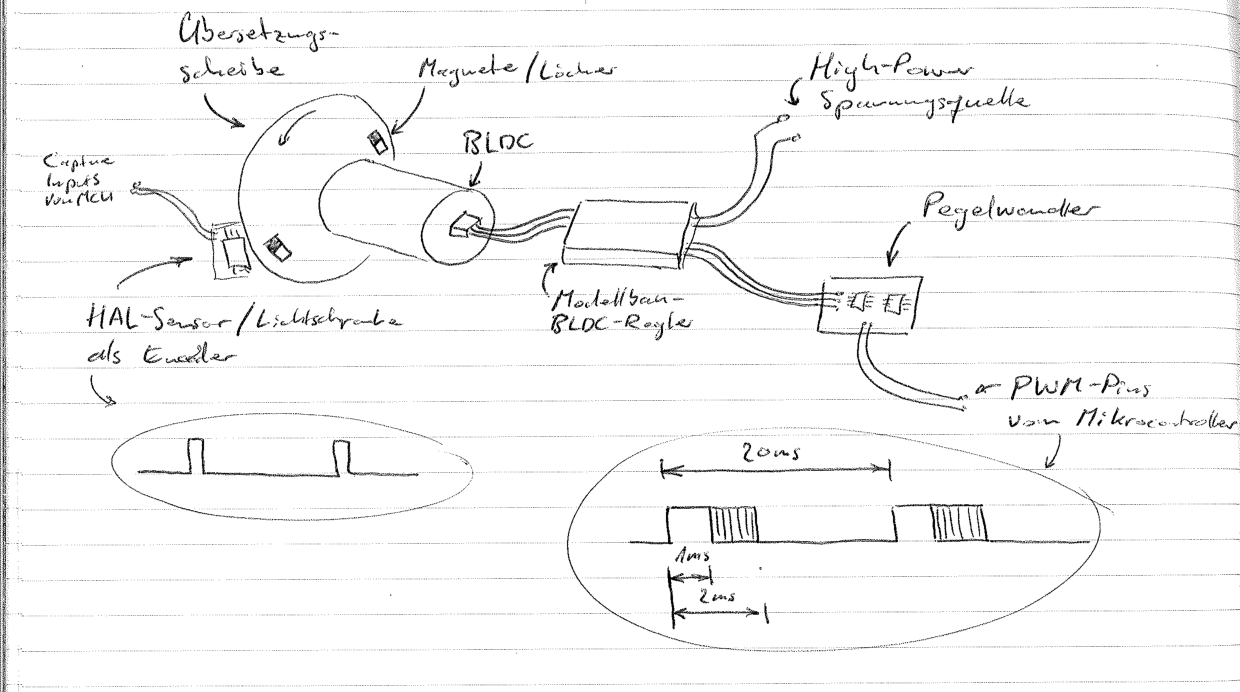
\includegraphics[width=0.8\textwidth]{\EtPath/Bilder/fallback_sketch_1.pdf}
	\caption{Erste Skizze des Fallback-Konzepts}
	\label{fig:fallback-sketch}
\end{figure}
Dieses Feedback wird mittels eines Mikrocontrollers ausgewertet und regelt
damit den Input der Steuerung mit dem PWM-Signal beziehungsweise der Impulsdauer.
Das Einlesen einer Flanke, die Zeitmessung bis zur nächsten Flanke und die
Stellung eines PWM-Signals, sind Tasks welche übliche Mikrocontroller direkt
durch ihre Peripherie-Module ausführen können. Dies ermöglicht eine einfache
Adaption in ein bestehendes Modell, denn es werden lediglich zwei Timer-IO
für diesen Fallback verwendet. Je nach Mikrocontroller ist ein Pegelwandler
für die PWM-Signale notwendig.

    \clearpage
    \ifSTANDALONE
\section{Encoder \& Drehzahlgeber}
\fi
\ifEMBED
\subsubsection{Encoder \& Drehzahlgeber}
\fi

Die vorgesehenen Motorfunktionen verlangen lediglich beim Brushlessmotor
nach einem Feedback über die Rotation des Motors, da der Schrittmotor
definiert und fein granuliert betrieben wird. Der Gleichstrommotor stellt
keinerlei Ansprüche, weder an die Drehzahl, noch an die Position.

Encoder sind relativ teuer und der Einsatz des Brushlessmotors verlangt
lediglich nach einem Feedback zur Rotation beziehungsweise Winkelgeschwindigkeit.
Die absolute oder relative Position ist für die Anwendung nicht von
Bedeutung. Somit lässt sich ein einfaches Feedback vorsehen, für die
Regelung der Drehzahl mit optischen oder magnetischen Elementen.
\ifSTANDALONE
\begin{figure}[h!]
	\centering
	\begin{tikzpicture}
		% Koordinaten
		\draw[->] (-0.5, 0) -- (8, 0) node[anchor=north] {$t$};
		\draw[->] (0, -1.5) -- (0, 3) node[anchor=east] {$u,\varphi$};
		% Rotation
		\draw[blue] (0,0) sin (1,1) cos (2,0) sin (3,-1) cos (4,0)
			sin (5,1) cos (6,0) sin (7,-1)
			node[right] {$\varphi$};
		% Signal
		\draw[-, thick, red]
			(0,0) -- (0.8,0) -- (0.8,2) -- (1.2,2) -- (1.2,0) -- 
			(4.8,0) -- (4.8,2) -- (5.2,2) -- (5.2,0) -- (7.5,0);
		% Messung
		\draw[<->] (0.8,1.5) -- (4.8,1.5) node[midway, above] {$t_{r}$};
	\end{tikzpicture}
	\caption{Vereinfachtes Puls-Feedback eines Hall-Effekt-Schalters}
	\label{fig:hall-effekt-schalter}
\end{figure}
\fi
\ifEMBED
\begin{figure}[h!]
	\centering
	\begin{tikzpicture}
		% Koordinaten
		\draw[->] (-0.5, 0) -- (8, 0) node[anchor=north] {$t$};
		\draw[->] (0, -1.5) -- (0, 3) node[anchor=east] {$u,\varphi$};
		% Rotation
		\draw[blue] (0,0) sin (1,1) cos (2,0) sin (3,-1) cos (4,0)
			sin (5,1) cos (6,0) sin (7,-1)
			node[right] {$\varphi$};
		% Signal
		\draw[-, thick, red]
			(0,0) -- (0.8,0) -- (0.8,2) -- (1.2,2) -- (1.2,0) -- 
			(4.8,0) -- (4.8,2) -- (5.2,2) -- (5.2,0) -- (7.5,0);
		% Messung
		\draw[<->] (0.8,1.5) -- (4.8,1.5) node[midway, above] {$t_{r}$};
	\end{tikzpicture}
	\caption{Vereinfachtes Puls-Feedback eines Hall-Effekt-Schalters}
	\label{fig:hall-effekt-schalter}
\end{figure}
\fi
Als optisches Messinstrument kann eine Lichtschranke mit 
Reflexionsstreifen oder Löchern eingesetzt werden. Diese verlangen
nur nach einer geringfügigen Modifikation des rotierenden Körpers und
sind relativ günstig. Optische Messtechnik hat den Nachteil, das
Störungen relativ leicht in die Messung einfliessen können, was fatale
Folgen für die Regelung hat. Magnetische Messinstrumente sind gegenüber
Störungen deutlich resistenter, da hierfür starke Magnetfelder benötigt
werden, welche so nicht einfach auftreten. Der Einsatz einer solchen Messtechnik
verlangt jedoch nach einer Modifikation der Mechanik, da Magnete in den
rotierenden Körper eingebaut werden müssen. Dies birgt ein gewisses
Risiko für mechanische Unwucht des Rotationskörpers.

\ifSTANDALONE
\subsection{Magnetischer Drehzahlgeber}
\fi
\ifEMBED
\newpage
\paragraph{Magnetischer Drehzahlgeber}$~~$\vspace{2mm}\\
\fi
Um einen eigenen magnetischen Drehzahlgeber zu erstellen wird ein
sogenannter Hall-Effekt-Schalter eingesetzt. Dieser reagiert mit seinem Ausgang
auf ein auftretendes Magnetfeld. Das Gegenstück zum Hall-Effekt-Schalter
ist ein Magnet, welcher in das rotierende Objekt eingebaut wird. Aus 
mechanischen Gründen, wie etwa der Unwucht, werden typischerweise 2 Magnete
oder ein Vielfaches davon in den rotierenden Körper eingebaut.

Bei der Rotation des Körpers entstehen durch das Passieren der Magnete
am Hall-Effekt-Schalter Impulse. Aus diesen Impulsen lässt sich mit einer
Zeitmessung direkt die Drehzahl bestimmen. Die Abbildung 
\ref{fig:hall-effekt-schalter} illustriert das Prinzip anhand eines
Beispiels mit einem Magneten am Rotationskörper.
%
\ifSTANDALONE
\begin{figure}[h!]
	\centering
	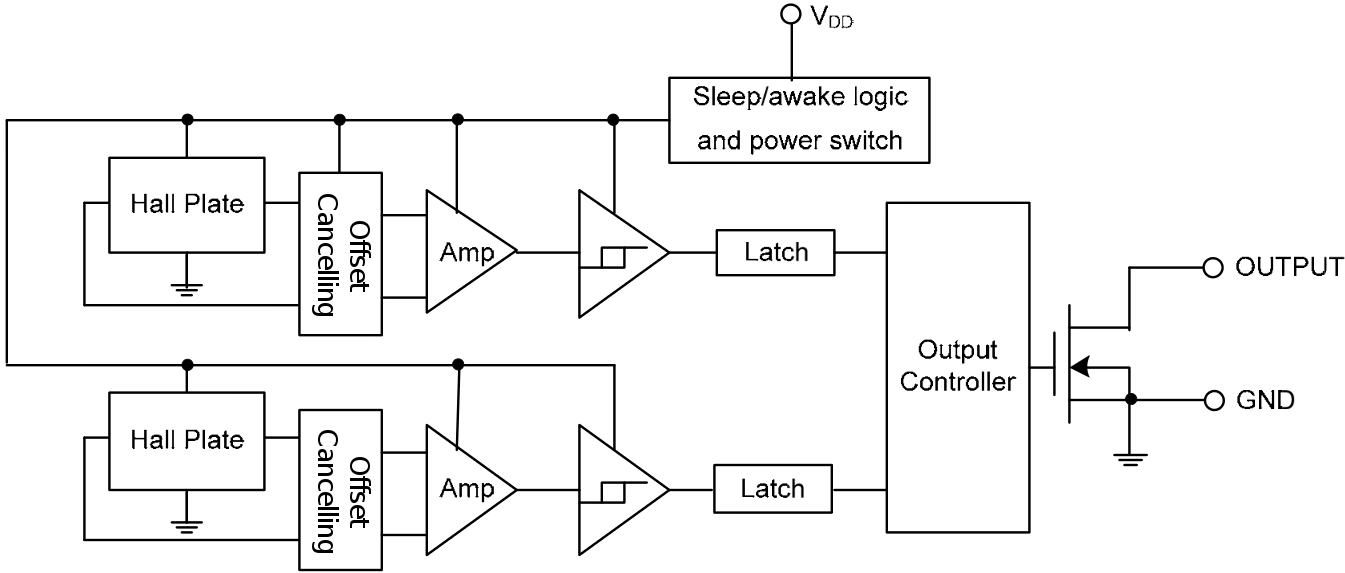
\includegraphics[width=0.75\textwidth]{\EtPath/Bilder/AH180N_functional.png}
	\caption{Funktionelles Blockschaltbild des Hall-Effekt-Schalters AH180N}
	\label{fig:AH180N_functional}
\end{figure}
\fi
%
\ifEMBED
\begin{figure}[h!]
	\centering
	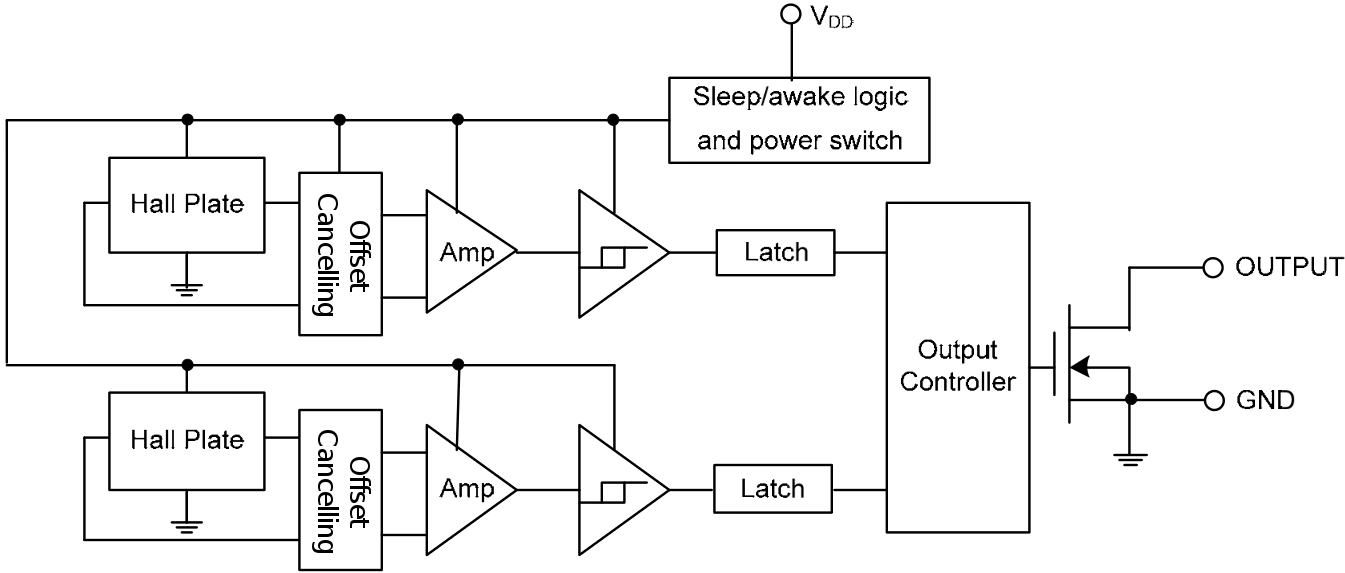
\includegraphics[width=0.75\textwidth]{\EtPath/Bilder/AH180N_functional.png}
	\caption{Funktionelles Blockschaltbild des Hall-Effekt-Schalters AH180N}
	\label{fig:AH180N_functional}
\end{figure}
\fi
%
Ein solches Verfahren lohnt sich bei schnellen Winkelgeschwindigkeiten
und ist für diesen Anwendungsfall sehr effizient. Zugehörige
Hall-Effekt-Schalter lassen sich einfach montieren und sind gegen Störungen
sehr robust. Ein mögliches Modell für einen Hall-Effekt-Schalter ist der
AH180N. Dieser bietet einen Open-Drain Ausgang, welcher somit logische Pegel
liefert (siehe Abbildung \ref{fig:AH180N_functional}). Interessant ist diese
Art von Drehzahl-Geber insbesondere durch ihren geringen Preis, denn solche
Hall-Effekt-Schalter, wie der AH180N, befinden sich im Preissegment von 
unter einem Franken.
    \clearpage
\fi

\ifSTEPPER
    \renewcommand{\EtPath}{src/stepper}
    \ifSTANDALONE
    \section{Schrittmotor} \label{sec:stepper}
\fi
\ifEMBED
    \subsection{Schrittmotor} \label{sec:stepper}
\fi
\ifEMBED
    % Dieses Kapitel ist eine Zusammenarbeit der Gruppen \BLDCTeams. 
    \BLDCcollab
\fi
    Schrittmotoren oder auch Stepper genannt, sind Synchronmotoren, bei 
    welchen der Rotor um einen bestimmten Winkel gedreht werden kann. So ist 
    die Rotorposition ohne zusätzliche Sensoren bekannt. Dabei ist zu 
    beachten, dass der Motor keine Schritte verliert, was bei Überlast 
    geschehen kann. Da die meisten Schrittmotorensysteme Open- Loop Systeme 
    sind, entsteht eine dauernde Positionsabweichung bei einem Schrittverlust. 
    Grundsätzlich wird zwischen zwei Schrittmotortypen unterschieden: 
    \begin{itemize}
       	\item Permanentmagnetmotor
       	\item Reluktanzmotor
    \end{itemize} 
    Der Permanentmagnetmotor besitzt als Rotor einen Permanentmagneten. Beim 
    Reluktanzmotor besteht der Rotor aus einem gezahnten Weicheisenkern. 
    Permanentmagnetmotoren erreichen eine kleinere Schrittfrequenz, besitzen 
    jedoch ein grösseres Drehmoment als Reluktanzmotoren. Die Kombination 
    aus Reluktanzmotor und Permanentmagnetmotor ist ein Hybridmotor. Ein 
    Hybridmotor verbindet die Vorteile von Reluktanz- und Permanentmotor. 

\ifSTANDALONE
    \subsection{Schritte} \label{sec:steps}
\fi
\ifEMBED
    \subsubsection{Schritte} \label{sec:steps}
\fi
    Der Vollschrittbetrieb kann ein- oder auch zweiphasig gesteuert 
    werden. Beim einphasigen Vollschrittbetrieb sind immer zwei gegenüber 
    liegende Pole aktiv. Beim zweiphasigen Vollschrittbetrieb werden jeweils 
    zwei nebeneinander liegende Pole aktiv. Im Halbschrittbetrieb werden die 
    beiden Vollschrittbetriebsarten kombiniert. So kann der Schrittwinkel 
    halbiert werden. Zusätzlich kann der Schrittmotor mit Mikroschritten 
    betrieben werden. Dabei folgt der Strom der sinusförmigen 
    Referenzspannung. (Vgl. Seite \pageref{stromgesteuert}) 
    \begin{figure}[h!]
    	\centering
    	\begin{tikzpicture}
        % Hilfslinien
        \foreach \i in {0, 0.5, ..., 4.5}
        {
            \draw[ultra thin, gray] (\i, 1.9) -- (\i, -0.7);
        }
        % Achsen
    	\draw[->]	(0, 0) -- (0, 2);
    	\draw[->]	(0, 1.2) -- (5, 1.2) node[right]{A};
    	\draw[->]	(0, 0) -- (5, 0) node[right]{B};
        % Kurven
        \draw[red] 
            (0     ,0.7) --
            (0.5   ,0.7) --
            (0.5   ,1.2) --
            (1     ,1.2) --
            (1     ,1.7) --
            (1.5   ,1.7) --
            (1.5   ,1.2) --
            (2     ,1.2) --
            (2     ,0.7) --
            (2.5   ,0.7) --
            (2.5   ,1.2) --
            (3     ,1.2) --
            (3     ,1.7) --
            (3.5   ,1.7) --
            (3.5   ,1.2) --
            (4     ,1.2) --
            (4     ,0.7) --
            (4.5   ,0.7);
        \draw[red] 
            (0      ,0) --
            (0.5    ,0) --
            (0.5    ,0.5) --
            (1      ,0.5) --
            (1      ,0) --
            (1.5    ,0) --
            (1.5    ,-0.5) --
            (2      ,-0.5) --
            (2      ,0) --
            (2.5    ,0) --
            (2.5    ,0.5) --
            (3      ,0.5) --
            (3      ,0) --
            (3.5    ,0) --
            (3.5    ,-0.5) --
            (4      ,-0.5) --
            (4      ,0) --
            (4.5    ,0) ;
    	\end{tikzpicture}
    	\caption{Vollschritt}
    	\label{fig:vollschritt}
    \end{figure}
    \begin{figure}[h!]
     	\centering
     	\begin{tikzpicture}
        % Hilfslinien
        \foreach \i in {0, 0.25, ..., 4.5}
        {
            \draw[ultra thin, gray] (\i, 1.9) -- (\i, -0.7);
        }
        % Achsen
    	\draw[->]	(0, 0) -- (0, 2);
    	\draw[->]	(0, 1.2) -- (5, 1.2) node[right]{A};
    	\draw[->]	(0, 0) -- (5, 0) node[right]{B};
        % Kurven
        \draw[red] 
            (0     ,0.7) --
            (0.75   ,0.7) --
            (0.75   ,1.2) --
            (1     ,1.2) --
            (1     ,1.7) --
            (1.75   ,1.7) --
            (1.75   ,1.2) --
            (2     ,1.2) --
            (2     ,0.7) --
            (2.75   ,0.7) --
            (2.75   ,1.2) --
            (3     ,1.2) --
            (3     ,1.7) --
            (3.75   ,1.7) --
            (3.75   ,1.2) --
            (4     ,1.2) --
            (4     ,0.7) --
            (4.5   ,0.7);
        \draw[red] 
            (0      ,-0.5) --
            (0.25   ,-0.5) --
            (0.25   ,0) --
            (0.5    ,0) --
            (0.5    ,0.5) --
            (1.25   ,0.5) --
            (1.25   ,0) --
            (1.5    ,0) --
            (1.5    ,-0.5) --
            (2.25   ,-0.5) --
            (2.25   ,0) --
            (2.5    ,0) --
            (2.5    ,0.5) --
            (3.25   ,0.5) --
            (3.25   ,0) --
            (3.5    ,0) --
            (3.5    ,-0.5) --
            (4.25   ,-0.5) --
            (4.25   ,0) --
            (4.5    ,0) ;
     	\end{tikzpicture}
     	\caption{Halbschritt}
     	\label{fig:halbschritt}
    \end{figure}
    \begin{figure}[h!]
    	\centering
    	\begin{tikzpicture}
        % Hilfslinien
        \foreach \i in {0, 0.05, ..., 4.5}
        {
            \draw[ultra thin, gray] (\i, 1.9) -- (\i, -0.7);
        }
        % Achsen
    	\draw[->]	(0, 0) -- (0, 2);
    	\draw[->]	(0, 1.2) -- (5, 1.2) node[right]{A};
    	\draw[->]	(0, 0) -- (5, 0) node[right]{B};
        % Kurven
        \foreach \i in {0, 0.05, ..., 4.5}
        {
            \draw[red] (\i, {0.5*sin(180*\i)})          -- (\i+0.05, {0.5*sin(180*\i)});
            \draw[red] (\i, {0.5*sin(180*\i+(90))+1.2}) -- (\i+0.05, {0.5*sin(180*\i+(90))+1.2});
        }
    	\end{tikzpicture}
    	\caption{Mikroschritt}
    	\label{fig:mikroschritt}
    \end{figure}

    \noindent
    Wie bei anderen Motoren hat auch bei Schrittmotoren die Anzahl Polpaare 
    einen Einfluss auf dessen Drehzahl. Die Polpaare bilden eine Untersetzung 
    zwischen der elektrischen und der mechanischen Rotation. Die meisten 
    gängigen Schrittmotoren besitzen 50 Polpaare. Da eine elektrische 
    Umdrehung aus vier Schritten besteht ergeben sich bei 50 Polpaaren 200 
    Schritte für eine Umdrehung. Dies ergibt eine Schrittauflösung von 
    1.8\si{\degree} bei Vollschrittbetrieb. 

\ifSTANDALONE
    \subsection{Wicklungen} \label{sec:windings}
\fi
\ifEMBED
    \subsubsection{Wicklungen} \label{sec:windings}
\fi
    Ein Schrittmotor besitzt zwei getrennte Wicklungen. Diese sind 
    rechtwinklig zueinander angeordnet. Bei Motoren mit mehr als einem Polpaar 
    sind entsprechend mehr Wicklungen verbaut. Beim Aufbau der Wicklungen 
    wird zwischen unipolaren und bipolaren Wicklungen unterschieden. 
    %
    Die unipolare Wicklung besitzt einen Mittelabgriff. Dieser wird meistens 
    mit der Versorgungsspannung verbunden. Die beiden anderen Enden werden nun 
    mit einer Lowside Treiberstufe angesteuert. Dadurch kann der magnetische 
    Fluss mit einem geringen elektronischen Aufwand umgekehrt werden. Jedoch 
    ist immer nur eine Hälfte der Wicklung aktiv. Zudem ist die Herstellung 
    aufwendiger und somit auch teurer. 
    %
    Bei einer bipolaren Wicklung fehlt der mittlere Abgriff. Die Umkehrung des 
    magnetischen Flusses muss über die Umkehrung der angelegten Spannung 
    erfolgen. Deshalb muss für beide Wicklungen jeweils eine Brückenschaltung 
    verwendet werden. Da bei bipolaren Schrittmotoren immer die gesamte 
    Wicklung verwendet wird, kann damit ein grösseres Drehmoment erzeugt 
    werden als mit einem gleich grossen unipolaren Schrittmotor. 
    %
    Die Ansteuerung der beiden Wicklungsarten ist in \autoref{fig:uniVsbi} 
    ersichtlich. \cite{Doku:Stepper}
    \begin{figure}[h!]
       	\centering
       	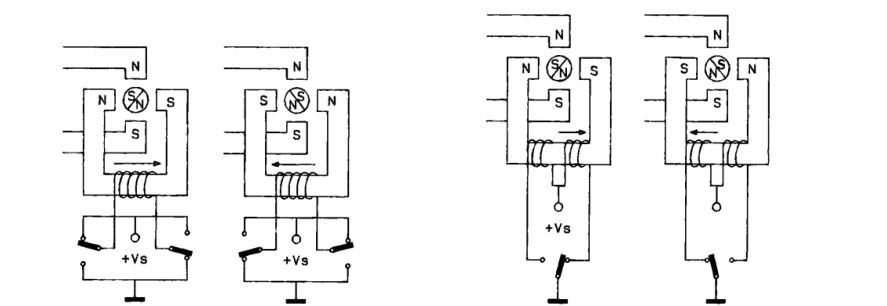
\includegraphics[width=12cm]{\EtPath/Bilder/uniVsbi.jpg}
       	\caption[Bipolarer und unipolarer Betrieb]{bipolarer und unipolarer Betrieb \cite{Doku:Stepper}}
       	\label{fig:uniVsbi}
    \end{figure}
    
       
    

    \clearpage
    \ifSTANDALONE
\section{Stepper Motoransteuerung}
\fi
\ifEMBED
\subsection{Stepper Motoransteuerung}
\fi

\ifEMBED
    % Dieses Kapitel ist eine Zusammenarbeit der Gruppen \BLDCTeams. 
    \BLDCcollab
\fi
\ifSTANDALONE
    \subsection{Grundsätzliches zur Ansteuerung}\label{subsec:Ansteuerung}
\fi
\ifEMBED
    \subsubsection{Grundsätzliches zur Ansteuerung}\label{subsec:Ansteuerung}
\fi
	Grundsätzlich besteht die Ansteuerung aus drei Teilen, wie in 
    \autoref*{fig:ansteuerung} gezeigt. 
    Um die Ansteuerung zu realisieren, gibt es eine Vielzahl von 
    integrierten Schaltkreisen. Diese unterscheiden sich wie folgt: 
    \begin{itemize}
    	\item \textbf{Interfaces:} Einzelanschlüsse, einfache 
            Busschnittstellen oder Mikrocontrollerschnittstellen wie SPI, 
            II2
    	\item \textbf{Steuerfunktionen:} Einzelne Schritte oder 
            Bewegungsabläufe (Motion Control Function)
    	\item \textbf{Schaltungsintegration:} Steuerung und Treiberstufe als 
            getrennte Schaltkreise, oder in einem Schaltkreis zusammengefasst. 
        \item[] \cite{Doku:Stepper} 
    \end{itemize}
    
    \noindent
    Der gewählte integrierte Schaltkreis ist der L6480 von 
    STMicroelectronics. Dieser wird über die SPI Schnittstelle gesteuert 
    und besitzt eine Motion Contol Engine. Die Treiberstufe wird extern 
    realisiert. (Vgl. Kapitel \ref{sec:L6480}) 
	\begin{figure}[h!]
		\centering
		\begin{tikzpicture}
		\draw[line width=1.5pt](0, 0) rectangle node{Mikrocontroller} (3, 1)  ;
		\draw[line width=1.5pt, ->]	(3, 0.5) -- (4, 0.5);
		\draw[line width=1.5pt](4, 0) rectangle node{Steuerung}(7, 1);
		\draw[line width=1.5pt, ->]	(7, 0.5) -- (8, 0.5);
		\draw[line width=1.5pt](8, 0) rectangle node{Treibertufen}(11, 1);
		\end{tikzpicture}
		\caption{Komponenten der Ansteuerung eines Schrittmotores}
		\label{fig:ansteuerung}
	\end{figure}
    
\ifSTANDALONE
\subsection{Treiberstufe}
\fi
\ifEMBED
\subsubsection{Treiberstufe}
\fi 
	Wird ein Schrittmotor unipolar betrieben, so können die vier Wicklungen 
    direkt mit Lowside Treibern angesteuert werden. Für den bipolaren 
    Betrieb benötigt man für beide Wicklungen je eine H-Brücke. Die 
    einfachste Methode ist es, den Strom nur durch den Wicklungswiderstand 
    zu begrenzen. Der Nachteil ist, dass die Zeitkonstante durch den 
    Wicklungswiderstand und die Induktivität bestimmt ist, und so bei 
    höheren Schrittfrequenzen der gewünschte Strom und damit das 
    Drehmoment nicht mehr erreicht wird. Deshalb wird ein zusätzlicher 
    Vorwiderstand in Serie geschaltet, und so die Zeitkonstante 
    verkleinert. Typische Verhältnisse sind vierfacher- oder fünffacher 
    Widerstand, was eine vierfache bzw. fünffache Speisespannung 
    voraussetzt. Diese Methode wiederum führt zu einer höheren 
    Verlustleistung in den Widerständen. Im Ruhezustand ist es sinnvoll, 
    den Strom soweit zu senken, dass das Haltemoment nicht unterschritten 
    wird. Eine Spannungsumschaltung hat den weiteren Vorteil, dass so beim 
    Anfahren eine steilere Stromkurve erreicht werden kann. (Vgl. 
    \autoref{fig:spannungsumschaltung})
	 \begin{figure}[h!]
	 	\centering
	 	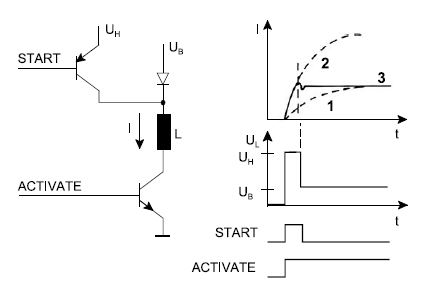
\includegraphics[width=8cm]{\EtPath/Bilder/spannungsumschaltung.jpg}
	 	\caption[Spannungsumschaltung]{Spannungsumschaltung \cite{AppNote:Stepper}}
	 	\label{fig:spannungsumschaltung}
	 \end{figure}

    \noindent
	Der Schrittmotor kann alternativ auch stromgesteuert betrieben werden. 
    Dabei folgt der Stromverlauf dem Verlauf einer Referenzspannung 
    (Sollwert). Der Stromverlauf wird auf den Sollwert geregelt. Die 
    Betriebsspannung muss so nicht stabilisiert werden. 
    \label{stromgesteuert} 


    \clearpage
    \ifSTANDALONE
    \section{Stepper Driver L6480} \label{sec:L6480}
\fi
\ifEMBED
    \subsection{Stepper Driver L6480} \label{sec:L6480}
\fi
\ifEMBED
    % Dieses Kapitel ist eine Zusammenarbeit der Gruppen \BLDCTeams. 
    \BLDCcollab
\fi
Wie bereits im Kapitel \ref*{subsec:Ansteuerung} erwähnt, wird der L6480 von STMicroelectronics verwendet. 

\ifSTANDALONE
    \subsection{Funktionsbeschreibung}
\fi
\ifEMBED
    \subsubsection{Funktionsbeschreibung}
\fi
    Diese Schrittmotorensteuerung ist für den Betrieb von zweiphasigen (Vgl. 
    Kpaitel \ref{sec:stepper}) Schrittmotoren mit Mikrosteps (Vgl. Kapitel 
    \ref{sec:stepper}) geeignet. Der L6480 erreicht eine maximale Auflösung 
    von einem 1/128 Schritt. Die Steuerung generiert intern die PWM- Signale 
    für die Motorenansteuerung. Alternativ kann auch mit Vollschritten oder 
    Halbschritten gearbeitet werden. Die beiden H- Brücken werden extern mit 
    N-Kanal MOSFETs realisiert. Es können Bewegungsprofile konfiguriert 
    werden, so dass die Motoren definiert anfahren, abbremsen oder ein Punkt 
    direkt angefahren werden kann. So kann der Aufwand bei der 
    Mikrocontrollerprogrammierung verringert werden. Die Befehle werden über 
    eine SPI- Schnittstelle übertragen. Die absolute Position ist in einem 22- 
    Bit Register gespeichert. Der Bereich liegt dementsprechend zwischen 
    \(-2^{21}\) und \(2^{21}-1\). \cite{Datasheet:L6480} 

\ifSTANDALONE
    \subsection{Schnitstelle}
\fi
\ifEMBED
    \subsubsection{Schnittstelle}
\fi
Der steuernde Mikrocontroller benötigt 8 Pins für die Kommunikation mit dem 
L6480 \cite{Datasheet:L6480} : 
\begin{table}[h!]
    \begin{zebralongtable}{l l p{7cm}}
        \rowcolor{gray}\textbf{Pin} &
            \textbf{IO} &
            \textbf{Funktion} \\
        $\overline{FLAG}$ &
            Output (Open Drain) &
            Wird bei einem Fehler intern auf GND gezogen. \\
        $\overline{BUSY}$ / SYNC &
            Output (Open Drain) &
            Wird während dem Ausführen eines Befehls intern auf GND gezogen.\\
        $\overline{STBY / RESET}$ &
            Input &
            Standby- und Resetmodus, falls extern GND anliegt. \\
        STCK &
            Input &
            Im Step-Clock- Mode führt jede positive Flanke an diesem Pin zu einem 
                Schritt. \\
        \rowcolor{gray}\textbf{SPI} & & \\
        $\overline{CS}$ &
            Input &
            Chip Select: Falls extern GND anliegt, startet die Kommunikation. Um 
                die Kommunikation zu beenden, muss $\overline{CS}$ extern auf High 
                gehalten werden. \\
        CK &
            Input &
            Serial Clock: Synchronisierung der Kommunikation. \\
        SDO &
            Output &
            Slave Data Out: Daten für den Mikrocontroller. \\
        SDI &
            Input &
            Slave Data In: Befehle und Daten für den L6480. \\
    \end{zebralongtable}
    \caption{Schnittstelle des Treibers L6480}
    \label{tab:Schnittstelle}
\end{table}
%\begin{longtable}{l l p{7cm}} \toprule
%    \textbf{Pin}    & \textbf{IO}   & \textbf{Funktion} \\
%    \midrule
%    \endhead
%    \multicolumn{3}{l}{\emph{Fortsetzung auf nächster Seite}} \\ \bottomrule \endfoot \endlastfoot          
%    \textbf{IO}\\ \addlinespace
%    %\cmidrule{1-1}
%    $\overline{FLAG}$& Output               & Wird bei einem Fehler intern auf GND gezogen. \\ \addlinespace
%    $\overline{BUSY}$ / SYNC & Output       & Wird während dem Ausführen eines Befehls intern auf GND gezogen.\\ \addlinespace
%    $\overline{STBY / RESET}$& Input        & Standby- und Resetmodus, falls extern GND anliegt. \\ \addlinespace
%    STCK            & Input         & Im Step-Clock- Mode führt jede positive Flanke an diesem Pin zu einem Schritt. \\ \addlinespace
%    %\cmidrule{1-1}
%    \textbf{SPI}\\ \addlinespace
%    %\cmidrule{1-1}
%    $\overline{CS}$ & Input         & Chip Select: Falls extern GND anliegt, startet die Kommunikation. Um die Kommunikation zu beenden, muss $\overline{CS}$ extern auf High gehalten werden. \\ \addlinespace
%    CK              & Input         & Serial Clock: Synchronisierung der Kommunikation. \\ \addlinespace
%    SDO             & Output        & Slave Data Out: Daten für den Mikrocontroller. \\ \addlinespace
%    SDI             & Input         & Slave Data In: Befehle und Daten für den L6480. \\ \addlinespace
%    \bottomrule
%    \\
%    \caption{Schnittstelle} 
%    \label{tab:Schnittstelle}
%\end{longtable} 

\ifSTANDALONE  
    \newpage 
    \subsection{Typical Application}
\fi
\ifEMBED
    \subsubsection{Typical Application}
\fi
\begin{figure}[h]
    \centering
    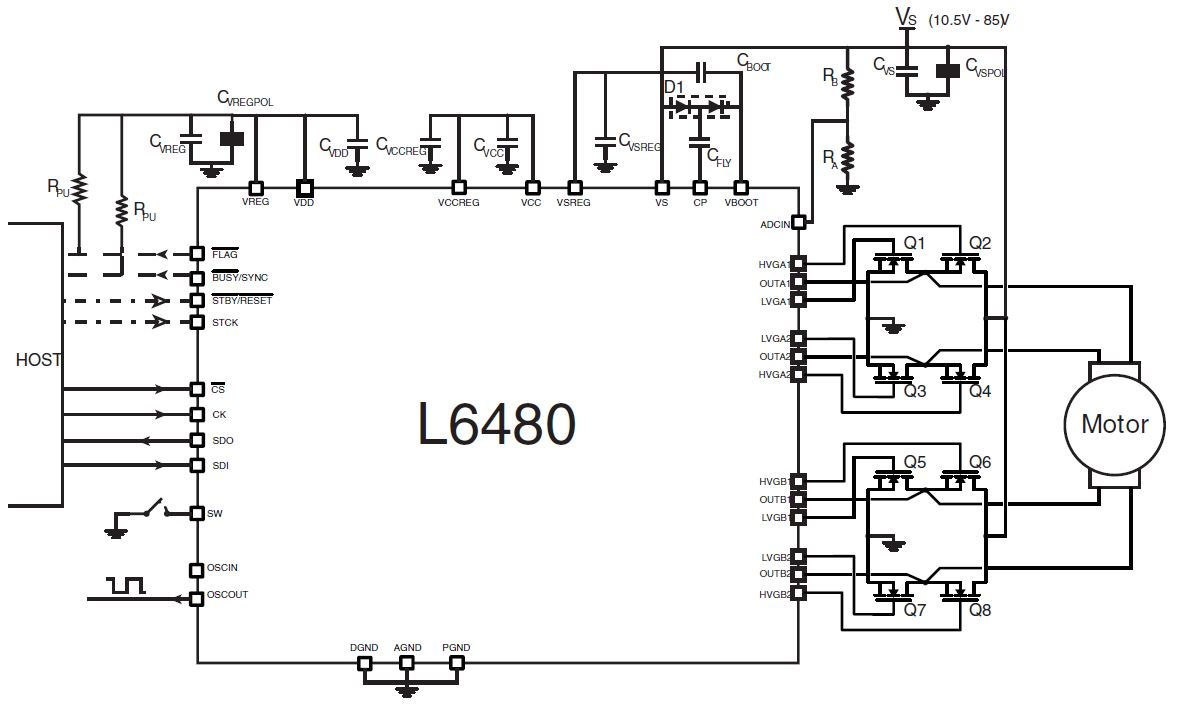
\includegraphics[width=12cm]{\EtPath/Bilder/typicalApp.jpg}
    \caption[Typical Application]{Typical Application \cite{Datasheet:L6480}}
    \label{fig:typApp}
\end{figure}

    \clearpage
    \ifSTANDALONE
\section{Realisierung}
\fi
\ifEMBED
\subsection{Realisierung}
\fi 
    \ifSTANDALONE
    \subsection{Hardware} \label{ch:Hardware}
    \fi
    \ifEMBED
    \subsubsection{Hardware} \label{ch:Hardware}
    \fi
    Der L6480 besitzt, wie in \autoref{sec:L6480} beschrieben, eine 
    SPI-Schnittstelle. Über diese Schnittstelle soll der Steppertreiber die 
    Befehle des Freedomboards erhalten. Der Steppertreiberprint wird mit 
    Stiftleisten bestückt und kann so direkt auf das Freedomboard aufgesteckt 
    werden. Es wird so keine Kabelverbindung benötigt und die Elektronik 
    bleibt kompakt.
    \begin{figure}[h]
        \centering
        \begin{tikzpicture}
        \node[above right] (img) at (0,0) {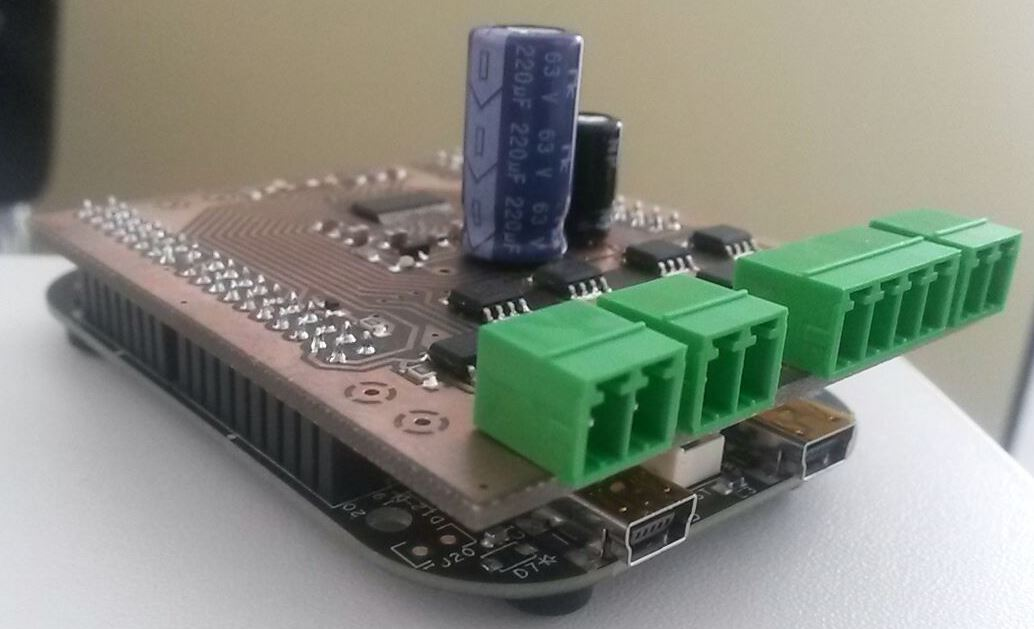
\includegraphics[width=8cm]{\EtPath/Bilder/hardware.jpg}};
        \draw[line width=1pt]
        (1.5, 0.75) node[below=1mm] {Freedom-Board}
        -- (2.7, 1);
        \fill (2.7,1) circle (2pt);
        \draw[line width=1pt]
        (2, 4) node[above=2mm] {Adapterprint}
        -- (2.7, 2);
        \fill (2.7,2) circle (2pt);
        \end{tikzpicture}
        \caption{Freedomboard und Steppertreiberprint}
        \label{fig:Steppertreiber}
    \end{figure}
    \newline
    Der Steppertreiberprint beinhaltet grundsätzlich den Treiber für den 
    Schrittmotor, realisiert mit dem Baustein L6480 und einer externen 
    H-Brücke aus N-FET. Zusätzlich sind Anschlüsse für andere Motoren (z.B.  
    BLDC-Motor) auf dem Print integiert. Im Folgenden wird die Entwicklung 
    dieses Adapterprints vogestellt. Ab Seite \pageref{sec:Schema} ist das 
    Schema der Schaltung und ab Seite \pageref{sec:PrintDesign} die 
    Beschreibung des Printdesigns zu finden. 
    % -----------------------------------------------------------------------------------
    \ifSTANDALONE
    \subsection{Schema} \label{sec:Schema}
    \fi
    \ifEMBED
    \subsubsection{Schema} \label{sec:Schema}
    \fi
    Als Motorencontroller wird der integrierte Schaltkreis L6480 von 
    STMicroelectronics verwendet. Dieser wird über eine SPI-Schnittstelle 
    angesteuert. Der l6480 bietet die Möglichkeit, Bewegungsprofile zu 
    konfigurieren. Die verschiedenen Betriebsarten werden im Kapitel 
    \ref{ch:Software} vorgestellt. Die H-Brücke wird extern mit N-FETs 
    realisiert. Die Beschaltung des L6480 kann aus dem Datenblatt 
    \cite{Datasheet:L6480} entnommen werden.\\\\ 
    Das revidierte Schema ist auf Seite \pageref{Schema} abgebildet.
    \\\\
    \textbf{Speisung}\\
    Es gibt zwei Möglichkeiten, wie das IC gespiesen werden kann: 
    \begin{itemize}
        \item Motorenspannung, interne Spannungsregler generieren die nötige 
            Gatespannung sowie die Logikspannung
        \item Externe Spannungsregler
    \end{itemize}
    Es wird die erste Möglichkeit, die Speisung mit nur der Motorenspannung 
    gewählt. Als Motorenspeisung ist ein Bereich von 10.5 \ldots 85\si{\volt} 
    zulässig. Bei eine Betriebsspannung von mehre als 25\si{\volt} sind MOSFET 
    mit einer höherenen Sperrspannung notwendig. Zusätzliche Spannungsregler 
    sind nicht notwendig. 
    \\\\
    \textbf{Motor supply voltage compensation}\\
    Der Motorcontoller bietet die Möglichkeit, Schwankungen der 
    Motorenspannung zu erkennen und so die Amplitude des PWM-Sinussignales am 
    Schrittmotor zu regeln. Dazu muss der Eingang ADCIN des Controllers 
    korrekt beschaltet werden. An diesem Analogeingang soll bei korrekter 
    Motorspannung 1/2 der Logikspannung anliegen. In diesem Fall bedeutet 
    dies, dass bei normaler Betriebsspannung 1.65\si{\volt} über dem 
    Widerstand R4 anliegen müssen. 
    \\\\
    \textbf{LED Speisung}\\
    Damit sofort ersichtlich ist, ob der Adapterprint gespiesen ist, wird eine 
    LED vorgesehen. Diese wird zwischen die Speisung über einen Vorwiderstand 
    an GND angeschlossen. Somit ist alles in Ordnung, falls die LED leuchtet.
    \\\\
    \textbf{LED Fehler}\\
    Der Motorencontroller kann so konfiguriert werden, dass verschiedene 
    Fehler angezeigt werden können. Dies beinhaltet zum Beispiel 
    Schrittverluste, Überstrom, Unterspannungserkennung oder Überhitzung des 
    Controllers. Dazu dient ein Open-Drain Pin $\overline{FLAG}$, welcher im 
    Fehlerfall auf GND zieht. Der Pin wird so beschaltet, dass eine LED den 
    Fehlerfall auch optisch sichtbar macht. 
    \\\\
    \textbf{Pinbelegung}\\
    Die Kommunikation mit dem Motorencontroller und die Ansteuerung des 
    Pneumatikventils wird mit dem Freedom-Board realisiert. 
    Die folgende Tabelle stellt die Schnittstelle zwischen dem Freedomboard 
    und den Anschlüssen auf dem Adapterprint dar. 
    \begin{table}[h!]
        \begin{zebralongtable}{p{3cm} p{2cm} p{1.5cm}}
             \rowcolor{gray}\textbf{Pin}                & \textbf{Stepper-board}   & \textbf{FRDM-KL25Z} \\           
            \textbf{IO L6480}\\ 
            %\cmidrule{1-1}
            $\overline{FLAG}$           & J2 Pin 2  & PTA13 \\ 
            $\overline{BUSY}$ / SYNC    & J1 Pin 2  & PTA1  \\ 
            $\overline{STBY / RESET}$   & J2 Pin 11 & PTA17 \\ 
            STCK                        & J2 Pin 9  & PTA16 \\ 
            %\cmidrule{1-1}
            \textbf{SPI L6480}          &           &       \\ 
            %\cmidrule{1-1}
            $\overline{CS}$             & J9 Pin 13 & PTE4  \\ 
            CK                          & J9 Pin 9  & PTE2  \\
            MOSI                        & J9 Pin 11 & PTE3  \\ 
            MISO                        & J2 Pin 20 & PTE1  \\ 
            \textbf{Pneumatik}\\ 
            Ventil                      & J2 Pin 18 & PTE0  \\ 
        \end{zebralongtable}
        \caption{Pinbelegung}
        \label{tab:Pinbelegung}
    \end{table} 
    \\
    \textbf{Zusätzliche Bestückung}\\
    Zusätzlich kann ein Bluetoothmodul bestückt werden. Weitere 
    Bestückungen...\\\\
    Es wird mit dem Tool Altium Designer gearbeitet. Das überarbeitete Schema 
    des Steppertreiberprints ist auf der Seite \pageref{Schema} zu finden. 
    %*****************************************************
    % Schema Stepperboard                                %
    %*****************************************************
    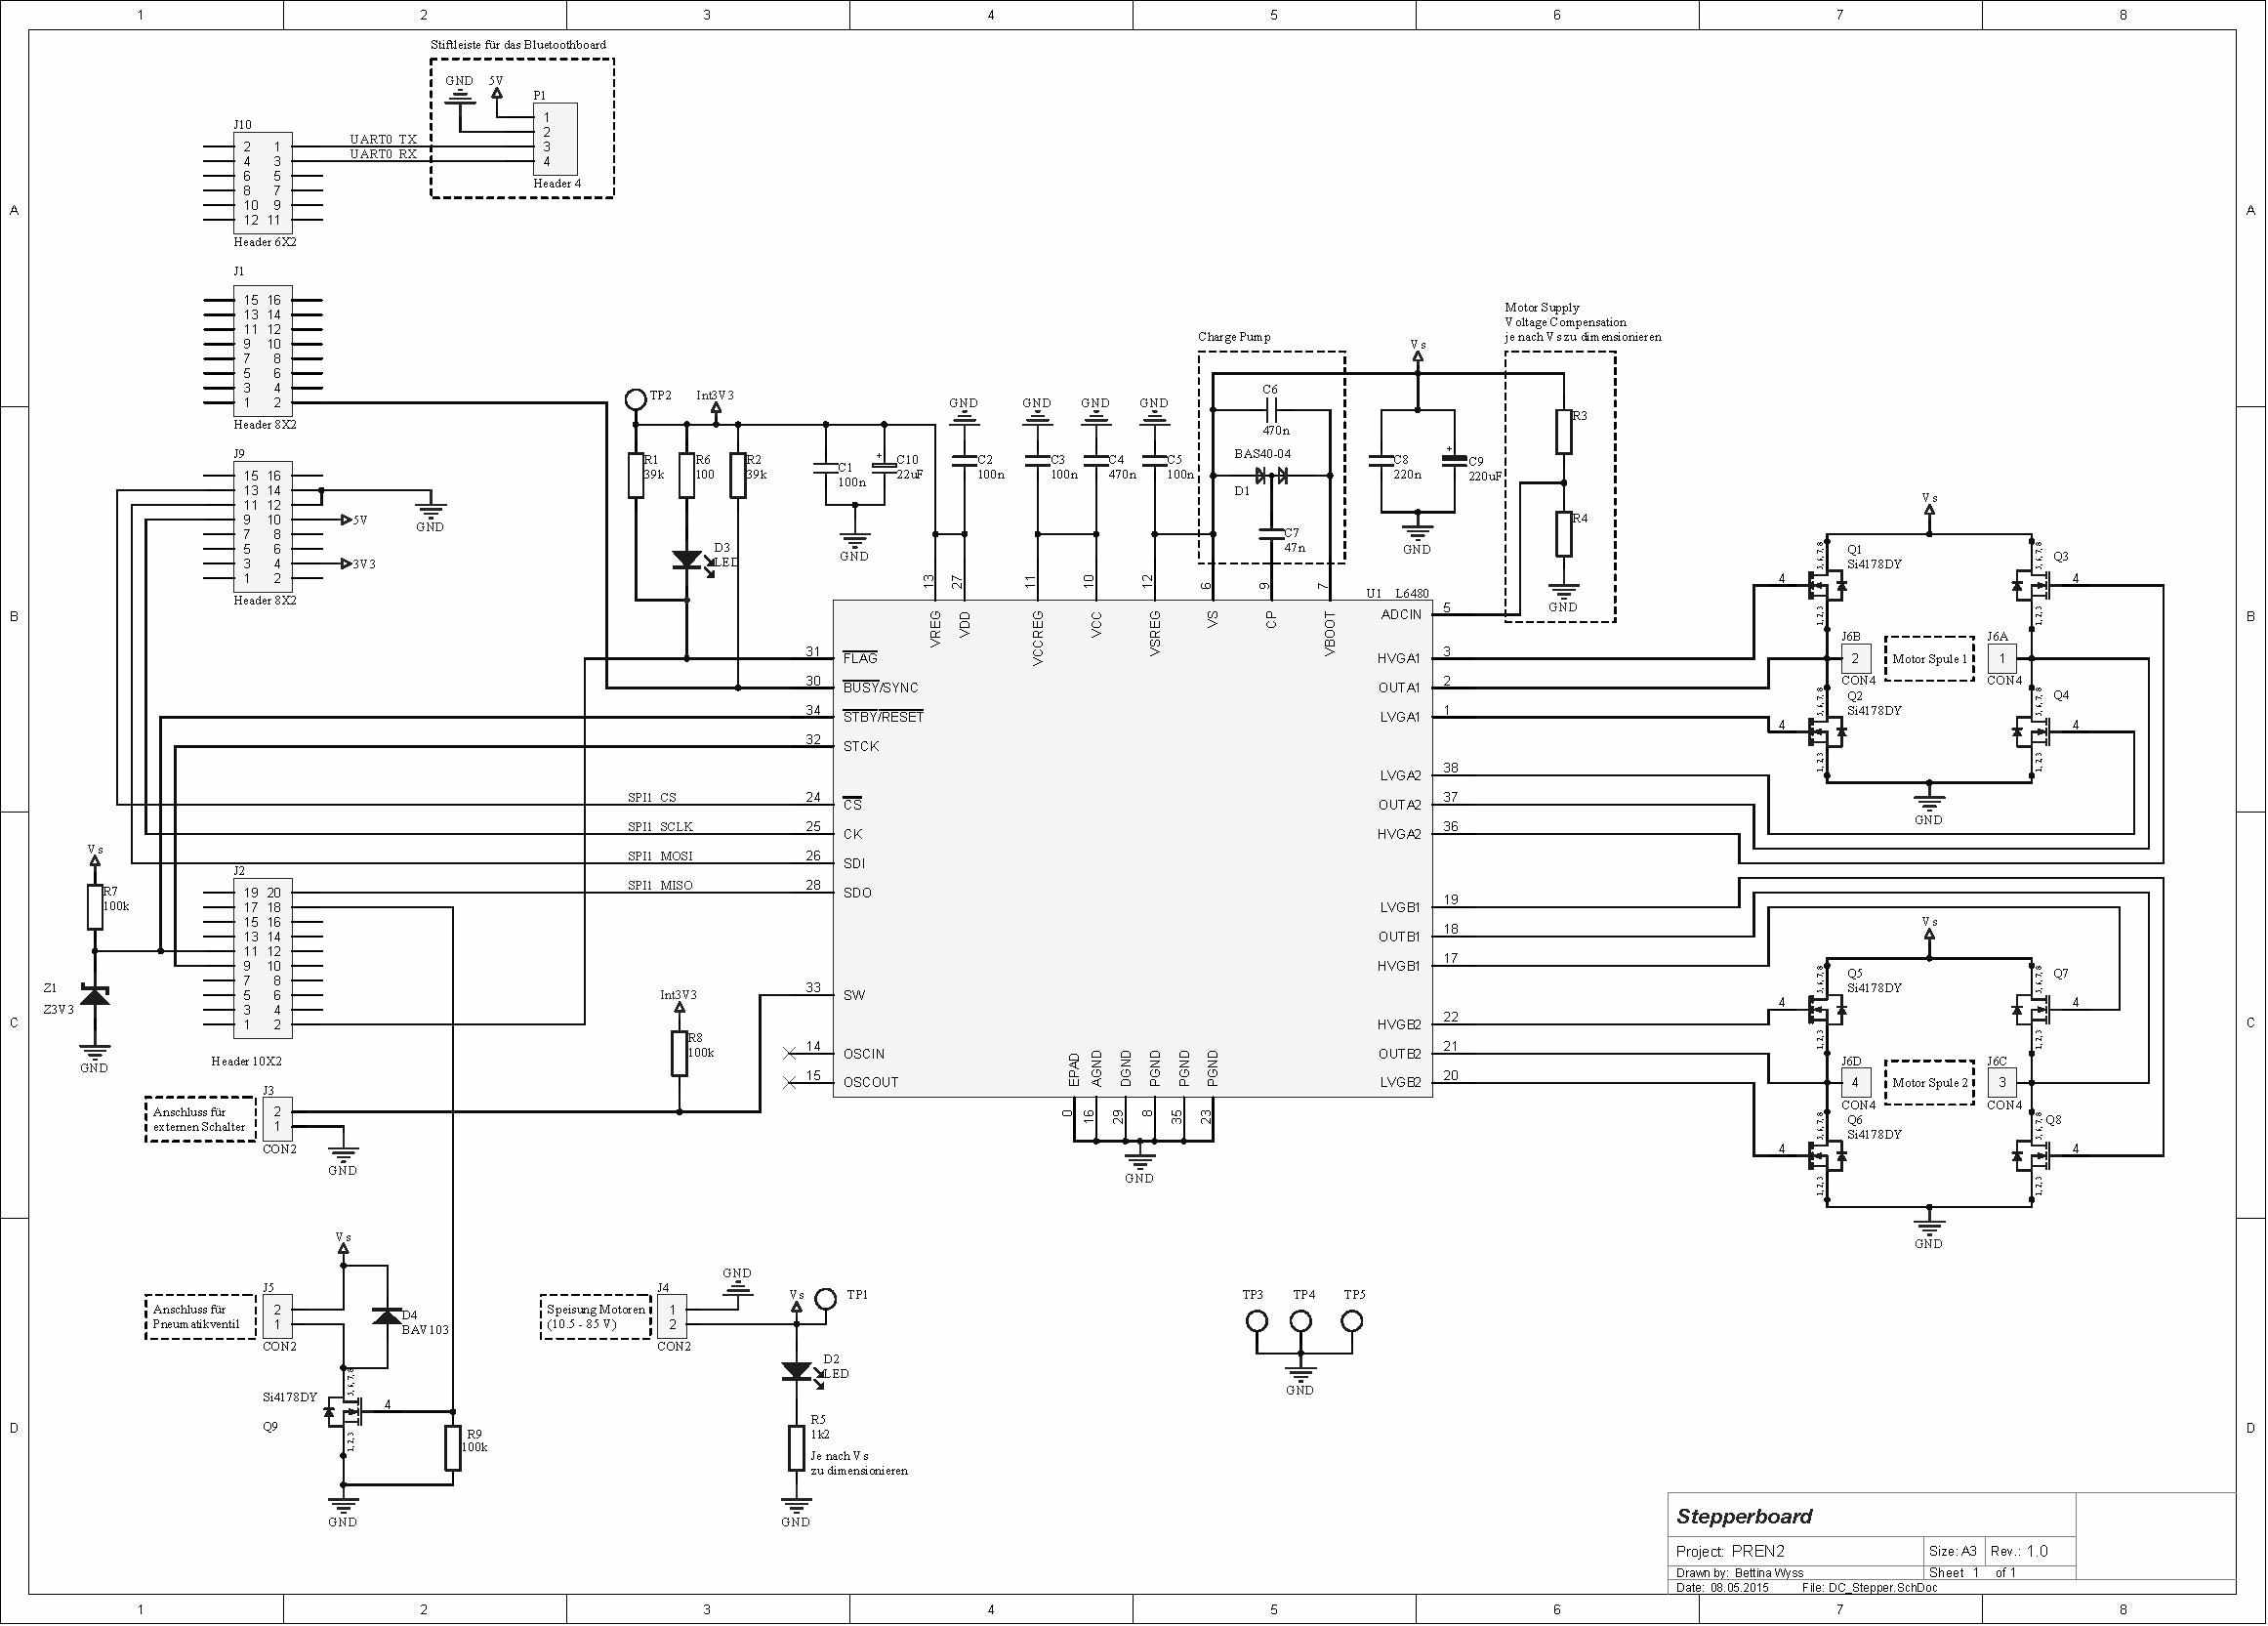
\includepdf[page=1 , offset=0cm -3cm, angle = 90, width=\textwidth,picturecommand={\centering},pagecommand=\subsection*{Schema}\label{Schema}]{\EtPath/Bilder/Stepperboard_Schematic.pdf}
    \newpage
    \subsection*{Bestückungsdokumente}
    \begin{figure}[h!]
        \centering
        \begin{minipage}[hbt]{6cm}
            \centering
            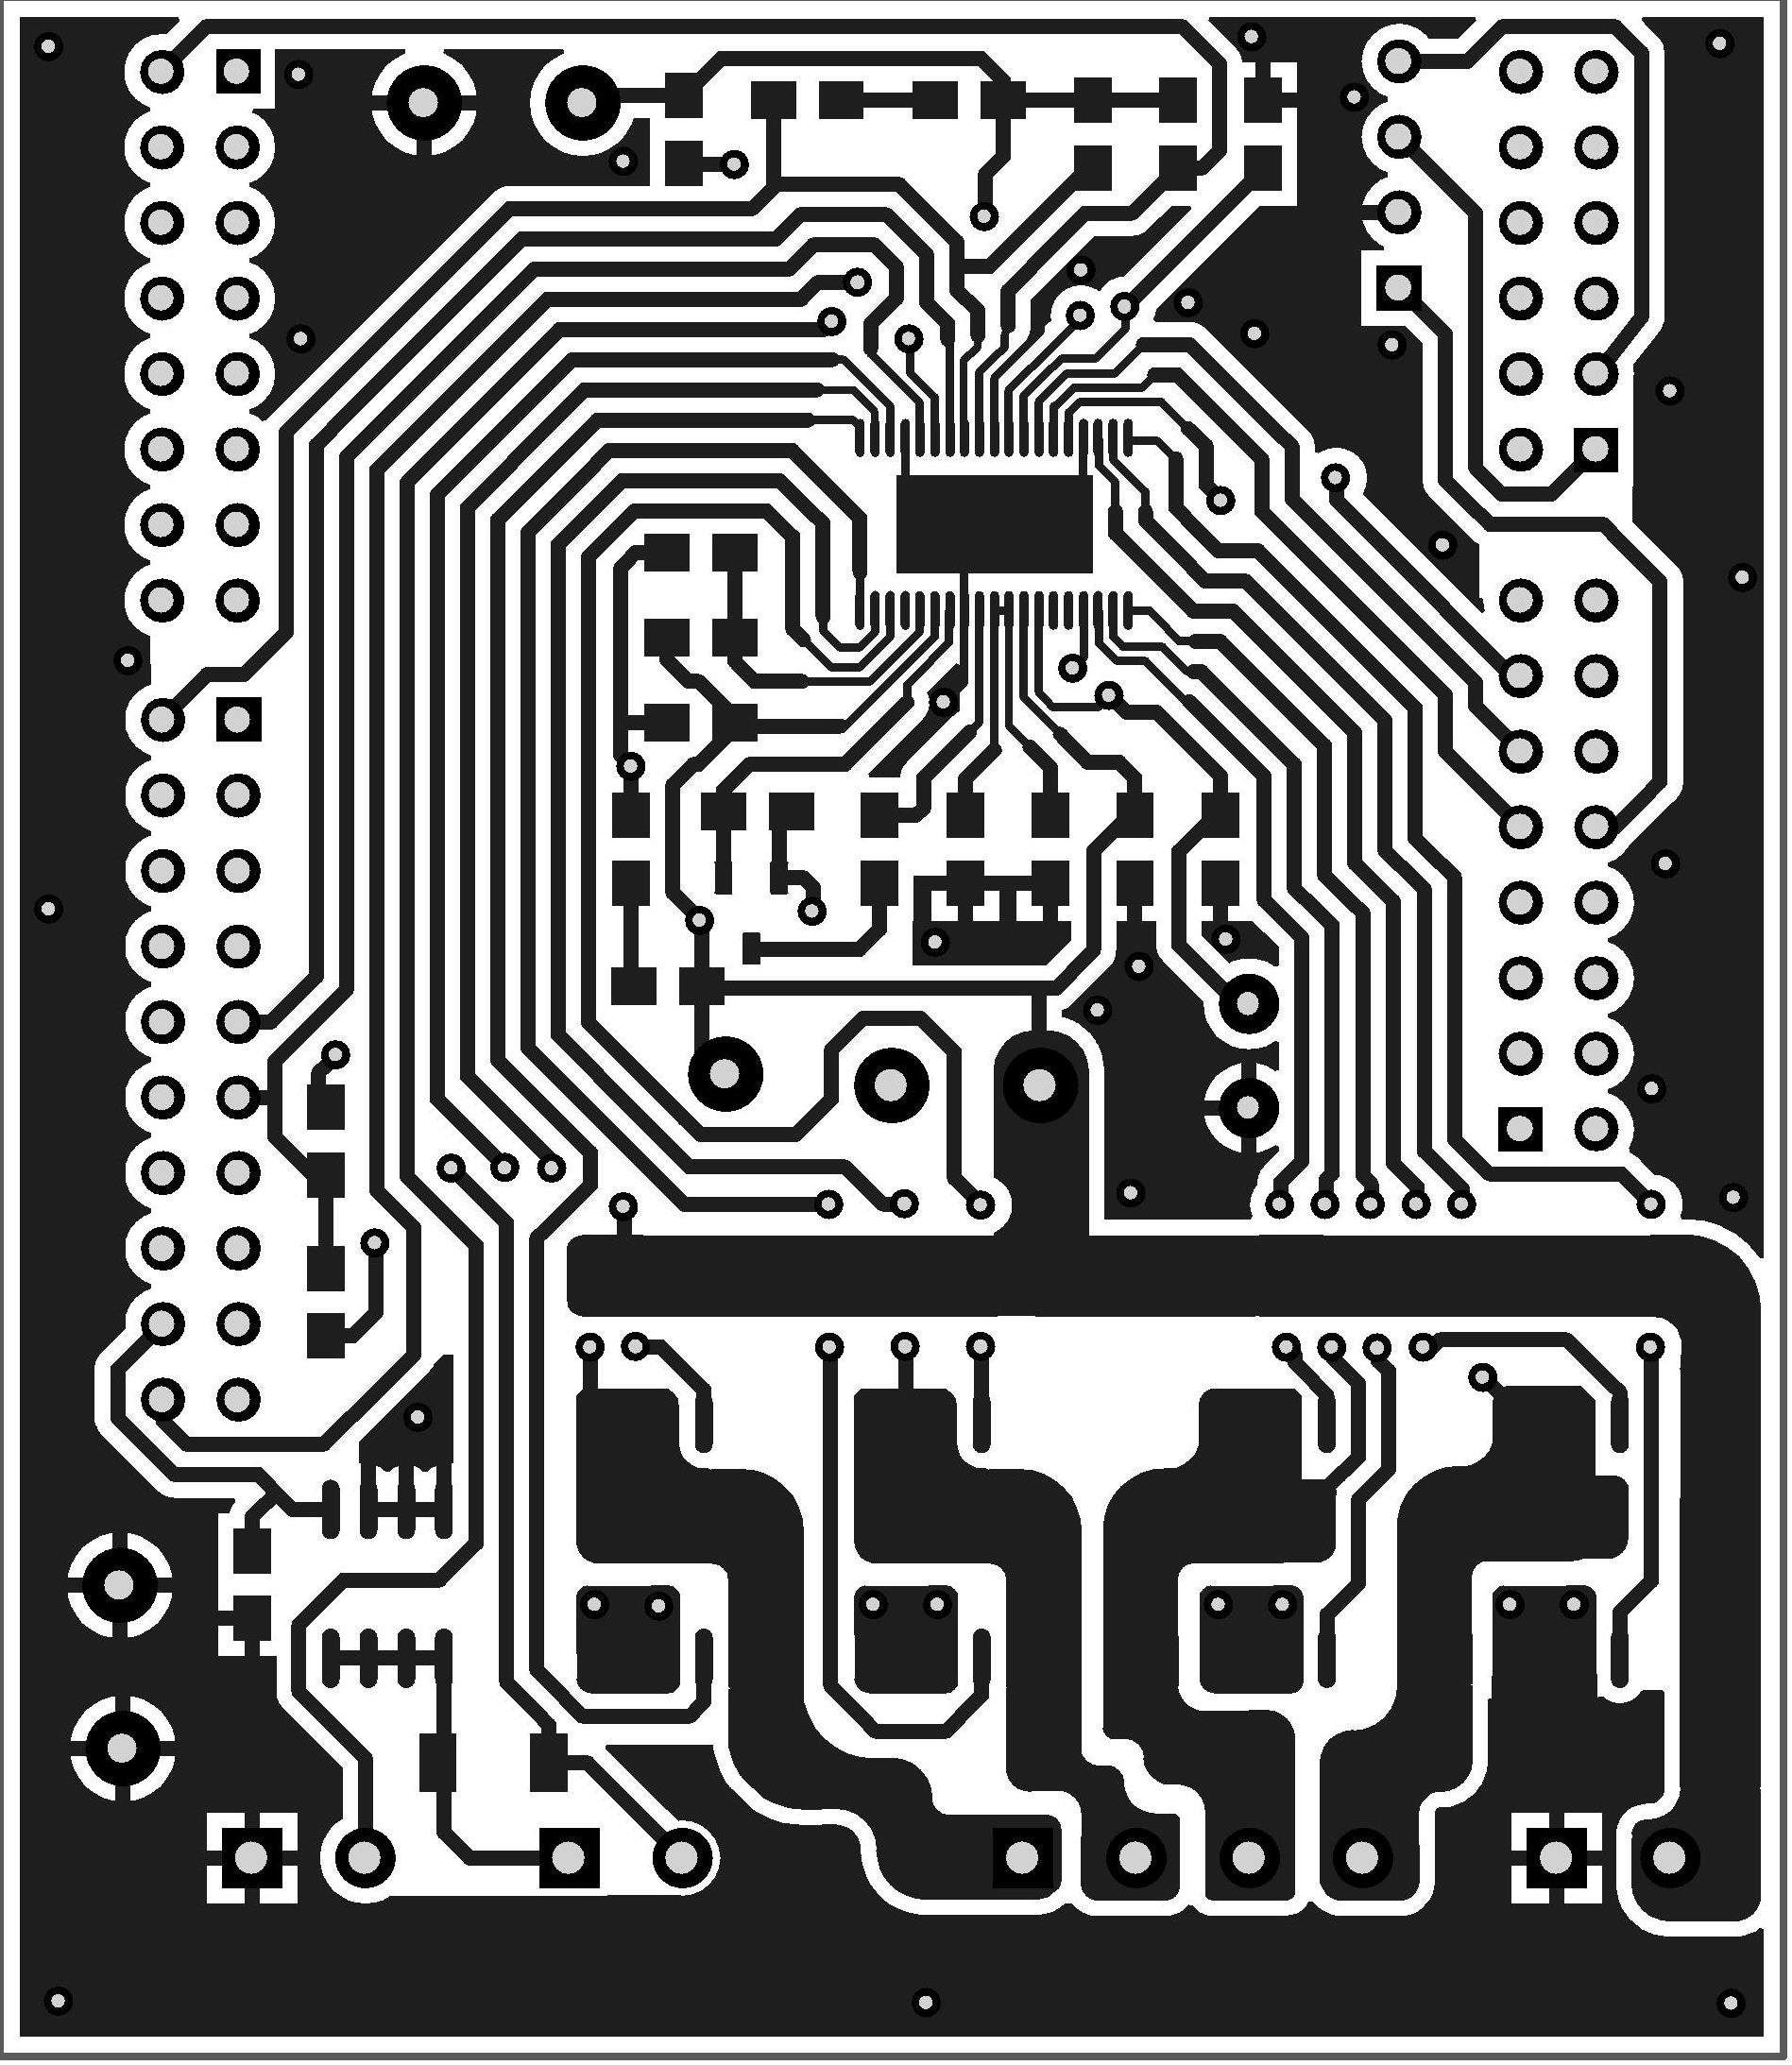
\includegraphics[width=6cm]{\EtPath/Bilder/DC_Stepper0.jpg}
            \caption{Top Layer}
            \label{fig:Top Layer}
        \end{minipage}
        \hspace{1.5cm}
        \begin{minipage}[hbt]{6cm}
            \centering
            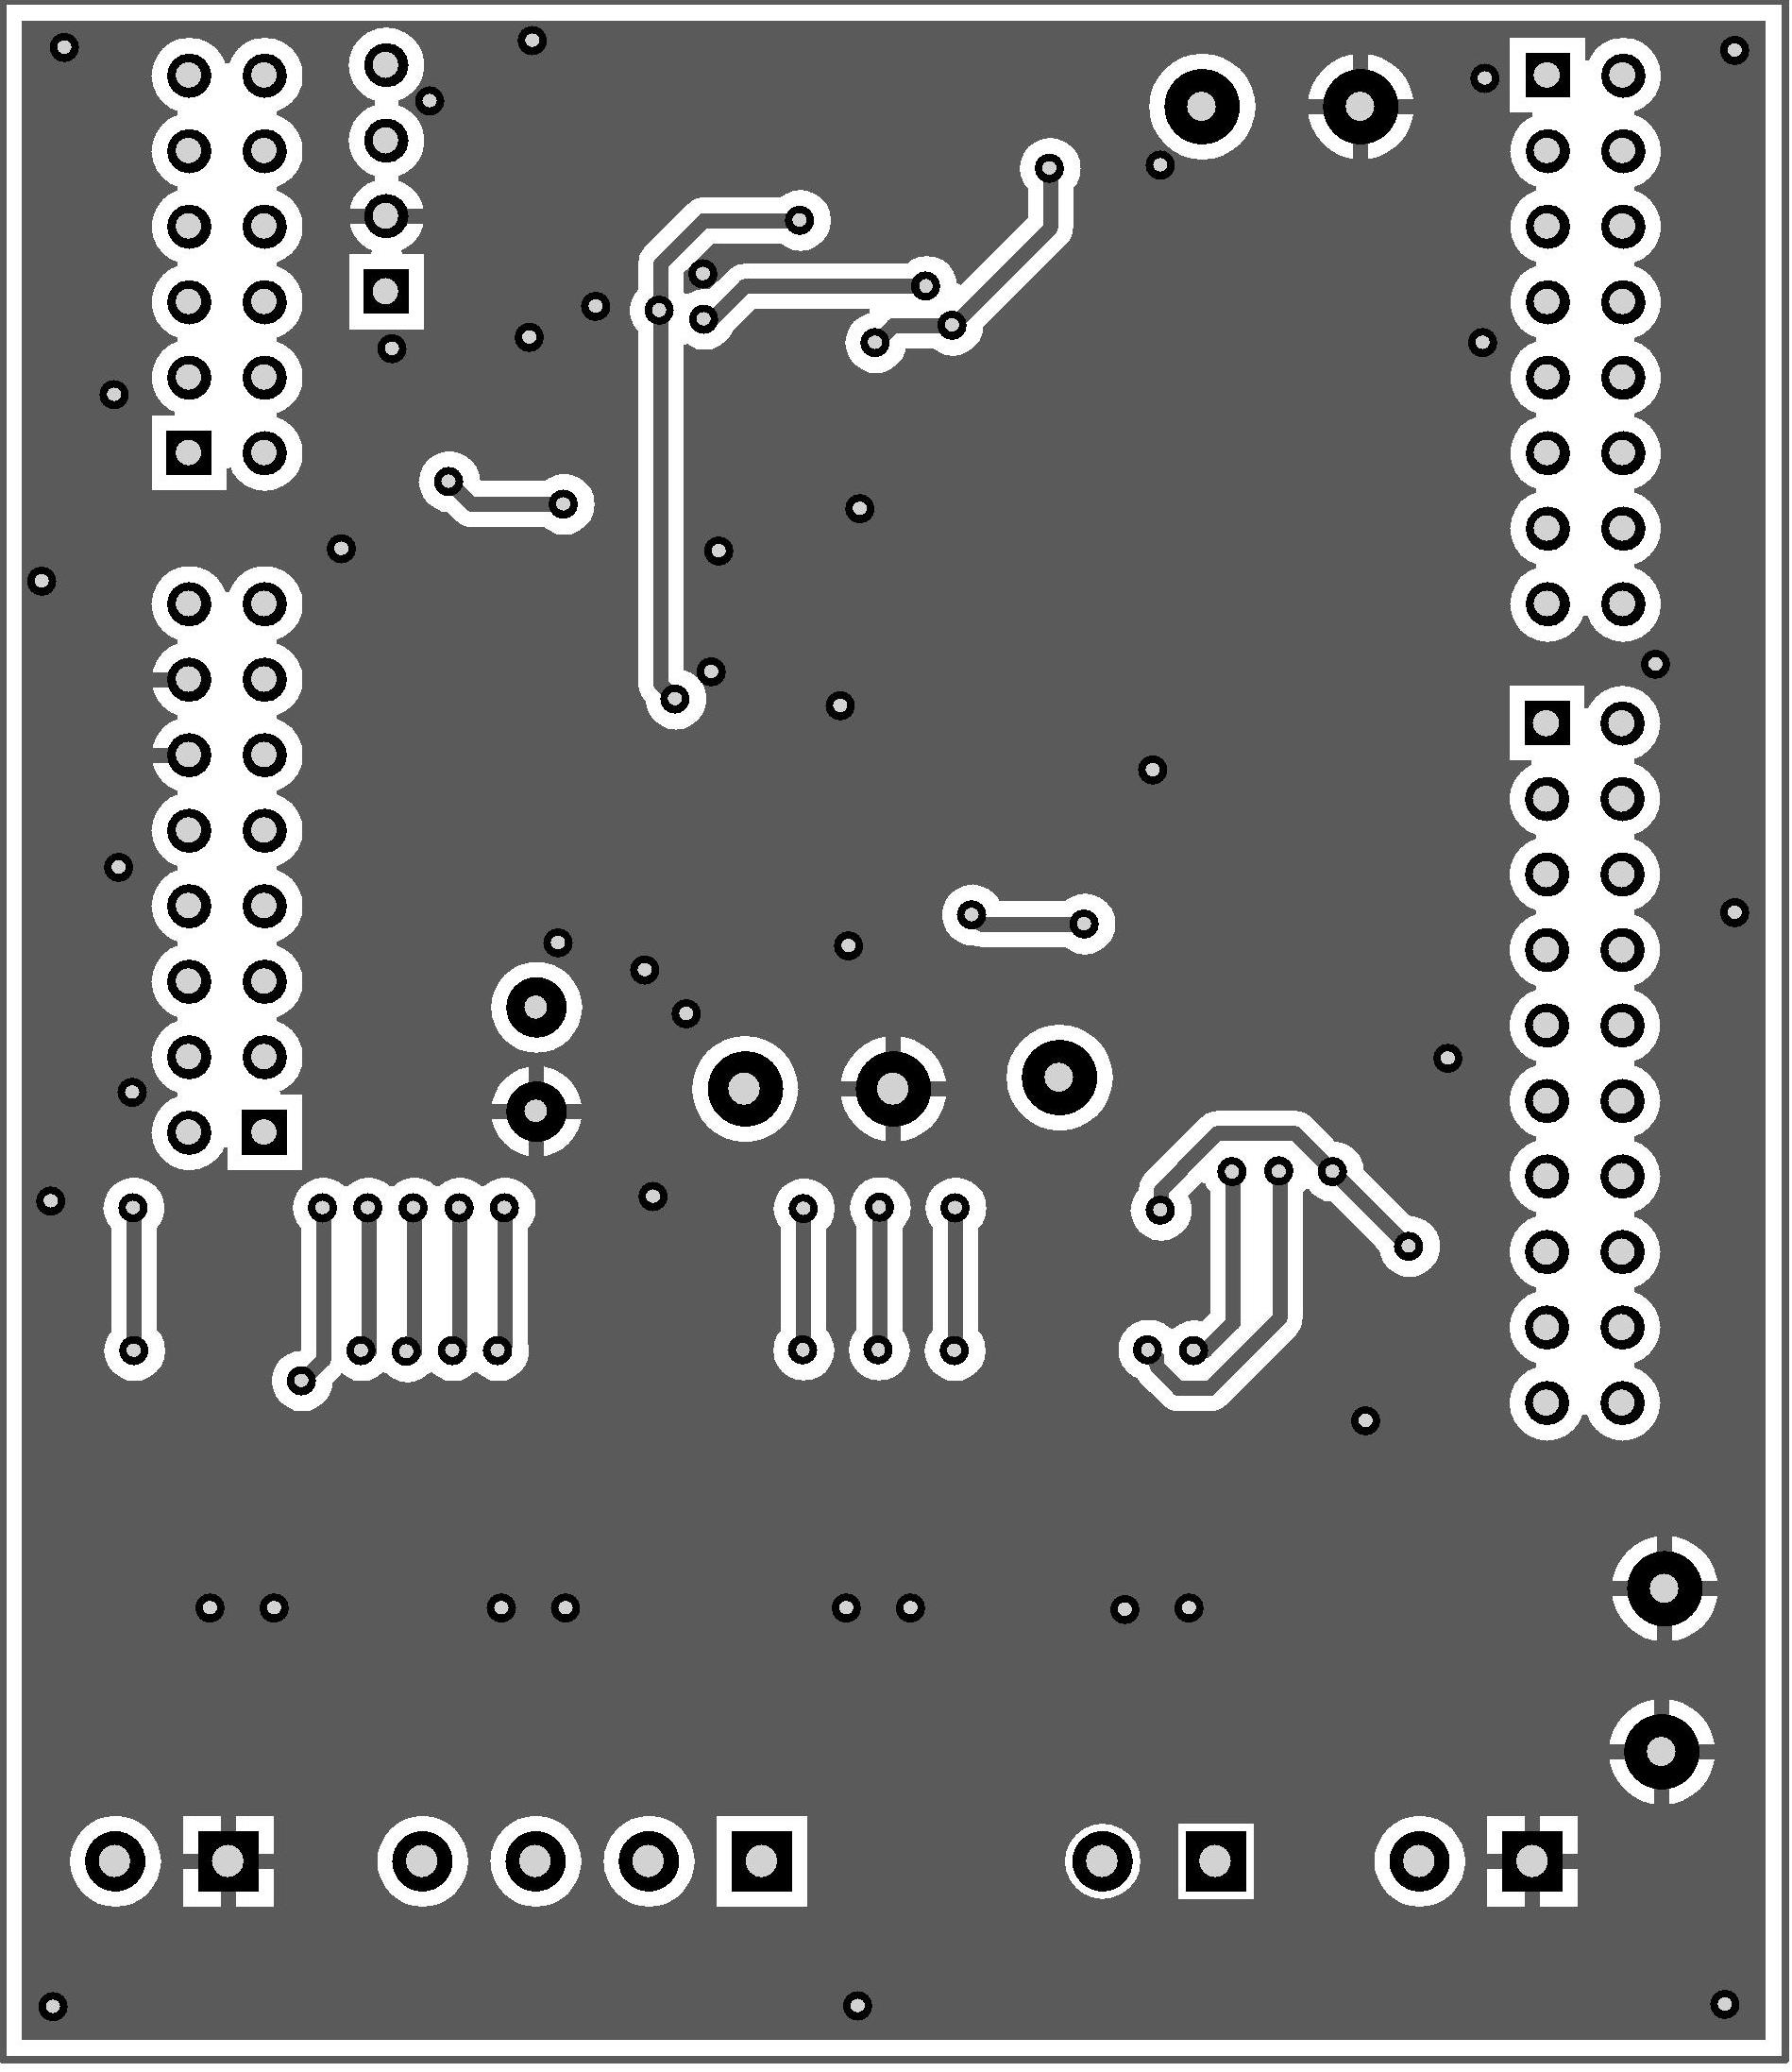
\includegraphics[width=6cm]{\EtPath/Bilder/DC_Stepper1.jpg}
            \caption{Bottom Layer}
            \label{fig:Bottom Layer}
        \end{minipage}
        \\[4ex]
        \begin{minipage}[hbt]{6cm}
            \centering
            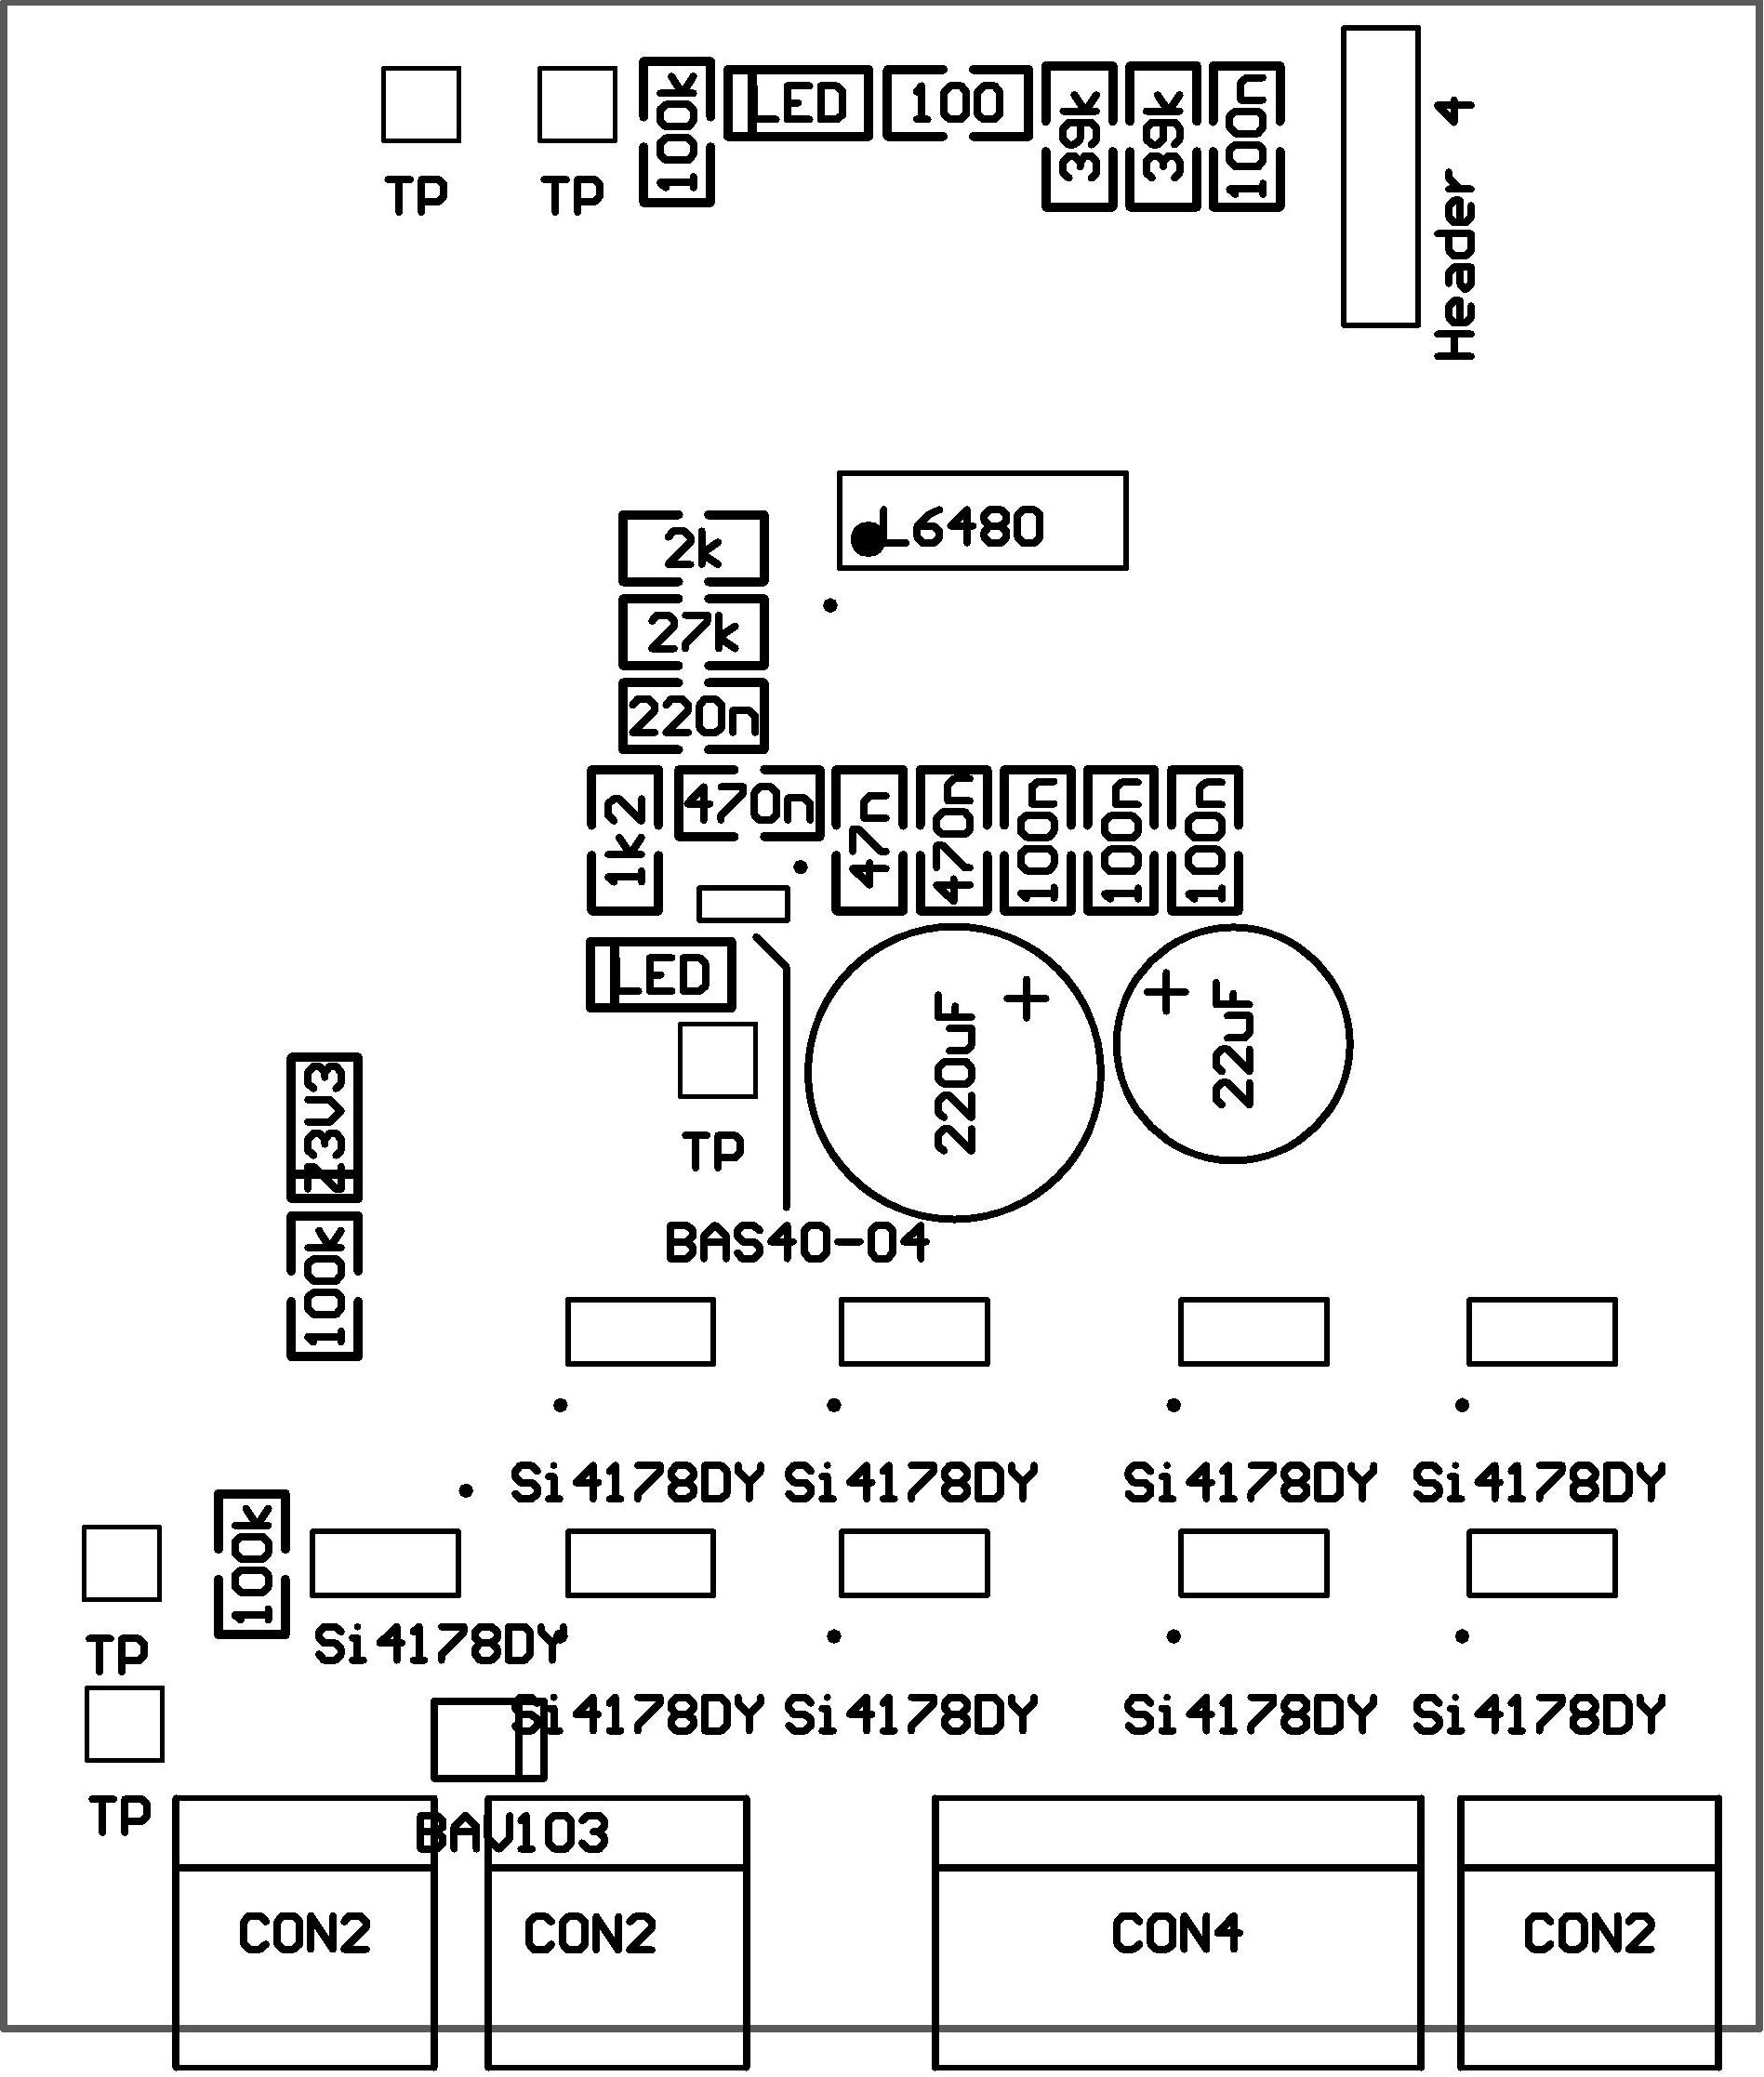
\includegraphics[width=6cm]{\EtPath/Bilder/DC_Stepper2.jpg}
            \caption{Werte}
            \label{fig:Werte}
        \end{minipage}
        \hspace{1.5cm}
        \begin{minipage}[hbt]{6cm}
            \centering
            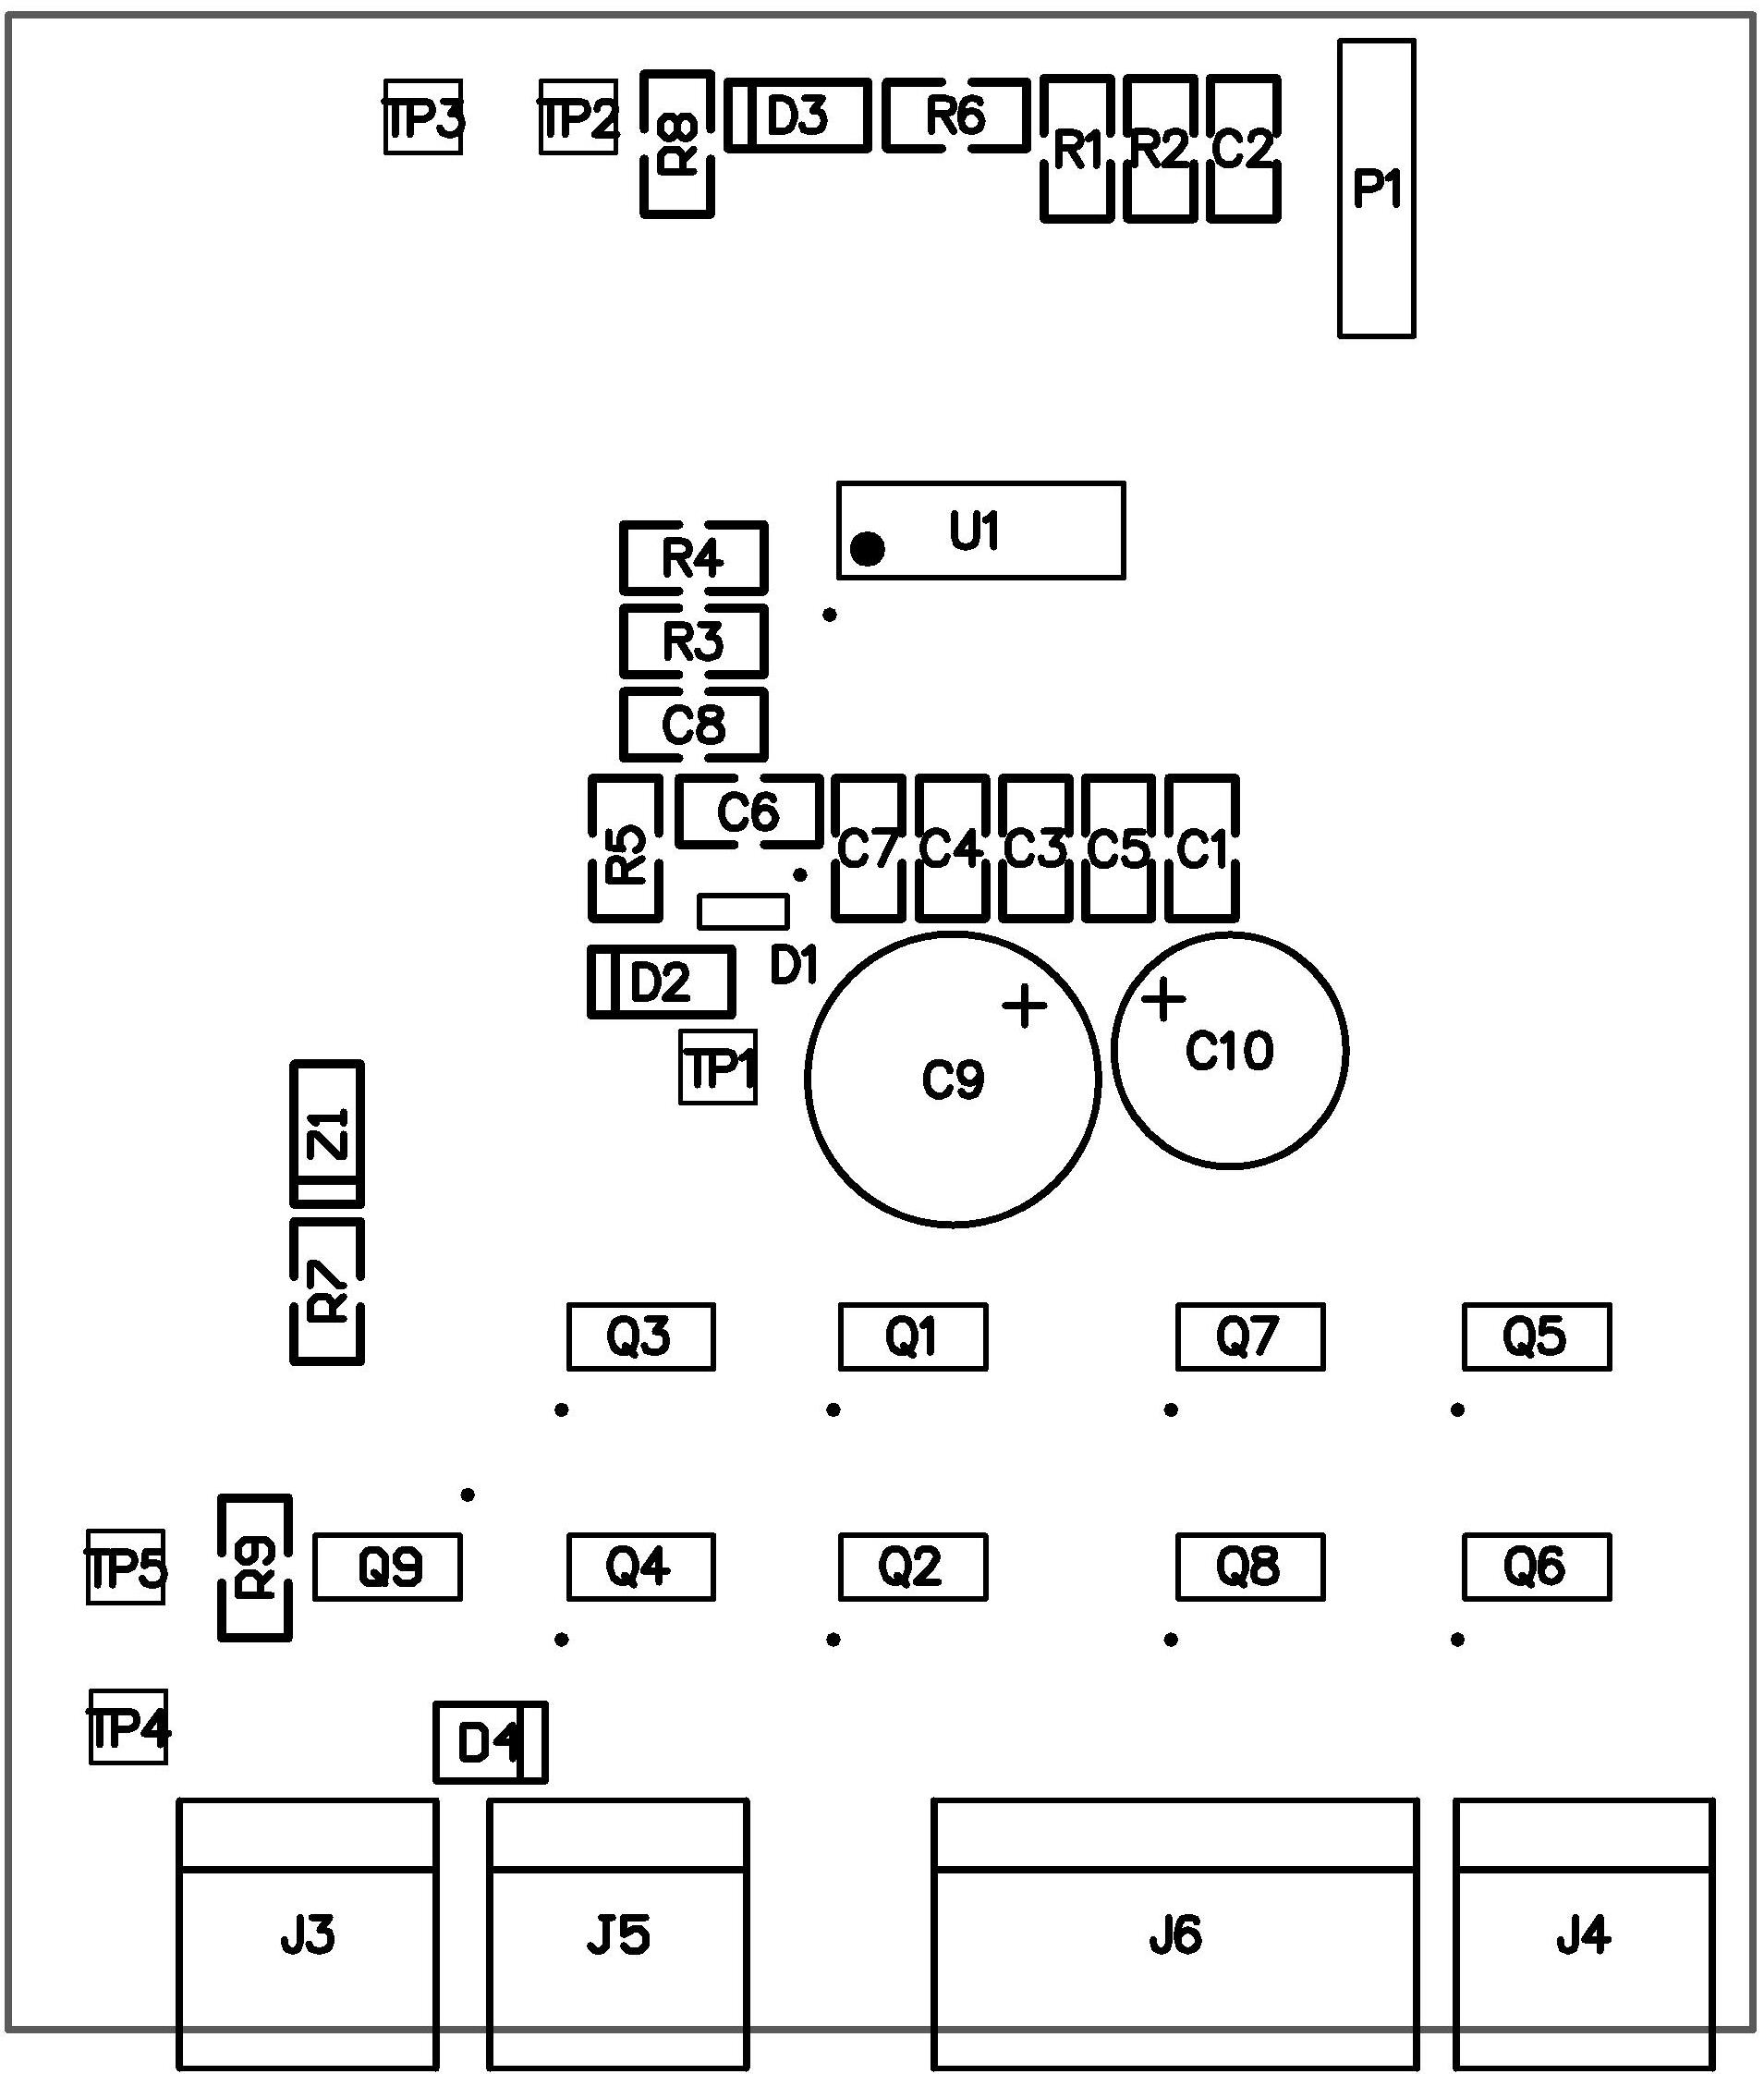
\includegraphics[width=6cm]{\EtPath/Bilder/DC_Stepper3.jpg}
            \caption{Bezeichnungen}
            \label{fig:Bezeichnungen}
        \end{minipage}
    \end{figure}
    % -----------------------------------------------------------------------------------
    \ifSTANDALONE
    \subsection{Print Design} \label{sec:PrintDesign}   
    \fi
    \ifEMBED
    \subsubsection{Print Design} \label{sec:PrintDesigna}
    \fi
    % TODO Betty, Korrektur durch Clirim        
    Der Adapterprint soll auf das Freedom-Board aufgesteckt werden und 
    möglichst klein sein. Der Print hat eine Grösse von 60mm x 70mm. Darauf 
    befinden sich die Anschlüsse für die Speisung, für den Motor, für weitere 
    Motoren und für einen End- oder Notschalter. Dazu werden stabile 
    Leiterplattenanschlüsse gewählt, welche auch die hohen Phasenströme des 
    Motors aushalten und zudem eine genug hohe Spannungsfestigkeit besitzen, 
    da die Motorenspannung bis 85V gewählt werden kann. Die eingesetzten 
    Leiterplattenanschlüsse sind für eine Spannung bis 300V und einem Strom 
    bis 8A geeignet. Dies ist ausreichend für diese Anwendung. Alle Bauteile 
    sind SMD, ausser den Leiterplattenanschlüssen und den Kondensatoren.
    \newpage
    Grundsätzlich werden folgende Regeln beim Design eingehalten: 
    \begin{itemize}
        \item Leiterbahnbreite 20mil
        \item Abstände zwischen Leiterbahnen und Polygonen 20mil
        \item keine rechten Winkel
        \item möglichst wenig Auskreuzungen auf dem Bottomlayer
        \item genügend grosse Pads 
        \item Verbindungen möglichst kurz halten
    \end{itemize}
    Da die Pins des L6480 näher als 20mil zueinander sind, können dort die 
    Regel für die Leiterbahnbreite und für den Abstand nicht eingehalten 
    werden. Deshalb werden für dieses Bauteil eigene Regeln definiert. Die 
    Leiterbahnen sind um den L6480 nur 8mil breit, werden jedoch sofort auf 
    20mil verdickt. Die Motorenphasen werden nicht mit Leiterbahnen an die 
    Anschlüsse geführt, sondern mit breiten Polygonen verbunden. Die 
    Auskreuzungen auf dem Bottomlayer werden vermieden, da einerseits 
    der erste Prototyp ohne Durchkontaktierung hergestellt wird, andererseits 
    da die GND-Fläche auf dem Bottomlayer möglichst nicht "verschnitten" 
    werden soll, um so EMV-Störungen abzuschirmen.
    Nach dem Layouten des ersten Prototypes folgt das Bestellen der Bauteile, 
    welche nicht im Elektroniklabor vorhanden sind. Die Stückliste ist in der 
    \autoref{Stückliste} zu finden. Der erste Prototyp wird von Hand 
    durchkontaktiert. Nach dem Bestücken mit der halbautomatischen 
    Bestückungsmaschine und dem Löten im Ofen wird der Prototyp in Betrieb 
    genommen. Die Inbetriebnahme zeigt, dass einige wenige Änderungen im 
    Layout nötig sind. Diese werden in einer überarbeiteten Version des 
    Adapterprints berücksichtigt. Der zweite Print wird maschinell 
    durchkontaktiert. Die Dokumente zur ersten Version sind im Anhang zu 
    finden. Die Bestückungsdokumente sind auf Seite \pageref{fig:Bottom Layer} 
    abgebildet.
    \begin{figure}[h]
        \centering
        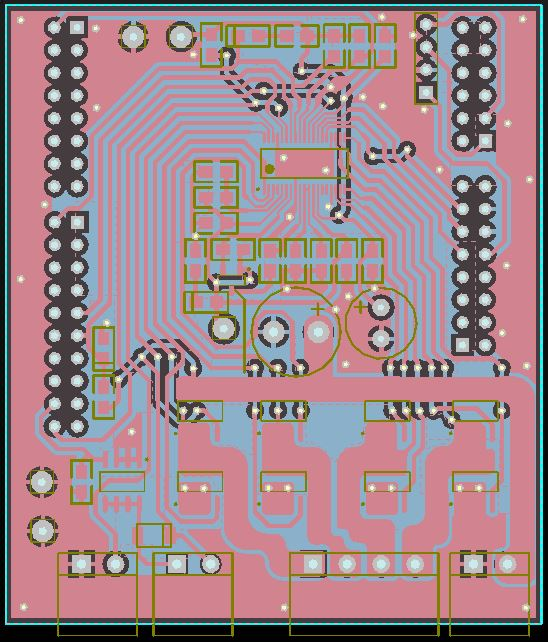
\includegraphics[width=5cm]{\EtPath/Bilder/printdesign.JPG}
        \caption{Printdesign mit Altium Designer}
        \label{fig:printdesign}
    \end{figure}
    \begin{table}
        \begin{zebralongtable}{p{2.5cm} p{3cm} p{2cm} p{4cm} p{1cm}} 
            \rowcolor{gray}
            \textbf{Bauteil}    & \textbf{Bezeichnung}  & \textbf{Lieferant} & \textbf{Bestellnummer}   &\textbf{Anz}\\
            Motor Contoller     & L6480H                & Mouser             & 511-L6480H               & 1\\   
            Shottkydiode        & BAS40-04-G            & Mouser             & 78-BAS40-04-E3-08        & 1\\ 
            Zenerdiode          & BZX585-B3V3           & Mouser             & 771-BZX585-B3V3          & 1\\ 
            Freilaufdiode       & BAV103                & Mouser             & 512-BAV103               & 1\\ 
            FET                 & Si4178DY              & PTA16              & 781-SI4178DY-TI-GE3      & 9\\ 
            LED                 & LSQ976                & Mouser             & 720-LSQ976-NR-1          & 2\\ 
        \end{zebralongtable}
        \caption{Stückliste (Bauteile nicht an Lager)} 
        \label{Stückliste}
    \end{table}  
    \newpage
    % -----------------------------------------------------------------------------------
    \ifSTANDALONE
    \subsection{Software}   \label{ch:Software} 
    \fi
    \ifEMBED
    \subsubsection{Software} \label{ch:Software}
    \fi
    Für die einfache Einbindung des Schrittmotortreibers in die Software der 
    jeweiligen Teams wird eine Bibliothek erstellt. Diese besteht aus den 
    Dateien \verb?l6480.c? und \verb?l6480.h?, welche in eigene Software 
    eingebunden werden kann. 
    \begin{lstlisting}[caption={Einbinden der Bibliothek}]
#include l6480.h
    \end{lstlisting}
    Diese Bibliothek bietet Funktionen um alle Register des 
    Schrittmotortreibers zu beschreiben und zu lesen. Ausserdem ist jeder 
    Befehl des Treibers implementiert. Die Bibliothek ist mit Doxygen 
    dokumentiert. In der entsprechenden Dokumentation ist die Schnittstelle 
    der Bibliothek beschrieben. 
    Damit die Bibliothek mit dem Schrittmotortreiber kommunizieren kann, muss 
    eine SPI Schnittstelle zur breeitgestellt werden. Dazu sind die Funktionen 
    \verb?spi_write(uint8_t *data)? und \verb?spi_read(uint8_t *data)? so zu 
    ergänzen, dass sie jeweils ein Byte über SPI senden respektive empfangen.  
    Über die Konstante \verb?PL_FRDM? ist die SPI Schnittstelle auf einem 
    FRDM-KL25Z von Freescale einschaltbar. Die SPI Komponente heisst dabei 
    Stepperspi. Alle notwendigen Komponenten sind in \autoref{tab:comp_frdm} 
    aufgeführt. 
    \begin{lstlisting}[caption={Definition der Plattform für das FRDM-KL25Z}]
#define PL_FRDM
    \end{lstlisting}
    \begin{table}[h!]
        \centering
        \begin{zebratabular}{p{0.11\textwidth}p{0.14\textwidth}p{0.5\textwidth}}
            \rowcolor{gray}
            Name        & Komponente    & Beschreibung \\
            Stepperspi  & SynchroMaster & SPI \\
            WAIT1       & Wait          & Delays \\
            STP\_BSY    & ExtInt        & Interrupt für das Signal Busy \\
        \end{zebratabular}
        \caption{Komponenten bei Verwendung auf einem FRDM-KL25Z}
        \label{tab:comp_frdm}
    \end{table}
    Zudem kann mit der Konstante \verb?PL_HAS_SHELL?  die Unterstützung einer 
    Shell-Komponente aktiviert werden. Die für die Shell zusätzlich 
    notwendigen Komponenten sind in \autoref{tab:comp_shell} aufgeführt. 
    \begin{lstlisting}[caption={Definition für Shell-Unterstützung}]
#define PL_HAS_SHELL
    \end{lstlisting}
    \begin{table}[h!]
        \centering
        \begin{zebratabular}{p{0.11\textwidth}p{0.14\textwidth}p{0.5\textwidth}}
            \rowcolor{gray}
            Name        & Komponente    & Beschreibung \\
            CLS1        & Shell         & Shell \\
            UTIL1       & Utility       & Funktionen für die Verarbeitung von Strings \\
            Shell       & -             & Funktionen für das Senden von Strings über die Schell \\
        \end{zebratabular}
        \caption{Komponenten bei Verwendung der Shell}
        \label{tab:comp_shell}
    \end{table}

    \clearpage
    \ifSTANDALONE
    \subsubsection{Test auf Computer}   \label{sec:Software_test} 
    \fi
    \ifEMBED
    \paragraph{Test} auf Computer \label{sec:Software_test}
    \fi
    Wird die Konstante \verb?PL_FRDM?  nicht gesetzt, kann die Bibliothek auf 
    einem Computer kompiliert und getestet werden. Das ermöglicht das Testen 
    der Bibliothek ohne Hardware. Die Daten werden dabei nicht über SPI 
    geschickt, sondern auf die Standardausgabe ausgegeben. 
    \begin{lstlisting}[caption={Beispielprogramm für den Test der Bibliothek auf dem Computer}, label={lis:test_source}]
#include "stdio.h"
#include "drv/l6480.h"

int main(void) {
    l6480_init();
    printf("hardhiz\n");
    l6480_cmd_hardhiz();
    printf("run 1 2\n");
    l6480_cmd_run(1, 2);
    return 0;
}
    \end{lstlisting}
    \begin{lstlisting}[caption={Ausgabe vom Testprogramm in \autoref{lis:test_source}}]
hardhiz
write: 0xA8
run 1 2
write: 0x51
write: 0x0
write: 0x0
write: 0x2
    \end{lstlisting}






%    Die Software auf dem Freedom-Board dient als Schnittstellensoftware. Sie 
%    nimmt die Befehle der zentralen Recheneinheit über USB/UART an und sendet 
%    diese an den Motor Controller l6480 sowie das Pneumatikventil weiter. Die 
%    Software wurde mit der Entwicklungsumgebung Kinetis Design Studio von 
%    Freescale entwickelt. Diese Umgebung bietet ein Tool, welches Processor 
%    Expert heisst. Dieses erlaubt es, Komponenten wie z.B. einen 
%    Analog-Digital-Wandler in das Projekt zu integrieren. Die Konfiguration 
%    solcher Komponenten kann mit dem Component Inspector vorgenommen werden, 
%    ohne dass einzelne Register des Mikrocontrollers beschrieben werden 
%    müssen. Die Komponenten stammen von der Internetseite 
%    http://steinerberg.com/EmbeddedComponents/ und können dort gratis 
%    gedownloadet werden.
%    \\\\
%    Die Software auf dem Freedom-Board beinhaltet folgende fünf Komponenten 
%    mit ihren Aufgaben: 
%    \begin{itemize}
%        \item FreeRTOS:         Ein Open-Source-Echtbetriebszeitsystem für 
%            Mikroprozessoren und Mikrocontroller.  
%        \item Shell:            Die Schnittstelle zur zentralen Recheneinheit. 
%            Sie vergleicht die von der zentralen Recheneinheit ankommenden 
%            Befehle und ruft die entsprechenden Funktionen auf. 
%        \item SynchroMaster:    SPI-Komponente für die Kommunikation mit dem 
%            Schrittmorotren-IC L6480. 
%        \item LED:              Anzeige auf dem Freedom-Boarad.
%        \item Bit:              Ansteuerung des Pneumatikventils.
%    \end{itemize}
%    \textbf{Schrittmotorentreiber}\\
%    Im Datenblatt des L4680 sind die verschiedenen Bitfolgen, welche einzelnen 
%    Kommandos entsprechen, dokumentiert. In der \autoref{fig:command} ist ein 
%    Beispieles eines solchen Kommandos aus dem Datenblatt des l6480 zu sehen, 
%    welches den Befehl RUN beschreibt. In diesem Beispiel werden 4 Bytes 
%    einzeln über die SPI-Schnittstelle gesendet: 
%    \begin{enumerate}
%        \item Bitfolge für das Kommando RUN, sowie die Richtung (DIR) der Bewegung
%        \item Bit 16 bis 19 der Geschwindigkeit, mit welcher sich der Motor dreht
%        \item Bit 8 bis 15 der Geschwindigkeit
%        \item Bit 0 bis 7 der Geschwindigkeit
%    \end{enumerate}
%    \begin{figure}[h!]
%        \centering
%        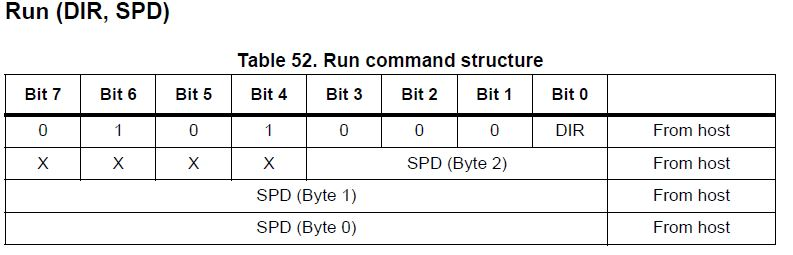
\includegraphics[width=10cm]{\EtPath/Bilder/command_example.JPG}
%        \caption{Beispiel eines Kommandos aus dem Datenblatt des l6480}
%        \label{fig:command}
%    \end{figure}
%    Der Treiber beinhaltet die Funktionen, welche die richtigen Bitfolgen über 
%    SPI an den L6480 senden. Fast alle dieser Funktionen wurden in 
%    Zusammenarbeit mit dem PREN-ET Team von Daniel Winz implementiert.  
%    \\\\
%    \textbf{Shell}\\
%    Für das Pneumatikventil und den Steppertreiber wurden Shellfunktionen 
%    implementiert. Erhält die Shell ein Kommando von der zentralen 
%    Recheneinheit, so wird die Eingabe ausgewertet und die entsprechende 
%    Shellfunktion ausgeführt. Die von der zentralen Recheneinheit geparsten 
%    Befehle sind:  
%    \begin{itemize}
%        \item l6480 run [f/r] [speed]
%        \item l6480 reset
%        \item l6480 softstop
%        \item l6480 hardstop
%        \item l6480 softhiz
%    \end{itemize}
%    für die Steuerung des Motor Controllers, sowie
%    \begin{itemize}
%        \item vent shoot
%    \end{itemize}
%    für die Steuerung des Pneumatikventils. 
%    \\\\
%    Der Befehl "l6480 run" lässt den Motor in Vorwärtsrichtung [f] oder 
%    Rückwärtsrichtung [r] mit der in [speed] definierten Geschwindigkeit 
%    drehen. "l6480 reset" konfiguriert den l6480 und bestromt den Motor, so 
%    dass dieser ein Haltemoment aufweist. Um den Motor ohne Haltemoment 
%    bewegen zu können, wird der Befehl "l6480 softhiz" verwendet, welcher die 
%    H-Brücke ausschaltet. 
    

    \ifSTANDALONE
\section{Ausblick}
\fi
\ifEMBED
\subsection{Ausblick}
\fi
	In einem nächsten Schritt soll der L6480 bestellt und in einer 
    Testschaltung getestet werden. Weiter soll ein Schema und ein Layout 
    geplant und produziert werden, welche alle Teammitglieder in ihrem Projekt 
    verwenden können, falls sie dies benötigen. 

    \clearpage
\fi
    
\ifREVIEW
    \section{Fazit}
    Die teamübergreifende Zusammenarbeit in PREN-ET hat sich extrem bewährt. 
    Auf diese Weise konnten komplexere und anspruchsvollere Lösungen 
    realisiert werden. Dementsprechend war der Lerneffekt massiv grösser. Die 
    ET-Zusammenarbeit hat sich nicht nur in der Erhöhung der 
    \enquote{man-power} niedergeschlagen, sondern auch in der Vielfalt der 
    Themen und deren spezifischen Problemen respektive Lösungen. So konnte zum 
    Beispiel die Ansteuerung eines Bürstenlosen Motors von Grund auf 
    erarbeitet und realisiert werden. Für die Ansteuerung des Schrittmotors 
    wurde ein Integrierter Treiber mit aufwendigem Interface verwendet, 
    welches dank der Zusammenarbeit komplett implementiert werden konnte. Beim 
    Review von Schemas, finden von Fehlern im Code und beim Erstellen und 
    Korrigieren der Dokumentation war es ein grosser Vorteil, dass mehrere 
    Elektrotechnik-Studierende zusammenarbeiten konnten. 
    
    \noindent
    Zu begin war es zeitintensiv, die Gruppen, die Tools und das gemeinsame 
    Vorgehen zu definieren und umzusetzen. Sobald dies erledigt war, 
    funktionierte die Zusammenarbeit innerhalb von PREN-ET ausserordentlich 
    gut. Als ein weiterer kritischer Punkt bei teamübergreifenden Arbeiten 
    stellte sich die Dokumentation heraus. So muss eine Dokumentation 
    erarbeitet werden, welche bei jedem Team in die Teamdokumentation 
    eingegliedert werden muss. Zudem muss besonders darauf geachtet werden, 
    dass fremde Texte korrekt als solche gekennzeichnet sind. 

\fi
\setlength\bibitemsep{1.5\itemsep}
%Folgende Zeile auskommentieren, damit nur gebrauchte Literatur erscheint
%\nocite{*}
\renewcommand{\refname}{Literatur- und Quellenverzeichnis}
% \bibliographystyle{apacite} set in layout.sty -> do not try to set it here again!
\bibliography{\BIBLIOGRAPHY}

\listoffigures
\listoftables

\ifBLDC 
    \appendix      
    \begin{appendix}
        \clearpage
        \pagenumbering{Roman}
        \renewcommand{\EtPath}{src/bldc}
        \begin{landscape}
    \ifSTANDALONE
    \section{Schema des BLDC-Boards}
    \fi
    \ifEMBED
    \subsection{Schema des BLDC-Boards}
    \fi
    \label{apx:Schema_BLDC} 
    \ifSTANDALONE
    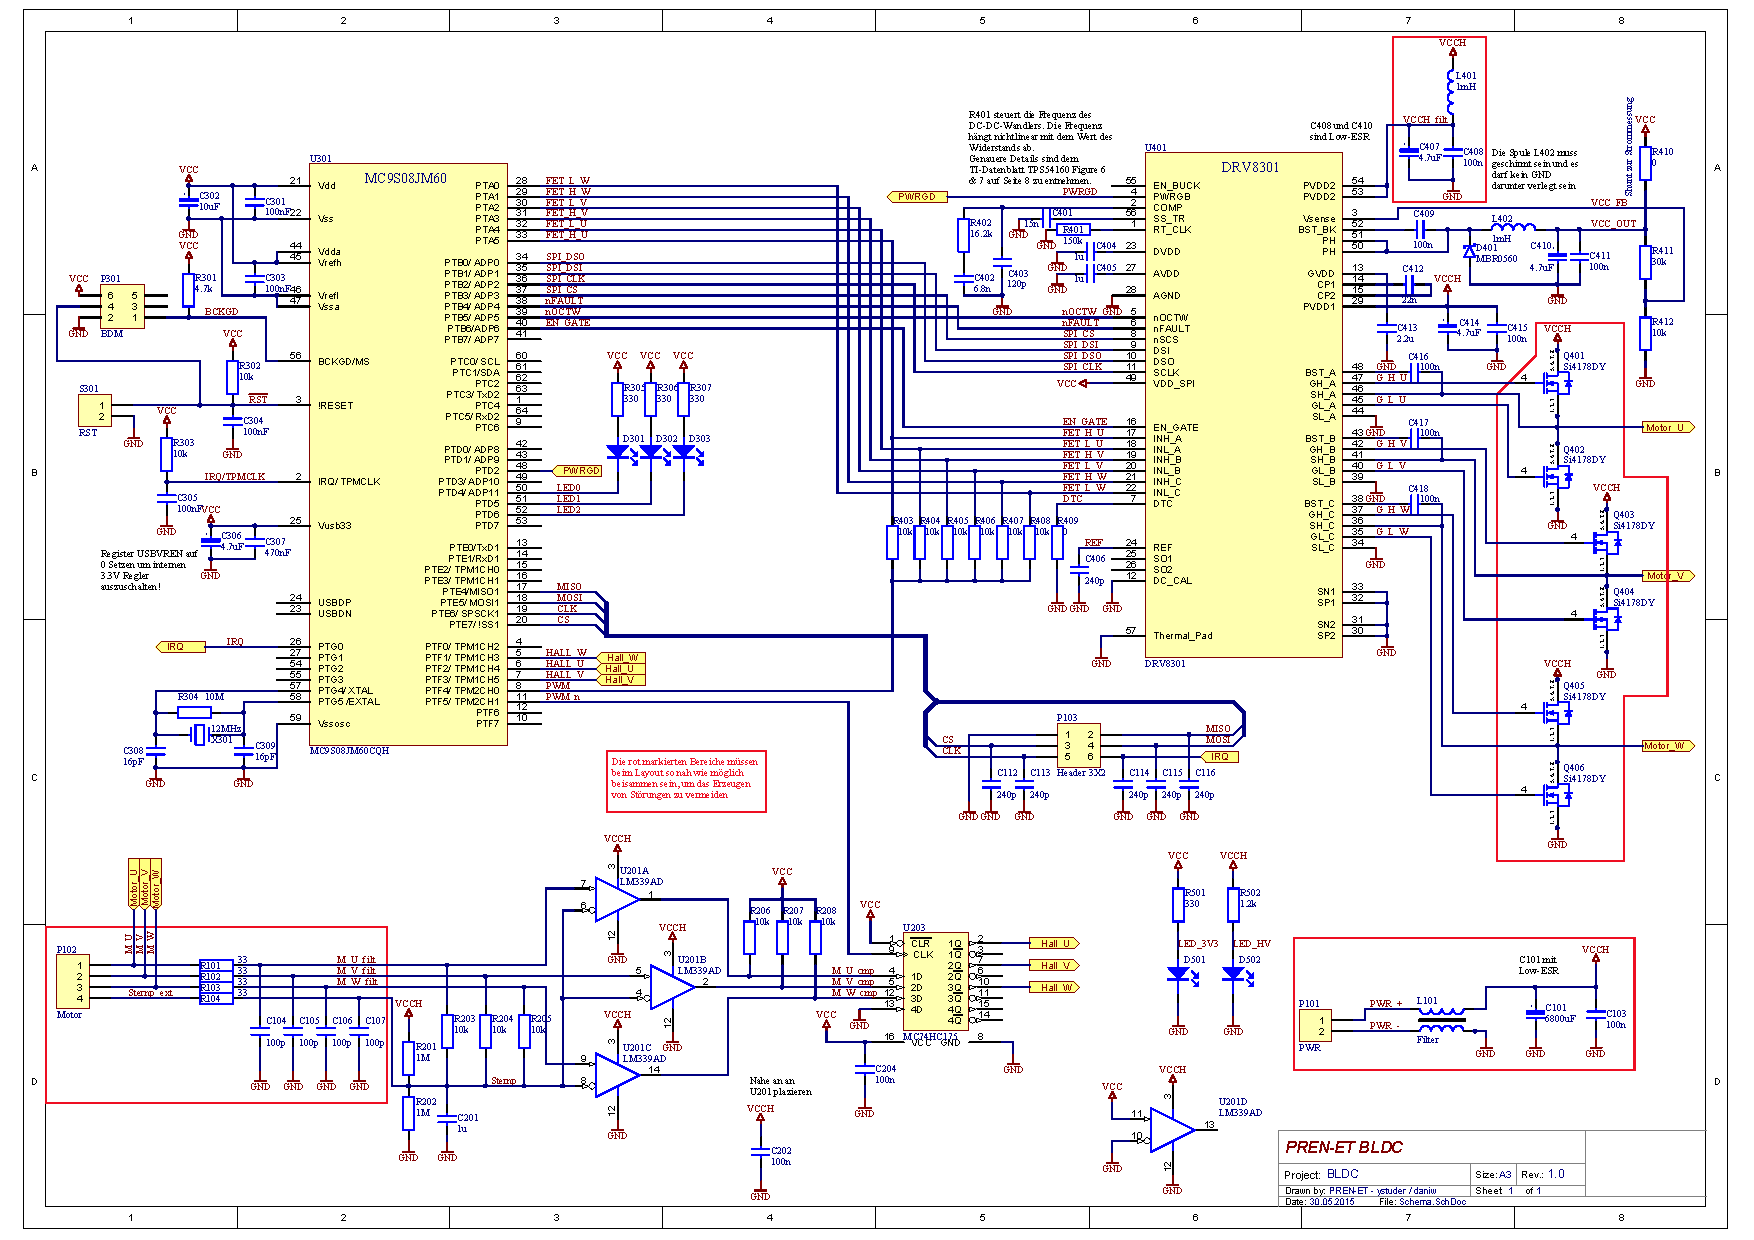
\includegraphics[page=1,scale=0.78,clip,trim=4mm 1.5mm 4mm 1mm]
        {\EtPath/Bilder/SchemaBLDC.pdf}
    \fi
    \ifEMBED
    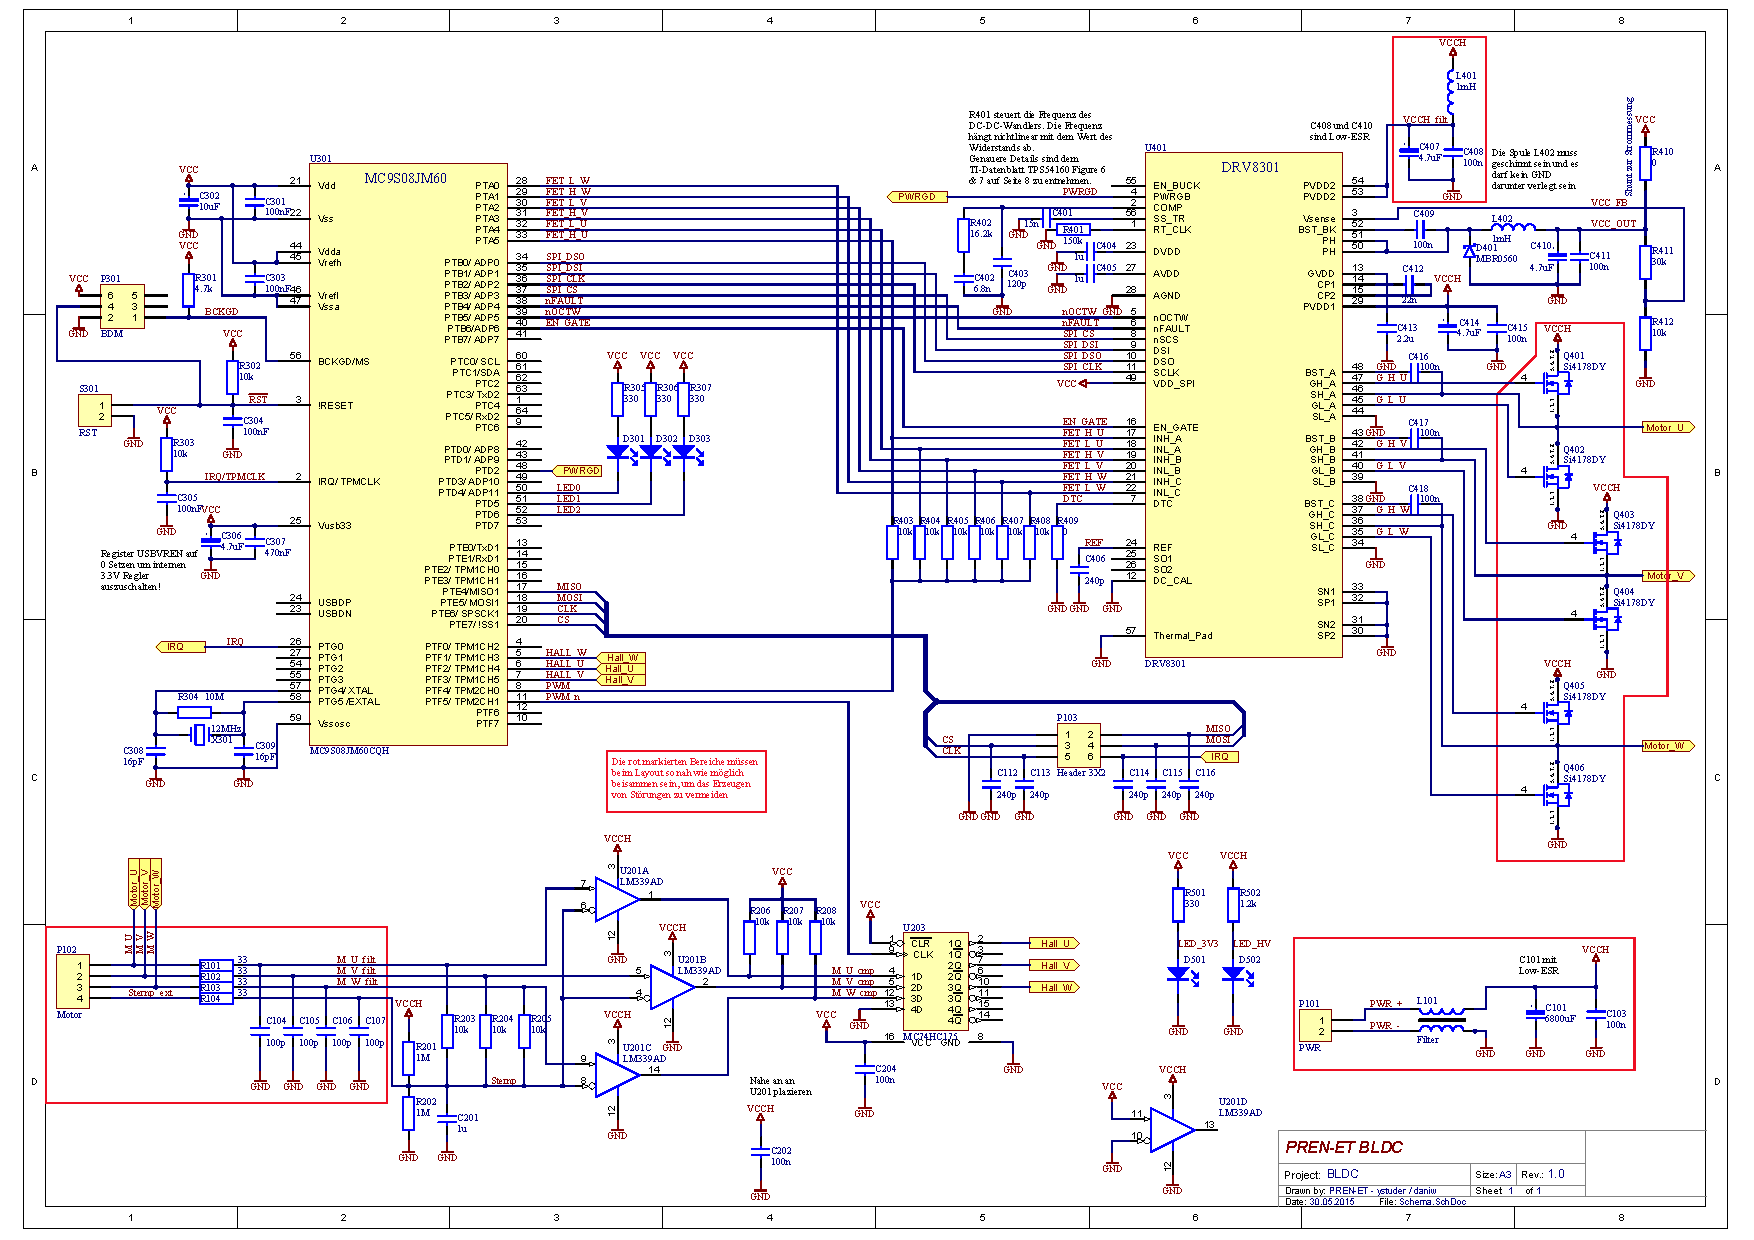
\includegraphics[page=1,scale=0.74,clip,trim=4mm 1.5mm 4mm 1mm]
        {\EtPath/Bilder/SchemaBLDC.pdf}
    \fi   
\end{landscape}

    \end{appendix}
\fi
